\documentclass[fontsize=11pt,twoside=true,headsepline,footsepline,headinclude,footinclude=false,a4paper,listof=totoc,bibliography=totoc,openright]{scrbook}
\usepackage[T1]{fontenc}
\usepackage[utf8]{inputenc}
\usepackage{xspace}
\usepackage{graphicx}
\usepackage[lighttt]{lmodern}
\usepackage[svgnames]{xcolor}
\usepackage{charter}
\usepackage[final]{microtype}
\usepackage{tgheros}
\usepackage[english,ngerman]{babel}
%\usepackage{scrpage2}
\usepackage[top=3.75cm,left=2.75cm,right=2.75cm,bottom=3.75cm,bindingoffset=0.5cm,heightrounded,marginparwidth=2cm,marginparsep=0.25cm,headsep=2em,footskip=3em]{geometry}
%\usepackage{titlesec}
\setkomafont{disposition}{\normalfont\bfseries} % use serif font for headings
\linespread{1.05} % adjust line spread for mathpazo font
\usepackage[sc]{mathpazo}
\usepackage[style=numeric,sorting=ynt]{biblatex}
\usepackage[autostyle]{csquotes}
\usepackage{enumitem}
\usepackage{listings}
\usepackage{rotating}
\usepackage{hyperref}
\usepackage{float}


\usepackage{csquotes}
\usepackage{textcomp}
\usepackage{comment}
\usepackage{listings}
\usepackage{graphicx}
\usepackage{caption}
\usepackage{subcaption}
\usepackage{amsmath}
\usepackage{gensymb}

\definecolor{codegreen}{rgb}{0,0.6,0}
\definecolor{codegray}{rgb}{0.5,0.5,0.5}
\definecolor{codepurple}{rgb}{0.58,0,0.82}
\definecolor{backcolor}{rgb}{0.95,0.95,0.92}

\setcounter{biburllcpenalty}{7000}
\setcounter{biburlucpenalty}{8000}

%%%%%%%%%%%%%%%%%%%%%
% xspace und deutsche Anführungszeichen
%%%%%%%%%%%%%%%%%%%%%
\xspaceaddexceptions{\grqq}

%%%%%%%%%%%%%%%%%%%%%%%%%%
% Überschriften formatieren
%%%%%%%%%%%%%%%%%%%%%%%%%%
\iffalse
\titleformat{\chapter}[display]
      {\sffamily\bfseries\Large}
      {\filright\MakeUppercase{\chaptertitlename} \Huge\thechapter}
      {1ex}
      {\titlerule\vspace{1ex}\filleft}
      [\vspace{1ex}\titlerule]
\titleformat*{\section}{\sffamily\bfseries\Large}
\fi

%%%%%%%%%%%%%%%%%%%%%%%%%%
% Kommandos und Umgebungen
%%%%%%%%%%%%%%%%%%%%%%%%%%
\newenvironment{abstract}%
{\thispagestyle{empty}\cleardoublepage 
 \null \begin{center}%
 \textbf{\sffamily \Large \abstractname} \end{center}\vspace*{3cm}}%
{\vfill \null }

\newcommand{\thetitle}{Titel fehlt}
\newcommand{\Titel}[1]{\renewcommand{\thetitle}{#1\xspace}}

\newcommand{\matrikelnummer}{Matrikelnummer fehlt}
\newcommand{\Matrikelnummer}[1]{\renewcommand{\matrikelnummer}{#1\xspace}}

\newcommand{\authorname}{Autor fehlt}
\newcommand{\Autor}[1]{\renewcommand{\authorname}{#1\xspace}}

\newcommand{\studiengang}{Studiengang fehlt}
\newcommand{\Studiengang}[1]{\renewcommand{\studiengang}{#1\xspace}}

\newcommand{\thesistype}{Typ der Arbeit fehlt}
\newcommand{\Arbeitstyp}[1]{\renewcommand{\thesistype}{#1\xspace}}

\newcommand{\gutachtereins}{Erstgutachter fehlt}
\newcommand{\Erstgutachter}[1]{\renewcommand{\gutachtereins}{#1\xspace}}

\newcommand{\gutachterzwei}{Zweitgutachter fehlt}
\newcommand{\Zweitgutachter}[1]{\renewcommand{\gutachterzwei}{#1\xspace}}

\newcommand{\abgabedatum}{Abgabedatum fehlt}
\newcommand{\Abgabe}[1]{\renewcommand{\abgabedatum}{#1\xspace}}

\newcommand{\betreuer}{Betreuer fehlt}
\newcommand{\Betreuer}[1]{\renewcommand{\betreuer}{#1\xspace}}


\lstdefinestyle{mystyle}{
    backgroundcolor=\color{backcolor},   
    commentstyle=\color{codegreen},
    keywordstyle=\color{magenta},
    numberstyle=\tiny\color{codegray},
    stringstyle=\color{codepurple},
    basicstyle=\footnotesize,
    breakatwhitespace=false,         
    breaklines=true,                 
    captionpos=b,                    
    keepspaces=true,                 
    numbers=left,                    
    numbersep=5pt,                  
    showspaces=false,                
    showstringspaces=false,
    showtabs=false,                  
    tabsize=2
}
\lstset{emph={%  
    as, True, False%
    },emphstyle={\color{magenta}}%
}%
 
\lstset{style=mystyle}

\Arbeitstyp{Masterarbeit}
\Studiengang{Informatik}
\Autor{Sebastian Rossi}
\Matrikelnummer{1475010}
\Titel{Individualisierbarer Konstruktionsplaner mit automatischer Bauplandeduktion}
\Erstgutachter{Prof.\ Dr.\ Wolfgang Reif}
\Zweitgutachter{Prof.\ Dr.\ Bernhard Bauer}

\Abgabe{8. Januar 2023}
\Betreuer{Constantin Wanninger}

\bibliography{bib/bibliography}

\begin{document}
\selectlanguage{ngerman}
%%%%%%%%%%%%%%%%%%%%%%%%%%%%%%%%%%%%%%%%%%%%%%%%%%%%%%%%%%%%%%%%%%%%%%%%%%%%%%%%%%%%
%%% Title-Page
\begin{titlepage}
\thispagestyle{empty}
\begin{center}
    
\includegraphics[height=3.2cm]{fig/unilogo/Uni-Logo.pdf}
\end{center}

\vspace{8mm}
\begin{center}
{\Large
{\bfseries \bfseries Institut für Software \& Systems Engineering}\\
Universitätsstraße 6a \hspace{0.25cm} D-86159 Augsburg\\[5mm]

\includegraphics[height=1.5cm]{fig/unilogo/ISSE-Logo.pdf}
}
\end{center}

\vspace{1cm}
\begin{center}
{\large \textbf{\thesistype im Studiengang}\\[0.5ex]
\textbf{\glqq \studiengang\grqq}}
\end{center}
\vspace{1cm}

% Titel
\begin{center}
{\Huge \bfseries \thetitle}
\end{center}

\vspace{1.5cm}
% Autor
\begin{center}
{\LARGE \authorname}
\end{center}
\end{titlepage}




%%%%%%%%%%%%%%%%%%%%%%%%%%%%%%%%%%%%%%%%%%%%%%%%%%%%%%%%%%%%%%%%%%%%%%%%%%%%%%%%%%%%
%%% Advisor-Page
%%%%%%%%%%%%%%%%%%%%%%%%%%%%%%%%%%%%%%%%%%%%%%%%%%%%%%%%%%%%%%%%%%%%%%%%%%%%%%%%%%%%
\newpage
\thispagestyle{empty}
\mbox{}
\newpage
\thispagestyle{empty}
\begin{center}
    
\includegraphics[height=3.2cm]{fig/unilogo/Uni-Logo.pdf}
\end{center}

\vspace{4mm}
\begin{center}
{\Large
{\bfseries \bfseries Institut für Software \& Systems Engineering}\\
Universitätsstraße 6a \hspace{0.25cm} D-86135 Augsburg\\[5mm]

\includegraphics[height=1.5cm]{fig/unilogo/ISSE-Logo-Farbig.pdf}
}
\end{center}

\vspace{1cm}
% Titel
\begin{center}
{\LARGE \bfseries \thetitle}
\end{center}

\vspace{8mm}

% Autor
\begin{center}
{\large \authorname}
\end{center}
\vfill
% Daten zur Arbeit
\begin{center}
\begin{table}[h]
\centering
\begin{tabular}{ll}
Erstgutachter: & \gutachtereins \\
Zweitgutachter: & \gutachterzwei \\
Matrikelnummer: & \matrikelnummer \\
Abgabe der Arbeit: & \abgabedatum \\
Betreuer: & \betreuer \\
\end{tabular}
\end{table}
\end{center}

%%%%%%%%%%%%%%%%%%%%%%%%%%%%%%%%%%%%%%%%%%%%%%%%%%%%%%%%%%%%%%%%%%%%%%%%%%%%%%%%%%%%
%%% Statement-Page
\newpage
\thispagestyle{empty}
\mbox{}
\newpage
\thispagestyle{empty}

\centerline{\textbf{\sffamily\Large Erklärung}}

\vspace{3cm}
\noindent
Hiermit versichere ich, dass ich diese \thesistype selbständig verfasst habe.
Ich habe dazu keine anderen als die angegebenen Quellen und Hilfsmittel
verwendet.

\vspace{2.5cm}
\begin{flushleft}
%select german for formatting the date
\selectlanguage{ngerman}
Augsburg, den \abgabedatum \hfill \authorname
\end{flushleft}

\newpage
\thispagestyle{empty}
\mbox{}


\cleardoublepage

\pagenumbering{roman}

%\input{txt/thanks}

\begin{abstract}
    Aufgrund des sich zuspitzenden Fachkräftemangels in der Baubranche ist es nicht verwunderlich, dass zunehmend Bestrebungen in Richtung der Automatisierung dieses Industriebereichs angestellt werden.
Möglich sind automatisierte Bauprojekte erst aufgrund der fortschreitenden Digitalisierung und Vereinheitlichung durch internationale Standards.
Denn der Automatisierung liegt oftmals ein nicht zu unterschätzender, vorangehender Planungsaufwand zugrunde, welcher erst dadurch softwareseitig durchführbar wird.
Diese Arbeit beschäftigt sich mit den Herausforderungen ein digitales 3D Modell eines Gebäudes zu erstellen und in einen konkreten Bauplan zu überführen, während trotz angestrebter Nutzerfreundlichkeit ein größtmöglicher Freiheitsgrad in der Modellierungsphase beibehalten wird.
Dabei liegt der Fokus auf dem Errichten von Mauerwerk mithilfe von Formsteinen.
\end{abstract}



\tableofcontents
\newpage
%%%%%%%%%%%%%%%%%%%%%%%%%%
% Abbildungsverzeichnis
%%%%%%%%%%%%%%%%%%%%%%%%%%
%\listoffigures\newpage

%%%%%%%%%%%%%%%%%%%%%%%%%%
% Tabellenverzeichnis
%%%%%%%%%%%%%%%%%%%%%%%%%%
%\listoftables

\cleardoublepage
\pagenumbering{arabic}

\chapter{Motivation}\label{motivation}
Der stetig steigende Fachkräftemangel trifft auch das Baugwerbe. 
Laut einer Umfrage des Hauptverbandes der Deutschen Bauindustrie e.V. stufen über 75 Prozent aller befragten Unternehmen sowohl den vorherrschenden Fachkräftemangel, als auch die steigenden Energie- und Rohstoffpreise als Risiko für das eigene wirtschaftliche Wachstum ein \cite{Bauindustrie:online}.
Abbildung~\ref{fig:Fachkraeftemangel} illustriert die Entwicklung dieser Sorge über einen Zeitraum von etwas mehr als zwanzig Jahren.
Damit ist es wenig überraschend, dass eine Bewegung weg von menschlichen Arbeitskräften hin zur Automatisierung existiert.
Neben dem Fachkräftemangel stellt aber auch die geringe Effizienz von Bauvorhaben ein Problem dar, welche sich über den gesamten Planungs- und Bauprozess erstreckt. 
Diese Ineffizienz entsteht aufgrund der Vielzahl der an Bauprojekten beteiligten Experten und Unternehmen.
Dies ist ein bekanntes Problem und wird als \textit{Fragmentierungsproblem der Bauindustrie} bezeichnet~\cite{ConstructionFragmentation}.
\begin{figure}[h]
    \centering
    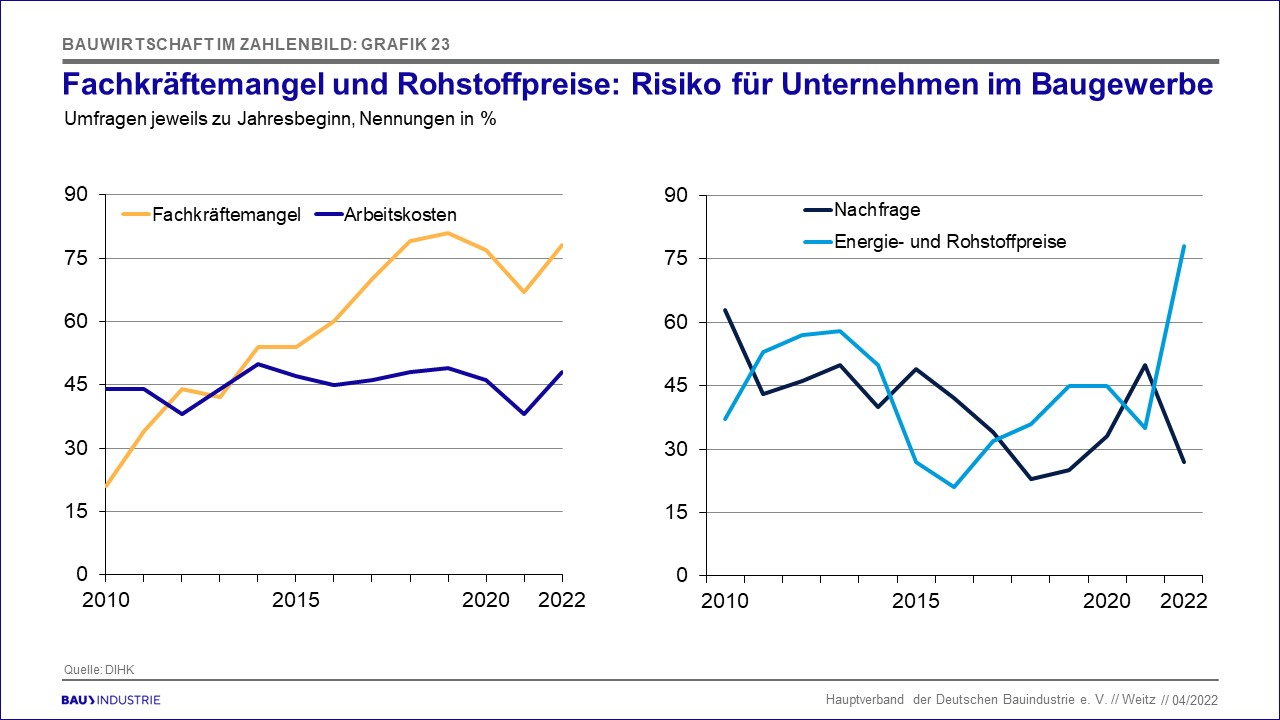
\includegraphics[width=0.7\columnwidth]{fig/Grafik_23.jpg}
    \caption{Während wirtschaftliches Risiko durch eine potentiell sinkende Nachfrage nach Bauafträgen und eventuell steigender Arbeitskosten unverändert blieben oder sogar als weniger relevant bewertet wurden, ist ein deutlicher Anstieg aufgrund des vorherrschenden Fachkräftemangels und der Energie- und Rohstoffpreise zu erkennen.}
    \label{fig:Fachkraeftemangel}
\end{figure}
Um dem entgegenzuwirken, etablieren sich bereits seit einigen Jahren Standards, um Bauprojekte digital zu begleiten.
Mit diesen soll gleichzeitig die Effizienz gesteigert, die Kommunikation zwischen den einzelnen Expertenteams vereinfacht, der Arbeitsplatz \glqq{}Baustelle\grqq{} sicherer gestaltet und ein resourcensparender Bau ermöglicht werden~\cite{BIMforHe12:online}\cite{Top10Ben31:online}.
Zusätzlich steigen mit der Zunahme an digitalen Informationen zu Bauprojekten, auch die Möglichkeiten diese ausführlicher zu analysieren, zu optimieren und an neue Technologien zu knüpfen.
Erst dadurch wurde das seit einigen Jahren erforschte Gebiet der \textit{Additiven Fertigung} von Gebäuden realisierbar.
Einige erfolgreiche Beispiele dafür sind in~\cite{AdditiveManufactoringDelgado},~\cite{AdditiveManufacturingUsingMobileRobots} und~\cite{Tankova2020} aufgezeigt und wurden etwa mit Beton druckenden Roboterarmen, mobilen Robotern oder aufgehängten Druckköpfen durchgeführt.
Dabei werden teils herkömmliche, teils speziell für die druckenden Roboter entwickelte Materialien verwendet~\cite{Tankova2020}.
Obwohl es mittlerweile viele Projekte zur Additiven Fertigung von Gebäuden gibt, haben diese oft den Nachteil der Nicht-Parallelisierbarkeit der druckenden Roboter und die daraus resultierende, vergleichsweise lange Bauzeit.
Auch die durch die Höhe der temporären Stützstrukturen (wie Kräne, Gerüste oder Aufhängungen) eingeschränkte Bauhöhe limitiert die Vielfalt der mit additiver Fertigung realisierbaren Projekte.
Diesen Einschränkungen soll nun mithilfe eines Schwarmes bodengebundener automoner Roboter, die gleichzeitig an dem Bauprojekt arbeiten können, entgegengewirkt werden.
Dabei sollen sich die Roboter auf den Mauern des Gebäudes selbst bewegen können, während sie diese errichten.
Im Gegensatz zur additiven Fertigung sollen die Roboter das Material nicht etwa drucken, sondern herkömmliche Bausteine verweden können.
In dieser Arbeit liegt der Schwerpunkt allerdings nicht auf der Entwicklung dieser Roboter, sondern auf dem Erarbeiten eines Vorgehens zur Berechnung von für Roboterschwärme geeigneten Bauplänen, ausgehend von 3D Modellen der Gebäude.
Dies stellt die Grundlage für nachfolgende Automatisierungsprojekte im Bereich der Bauindustrie dar.
Das Anfertigen der Modelle innerhalb eines 3D Editors ermöglicht nicht nur das Definieren geometrischer und physikalischer Eigenschaften eines Gebäudes in digitaler Form, sondern verschlankt zudem die Kommunikation zwischen Endnutzer und Architekturbüro oder ersetzt letzteres komplett.
Gleichzeitig macht diese Arbeit damit einen Schritt in Richtung des relativ neuen Trends der sogennanten Massenpersonalisierung, welcher als Nachfolgetrend zur Massenproduktion und als \glqq{}heilger Gral\grqq{} der Fertigung angesehen wird~\cite{MassCustomHolyGrail}.
Dieser Trend ist auch für die Bauindustrie interessant, denn auch hier schafft die Möglichkeit sämtliche Kundenwünsche an ein Produkt (oder in diesem Fall ein Gebäude) umzusetzen, ohne dafür spezielles Werkzeug herstellen oder Verfahren entwickeln zu müssen, neue Gewinnmöglichkeiten~\cite{Jensen2018}~\cite{Jensen2015}.
Dennoch existiert noch vergleichsweise wenig Forschung die teilweise schon etablierte Konzepte der Massenpersonalisierung aus der Fertigungsindustrie ebenfalls in der Bauindustrie zu erproben~\cite{Larsen2019}.
Darum soll in dieser Arbeit untersucht werden, in welcher Weise sich bereits vorhandene digitale Standards und Austauschformate dafür eigenen, individuelle Baupläne aus den 3D Plänen von Gebäuden zu generieren.
Die Baupläne können dabei aufgrund der Anbindung an einen frei verfügbaren 3D Editor nicht nur von Experten, sondern ebenfalls von Laien stammen.
So kann ein Endnutzer persönliche Wünsche selbst in das Modell integrieren.
Zudem wird nach einer Möglichkeit gesucht, die resultierenden Baupläne durch adaptive Regelsets an die jeweilige Situation anpassen zu können, denn unterschiedliche Bauprojekte besitzen oft unterschiedliche Eigenheiten und Prioritäten.
Diese Konzepte werden daraufhin anhand nachfolgender Fallstudien getestet.
\chapter{Fallstudien}\label{scenarios}
Anhand der nachfolgenden Fallstudien und Szenarien werden die dieser Arbeit zugrundeliegenden Konzepte veranschaulicht und auf Anwendbarkeit überprüft.
Dabei werden die Szenarien zunehmend komplexer, um auch das Zusammenspiel verschiedener Teilkonzepte zur Lösung einzelner Probleme zu verifizieren.
Abschließend wird für einige Szenarien untersucht wie Regeln erstens definiert und zweitens auf deren Ergebnisse angewandt werden können.
Damit sollen die ungeordneten Listen an Bausteinen, die das Ergebnis der Szenarien darstellen, so umsortiert werden, dass daraus ein schrittweise umsetzbarer Bauplan entsteht.

\section{Szenario 1}\label{scenarios:scenario1}
In diesem einleitenden Szenario werden anhand eines einfachen vierwändigen Turmes einige der Kernkonzepte geprüft.
Dabei werden sowohl die Modellierung des Turmes innerhalb eines Konstruktionsplaners, als auch die anschließende Bauplandeduktion thematisiert.
Insbesondere das Anwenden verschiedener Mauerwerksverbände soll die Flexibilität des erarbeiteten Vorgehens demonstrieren.
\subsection*{Beschreibung}
Das Modellieren des Gebäudes soll mit Hilfe der in Kapitel~\ref{basics} näher behandelten Technologien geschehen und enstpricht darum in seiner Struktur einem verbreiteten Industriestandard.
Der Turm besteht lediglich aus vier 20 Meter hohen Wänden, die einen einzigen Raum einschließen.
Es hat einen Grundriss von 10$\times$10 Metern.
Die Wände sollen daraufhin unter Anwendung folgender Mauerwerksverbände realisiert werden:
\begin{itemize}
  \item Einem Läuferverband mit einem Versatz von 50\% der Bausteinlänge.
  \item Einem Kopf/Binderverband.
  \item Einem Kreuzverband 
\end{itemize}
Da die beiden letzten Verbände bei gleichbleibendem Modul die Wanddicke verdoppeln, muss das Modell etwas angepasst werden, um nach wie vor den selben Grundriss aufzuweisen.
Als Basismodul wird ein Baustein mit den Maßen 2$\times$1$\times$0.5 Metern verwendet.
Das vereinfacht die Interpretation der generierten Lösungen.
Das dazugehörige Raster hat die Größe 1$\times$1$\times$0.5 Meter.

\subsection*{Problemstellungen}
Durch Lösen dieser Szenarien werden folgende Fragestellungen beantwortet:
\begin{itemize}
  \item In welcher Art muss das Basismodul vorliegen und wie kann es notfalls angepasst werden? 
  Denn oftmals werden an Wandenden oder Ecken Bausteine benötigt, die eine geringere Länge aufweisen.
  Dies entspricht in Realität dem Zerschneiden von Bausteinen.
  \item Wie können einem Algorithmus die verschiedenen Mauerwerksverbände sinnvoll vorgegeben werden?
  \item Wie können Eckbereiche gefunden und der jeweilige Mauerwerksverband auch an diesen Stellen passend angebracht werden ohne das Überbindemaß (siehe Kapitel~\ref{basics:Mauerwerksverband}) zu verletzen?
  \item Welche Informationen werden in den resultierenden Bauplan integriert?
\end{itemize}

\section{Szenario 2}\label{scenarios:scenario2}
Nun folgt ein Szenario das den Gegebenheiten eines realen Gebäudes eher entspricht.
Es soll ein Gebäude konstruiert werden, welches einen Innenraum, Fenster und Türen enthält.
Gleichzeitig wird das Modul stark verkleinert, sodass es den Maßen eines 4$\times$2 LEGO Steins entspricht (siehe Kapitel~\ref{basics:lego}).

\begin{figure}[ht]
  \centering
  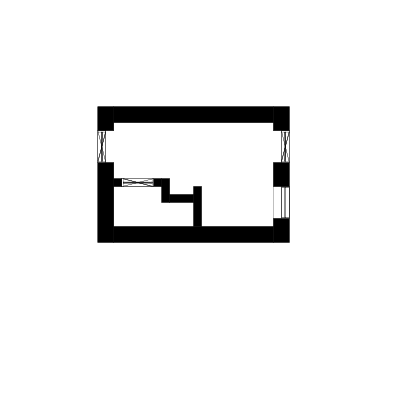
\includegraphics[width=0.505\columnwidth]{fig/scenario1_story_plan.jpg}
  \caption{Gebäudeplan des 3D Modells.}
  \label{fig:scenarios:Scenario1 Gebaeudeplan}
\end{figure}

\subsection*{Beschreibung}
Zu sehen ist der Plan eines einfachen Hauses mit einem Stockwerk.
Dieses besitzt eine Eingangstür, eine Terassentür neben einem Fenster und eine Tür, die das Badezimmer vom Hauptraum trennt.
Türen und Fenster stellen eine Herausforderung für den Planungsalgorithmus dar, da der Verlauf einer ansonsten durchgängigen Wand dadurch unterbrochen wird und Lücken aufweist.
Es gibt breite Außen- und dünne Innenwände.
Dafür müssen zwei Wandtypen definiert werden, die jeweils unterschiedliche Wanddicken vorgeben.
Diese entsprechen in ihren Maßen dem Raster, welches das \textit{LEGO System} vorgibt.
Breite Wände sollen zwei Noppen breit sein.
Daher hat deren Grundmodul Maße von 31.8$\times$15.8$\times$9.6 Millimetern mit einem Raster von 8$\times$8$\times$9.6 Millimetern.
Für die dünneren Innenwände soll eine Breite von einer Noppe verwendet werden.
Dies entspricht einem Grundmodul mit den Maßen 15.8$\times$7.8$\times$9.6 Millimetern mit einem gleichbleibenden Raster.
\begin{figure}[!ht]
  \centering
  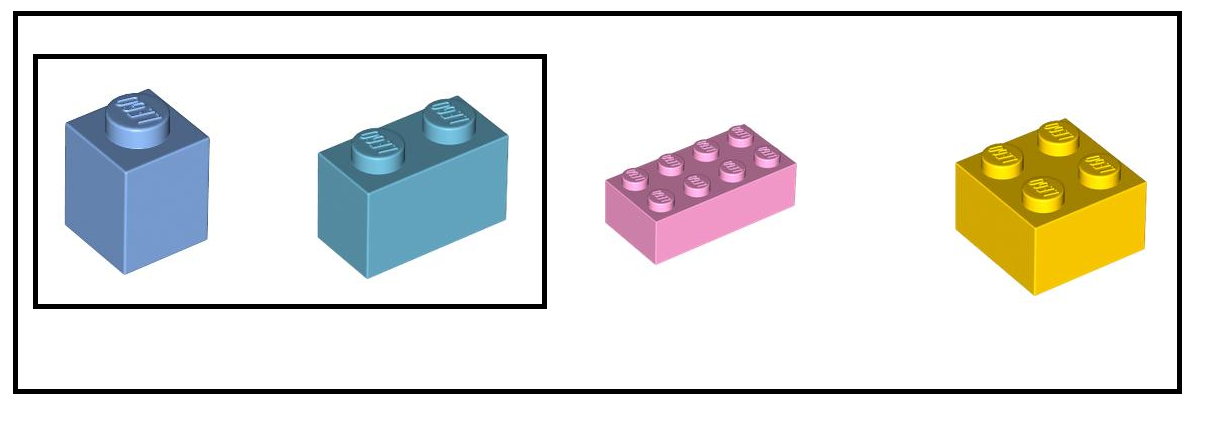
\includegraphics[width=0.6\columnwidth]{fig/scenario1_lego_set.png}
  \caption{LEGO Steintypen für die Innen- und Außenwände. (TODO Bild ist sehr hässlich)}
  \label{fig:Scenario1 Lego Set}
\end{figure}
Nicht nur die Abmessungen der Wände müssen in ein Raster fallen, auch deren Rotation wird in diesem Szenario auf 90\textdegree{} Schritte limitiert. 
Das stellt in diesem Fall eine vertretbare Enschränkung dar, da es ohnehin dem intuitiven Umgang mit LEGO Steinen und gleichzeitig dem Baustil der meisten einfachen Gebäuden entspricht.

\subsection*{Problemstellungen}
\begin{itemize}
  \item Wie können Öffnungen berücksichtigt werden?
  \item Stürze
  \item Verschiedene Wanddicken
  \item Übergänge zwischen verschiedenen Wanddicken
  \item T-Kreuzungen? Doch noch einbauen? Vlt die untere dünne wand dick machen?
\end{itemize}

\section{Scenario 3}\label{scenarios:scenario3}
Bauplandeduktion eines Gebäudemodells des KIT
\subsection*{Beschreibung}
Um das Konzept nicht nur an eigens modellierten Gebäuden zu evaluieren, werden zusätzlich externe Modelle herangezogen.
Dabei kann sich zum Beispiel an den Beispielprojekten des KIT bedient werden~\cite{KITSAMPLEHOUSE:online}.
TODO Bild von kleinem Hause
TODO überlegen ob eines der beiden riesendinger auch mal ran soll?
\subsection*{Problemstellungen}

\section{Scenario 4}\label{scenarios:scenario4}
Definition von Regelsets.
\subsection*{Beschreibung}
\subsection*{Problemstellungen}
\begin{itemize}
  \item Wie können Regelsets ohne Code vorgegeben werden? Also in welchem Format.
  \item In welcher Weise werden die Regeln dann angewendet etc?
\end{itemize}
\section{Related Work}
\subsection{3D Druck und Additive Fertigung von Gebäuden}
\subsection{Legeroboter}
\subsection{Materialien}
\subsection{Bausteine}
\subsection{Mauer detailing und das (3D) Bin Packing Problem}
TODO hinführen über Bin Packing hin zu "spezialfall" Wall detailing mit arbiträren Bausteinen und Eigenschaften (wie versetzen der ziegel)

TODO über bin packing schreiben, erklären paper suchen, lösungsansätze zu np hartem problem 

Xu Chengran et al. haben in ihrem Paper "Optimal brick layout of masonry walls based on intelligent evolutionary algorithm and building information modeling" verschiedene Optimierungsansätze aus dem Bereich des 2D Packaging Problems getestet \cite{Xu2021}.
%TODO was ist das für ein Problem? Zitat aus nem Paper finden!
Konkret wurden drei Algorithmen verwendet: Differential Evolution, Particle Swarm Optimization und Neighbourhood Field Optimization.
%TODO ergebnisse vergleichen und eines davon hervorheben, welches ich evtl selbst einbau
Außerdem wird ein drei-phasiges Vorgehen vorgeschlagen: Data collection, Brick layout und Data Output.
%TODO das vmtl einfach auch so aufziehen. Mauern aus modell extrahieren mit geometrischen infos, optimieren und iwie rausballern
Dieses Vorgehen eignet sich auch für das Finden von Bausteinkonfigurationen in dieser Arbeit, da zuerst alle relevanten geometrischen Daten (in diesem Fall Wände, Fenster, Türen usw.) aus dem 3D Modell gesammelt werden müssen, bevor das Detailing stattfinden kann.
Nach dem Optimieren der Bausteinkonfiguration muss das Ergebnis ebenfalls in ein Format gebracht werden, das für die folgenden Schritte verwendet und eventuell auch dem Nutzer angezeigt werden kann.


Soft items: https://arxiv.org/abs/2206.15116

Irregular Shaped items: https://link.springer.com/content/pdf/10.1631/FITEE.1400421.pdf

"Parametric Blockwall-Assembly Algorithms for the Automated Generation of Virtual Wall Mockups Using BIM"

% https://academy.ifcopenshell.org/posts/using-ifcopenshell-and-pythonocc-to-generate-cross-sections-directly-from-an-ifc-file/
% https://blenderbim.org/docs-python/ifcopenshell-python/geometry_processing.html
%https://academy.ifcopenshell.org/posts/using-ifcopenshell-and-pythonocc-to-construct-new-geometry/

\chapter{Grundlagen}\label{basics}
Zunächst wird für diese Arbeit ein geeignetes Speicherformat für 3D Modelle von Gebäuden benötigt.
Um den Bau von Gebäuden zu automatisieren, ist es notwendig die Domäne \textit{Gebäude} möglichst vollständig digital abbilden zu können. 
Hilfreich ist dabei, wichtige Daten über bestimmte Bestandteile des Gebäudes direkt in das Modell zu integrieren, auf Basis derer etwa Kostenberechnungen durchgeführt oder Materialmengen herausgefunden werden können.
Da diese Informationen oft von Experten verschiedener Fachbereiche (etwa aus den Bereichen der Architektur, des Bauwesens oder der Statik) stammen, muss das Format sehr flexibel und im besten Fall auch zeitgleich bearbeitbar sein.
Dafür werden seit dem Jahr 2000 die \textit{Industry Foundation Classes} (IFC) von buildingsmart entwickelt, deren Anwendung im internationalen Bauwesen mittlerweile weit verbreitet ist~\cite{Industry61:online}.


\section{Industry Foundation Classes}\label{basics:ifc}
In der Spezifikation des Standards selbst, wird dieser wie folgt beschrieben:
\glqq{}Die Industry Foundation Classes (IFC) sind ein offener internationaler Standard für Daten des Building Information Model (BIM), welche zwischen Softwareanwendungen ausgetauscht, gemeinsam genutzt und von den verschiedenen Akteuren der Bauindustrie und des Gebäudemanagements verwendet werden. 
Der Standard enthält Definitionen für Daten, die für die Lebenszyklen von Gebäude- und Infrastrukturarbeiten erforderlich sind. 
Die bis jetzt in die IFC aufgenommenen Infrastrukturtypen umfassen Brücken, Straßen, Eisenbahnen, Wasserstraßen und Hafenanlagen\grqq{} (aus dem Englischen)~\cite{IFCScope:online}. 
Eine frühere Version des IFC Standards ist unter der Bezeichnung ISO 16739 registriert (siehe~\cite{ISOISO1694:online}).
Da die IFC aber nach wie vor kontinuierlich weiterentwickelt werden, wird in dieser Arbeit die derzeit neueste Version verwendet.
Diese ist die IFC Spezifikation 4.3.1.0~\cite{IFC4310Spezification:online}.
Das verbreitetste Austauschformat für IFC ist das Step Physical File Format, welches im ISO 10303 Teil 21 registriert ist~\cite{ISO_Step:online}.
Zudem gibt es speicherreduzierte Formate wie ifcZip oder für Menschen lesbarere Formate wie ifcXML~\cite{Industry93:online}\cite{IFCForma28:online}\cite{BIM_handbook_AEC_XML_SCHEMAS}.

\subsection{IFC 4.3.1.0 Aufbau}
Im Grunde definieren die \textit{Industry Foundation Classes} eine Vielzahl an Klassen, die in einer komplexen Hierarchie angeordnet den Grundstock des Datenmodells bilden.
Diese sind anfangs abstrakte Konzepte, die sich mit zunehmender Tiefe in der Hierarche konkretisieren.
\begin{figure}[ht]
    \centering
    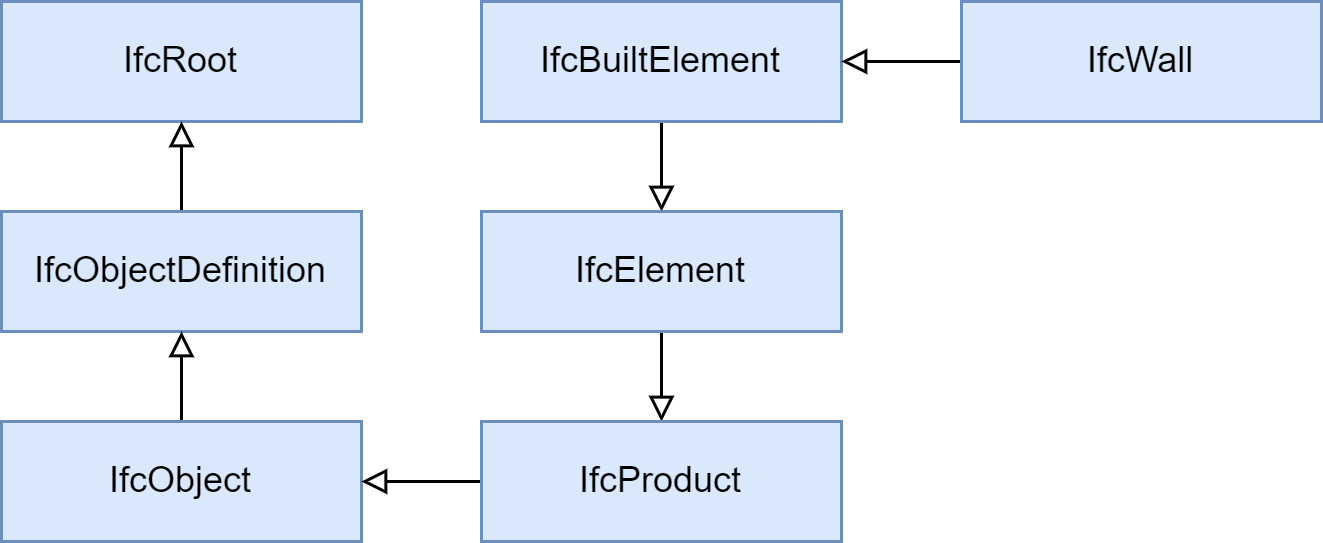
\includegraphics[width=0.6\columnwidth]{fig/Hierarchie_IfcWall_300.drawio.png}
    \caption{Klassenhierarchie am Beispiel der Klasse \textit{IfcWall}}
    \label{fig:IfcWall_Hierarchie}
\end{figure}
Da sich diese Arbeit zum größten Teil mit aus Wänden bestehenden Gebäuden befasst, wird nachfolgend die Klasse \textit{IfcWall} wiederholt als Beispiel herangezogen.
Der für diese Klasse relevante Ausschnitt aus der Klassenhierarchie ist in Abbildung~\ref{fig:IfcWall_Hierarchie} dargestellt.
Objekte werden von dem Standard in Relation zueinander gestellt, um komplexere Zusammenhänge darzustellen.
In Abbildung~\ref{fig:IFC_Relationships} erkennt man den Zusammenhang zwischen einem Objekt des Types \textit{IfcWall}, des Stockerwerks, welches diese Wand referenziert und wiederum selbst Teil eines \textit{IfcBuildings} ist, bis hin zur obersten Komponente eines Ifc Projektes, dem gleichnamigen \textit{IfcProject}.

\begin{figure}[h]
    \centering
    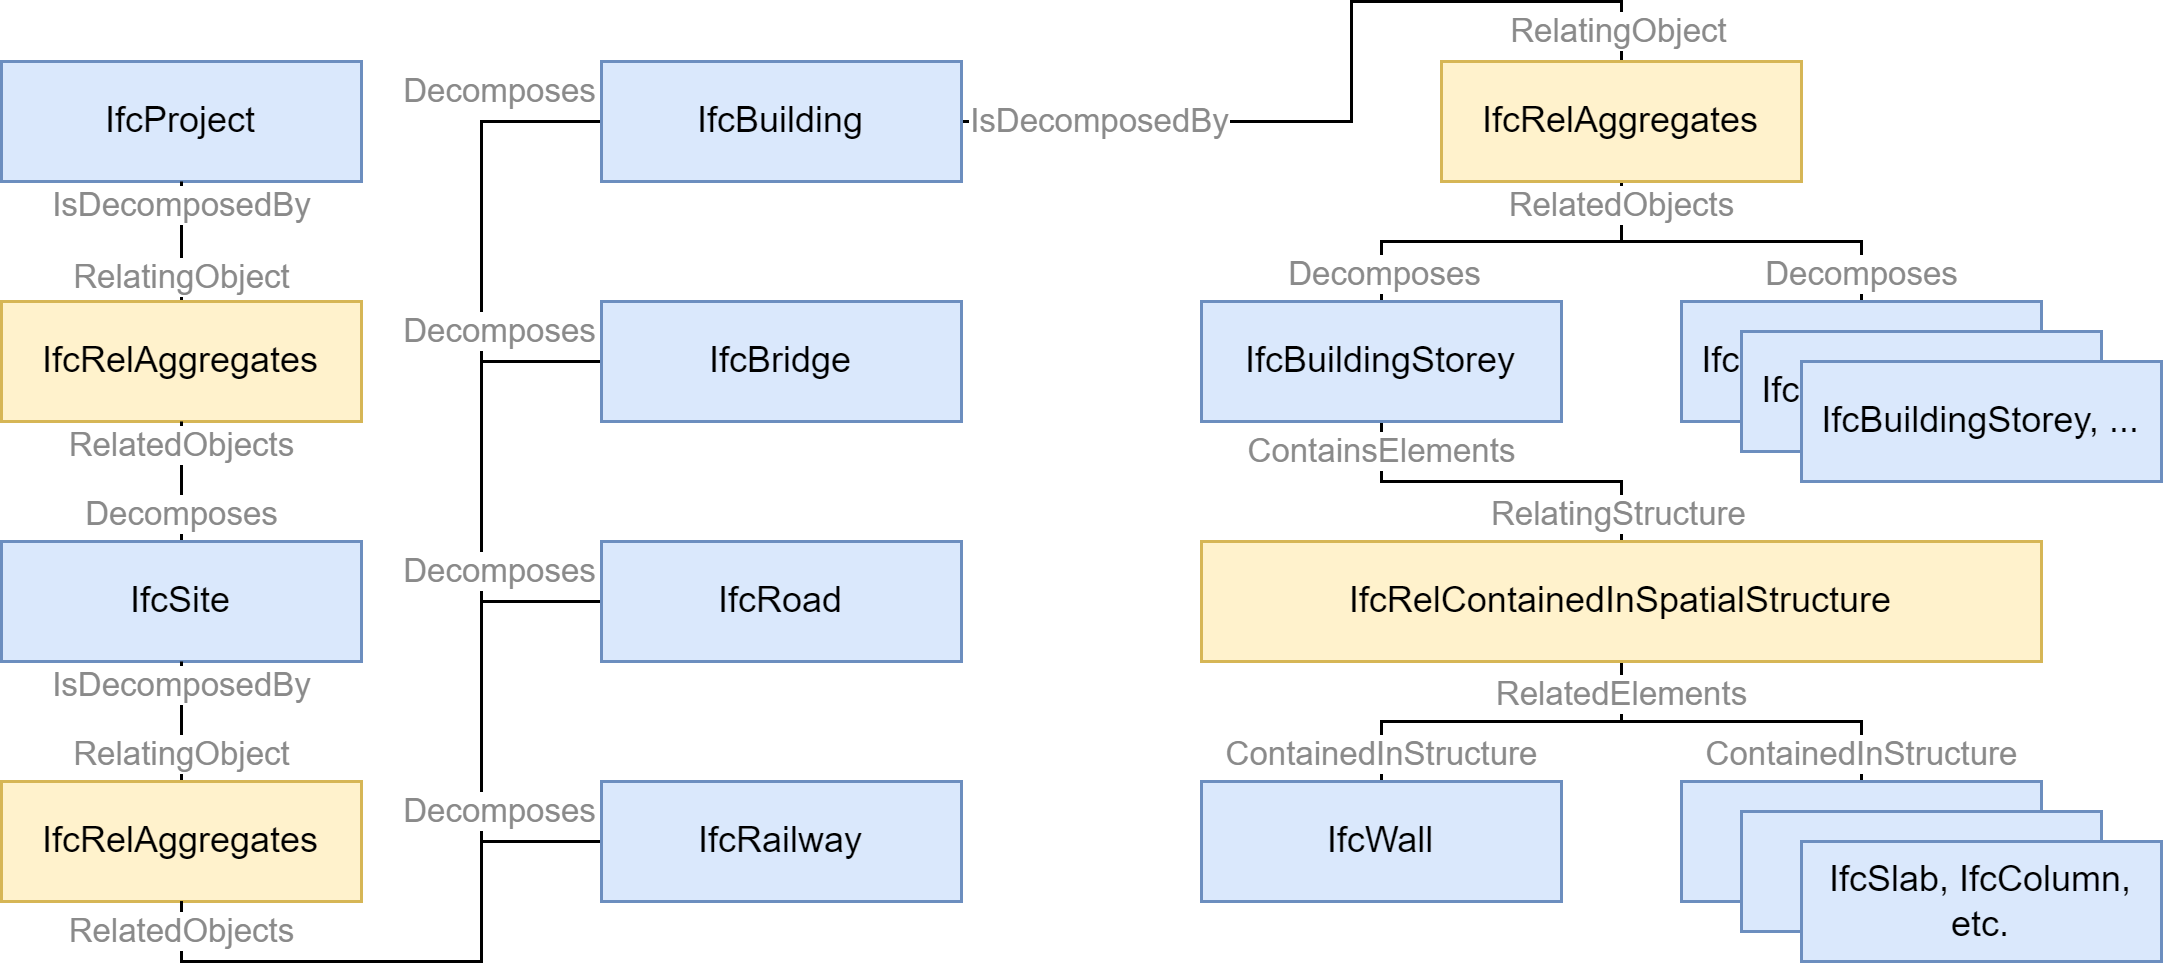
\includegraphics[width=0.9\columnwidth]{fig/IFC_Relationships_300.drawio.png}
    \caption{Relation der IfcWall und einem \textit{IfcProject}}
    \label{fig:IFC_Relationships}
\end{figure}

\subsection{IfcPropertySets und IfcQuantitySets}\label{basics:ifc_properties}
Mit dem Erweitern des Gebäudemodells um möglichst viele Informationen, schafft man einen detailierten digitalen Zwilling, der neben der bloßen Darstellung des Gebäudes als 3D Modell zusätzlich die Untersuchung auf andere Eigenschaften ermöglicht.
Dazu zählen zum Beispiel eine präzisere Kosten- und Zeitschätzung, Sicherheitsaspekte und Emissionen eines Bauvorhabens~\cite{Industry93:online}~\cite{Ding2014}. 
Dies ist mithilfe von \textit{IfcPropertySets} und \textit{IfcQuantitySets} umsetzbar, welche Objekten oder Objekttypen angehängt werden können.
Dabei werden IfcQuantitySets vorwiegend dazu verwendet numerische Werte zu geometrischen oder physikalischen Eigenschaften auszudrücken.
IfcPropertySets dienen hingegen dazu bestimmten Objekten oder Objekttypen mit sämtlichen nicht numerischen Werten zu annotieren.
Beispiele dafür sind etwa Material oder Farbe eines bestimmten Objekts.
Die Verwendung der Bezeichnung \textit{Set} rührt daher, dass diese Informationen in einer Baumstruktur vorliegen und demnach verschachtelt sein können.
Es gibt zu vielen Klassenbeschreibungen des IFC Standards vordefinierte PropertySets.
Das hilft dabei wichtige Informationen zu bestimmten Objekttypen einheitlich angeben zu können.
Im Falle des \textit{IfcWallType} existiert beispielsweise das PropertySet mit dem Namen \textit{Pset\_WallCommon}~\cite{IFC4310PSetWallCommon:online}.
Darin können die Ersteller von neuen WallTypes unter anderem Informationen über Brennbarkeit, thermisches Verhalten oder Akustik hinterlegen.
Bei Erstellen einer IfcWall-Instanz aus einem bestimmten WallType werden die damit verbundenen Property- und QuantitySets automatisch daran angehängt, sodass jedes Objekt relevante Informationen über sich selbst bereithält.

\subsection{Positionierung von \textit{IfcProducts}}
%https://ifc43-docs.standards.buildingsmart.org/IFC/RELEASE/IFC4x3/HTML/concepts/Product_Shape/Product_Placement/Product_Local_Placement/content.html
Die Platzierung eines \textit{IfcProducts} wird durch eine Verkettung relativer Transformationen ausgehend vom \textit{IfcProduct}, über sätmliche Strukturen, die dieses Objekt enthalten, bis hin zur \textit{IfcSite} realisiert~\cite{IFCPlatzierung}.
Diese Hierarche kann der Abbildung~\ref{fig:IFC_Relationships} entnommen werden.
Um die globale Position eines \textit{IfcProducts} zu erhalten, müssen die relativen Transformationen miteinander verrechnet werden.
Der IFC Standard unterstützt zudem die Möglichkeit Positionierungen anhand eines Rasters oder mithilfe des sogennanten \textit{linear placements} anzugeben.

\subsection{IfcOpeningElement}
\label{basics:IfcOpeningElement}
Neben Wänden stellen Fenster und Türen wichtige Elemente eines Gebäudes dar.
Diese sind ebenfalls Teil der Klassen des IFC Standards.
Objekte des Typs \textit{IfcOpeningElement} dienen dazu die notwendigen Lücken in einer Wand zu definieren in die später eine Tür oder ein Fenster eingebaut werden soll.
In der Dokumentation wird dies wie folgt formuliert (aus dem Englischen): \glqq{}[Das IfcOpeningElement] stellt eine Lücke in jedem Element dar, das eine physische Manifestation hat\grqq{}~\cite{IFC4310OpeningElement:online}.
Es gibt zwei Arten an IfcOpeningElement, je nachdem ob die Öffnung durch die gesamte Breite eines Objektes reicht oder nicht. 
Folglich entsteht dadurch eine Unterscheidung zwischen Nischen und tatsächlichen Öffnungen, wobei nur letztere im Zusammenhang mit Fenstern oder Türen Sinn ergibt.
TODO: Diagramm zwischen IFCWall und IfcOpeningElement.

\section{IFC for Blender}\label{basics:blender}
\subsection{Blender}
Blender ist eines der beliebtesten Open Source Programme zur Modellierung von 3D Modellen und Animationen~\cite{blendero56:online}.
Eine umfangreiche Python API erlaubt es Blender durch sogenannte Addons an die eigenen Bedürfnisse anzupassen~\cite{PythonWebsite:online}~\cite{BlenderPythonAPI:online}.
Aufgrund dessen existiert auch eine Vielzahl an freien Erweiterungen \textendash{} unter anderem auch eine Integration von IFC Projekten.

\subsection{blenderbim}
Neben kommerziellen Produkten wie etwa revit von autodesk zur Modellierung von IFC Modellen, gibt es auch für Blender ein freies Plugin, um IFC Modelle zu erstellen~\cite{RevitSof26:online}~\cite{BlenderB43:online}.
Dieses Plugin ermöglicht es neben dem bloßen Designen des Gebäudes in kurzer Zeit z.B. detailierte Zeichnungen verschiedener Perspektiven herauszuarbeiten, die z.B. von Bauingeneuren verwendet werden können, um einzelne Stockwerke oder Verkabelungen zu planen.
Blenderbim selbst kapselt unter anderem die Open Source Python Bibliothek \textit{IfcOpenShell}, sodass diese in der Blender Laufzeitumgebung zur Verfügung steht \cite{IFCOpenShell:online}.

\subsection{IfcOpenShell}\label{basics:ifcopenshell}
\begin{lstlisting}[label={basics:ifcopenshell_sample_code}, language=Python, caption=Beispielprogramm zur Extraktion bestimmter Daten einer IFC Datei und Generierung eines Meshes aus deren geometrischen Representationen.]
import ifcopenshell
from ifcopenshell import geom
from stl import mesh, Mode
import numpy as np

settings = ifcopenshell.geom.settings()
settings.set(settings.USE_WORLD_COORDS, True)

ifc_file = ifcopenshell.open("model.ifc")
products = ifc_file.by_type("IfcProduct")
meshes = []

for product in products:
    if product.Representation and product.is_a("IfcWall"):
        shape = ifcopenshell.geom.create_shape(settings, product)
        vertices = np.array(shape.geometry.verts).reshape((-1, 3))
        edges = np.array(shape.geometry.edges)
        faces = np.array(shape.geometry.faces).reshape((-1, 3))

        m = mesh.Mesh(np.zeros(faces.shape[0], dtype=mesh.Mesh.dtype))
        for i, f in enumerate(faces):
            for j in range(3):
                m.vectors[i][j] = vertices[f[j], :]
        meshes.append(m)

# Create the combined mesh
combined = mesh.Mesh(np.concatenate([m.data for m in meshes]))
combined.save('model.stl', mode=Mode.ASCII)
\end{lstlisting}

IfcOpenShell ist eine frei verfügbare Bibliothek, die es erleichtert mit Daten im IFC Format zu arbeiten.
Sie bietet unter anderem eine Python API an und ist wie bereits erwähnt ein Teil des Blender Addons blenderbim.
Natürlich ist es dennoch möglich diese Bibliothek auch ohne Blender zu verwenden.
In Listing~\ref{basics:ifcopenshell_sample_code} ist ein kurzes Beispiel eines Programmes gegeben, das in einer IFC Datei alle Objekte des Typs IfcWall ausfindig macht und dessen geometrische Representation in ein herkömmliches Mesh konvertiert.
Damit existiert ein intuitiver Zugang zu den Daten von IFC Dateien.

\section{Building Information Modeling}\label{basics:bim}
Ein weiterer Punkt, der für die Verwendung von IFC spricht ist das sogenannte \textit{Building Information Modeling} (BIM)~\cite{Building41:online}.
Ein Definitionsvorschlag lautet wie folgt: \glqq{}BIM ist definiert als der Einsatz von Informations- und Kommunikationstechnologien zur Verschlankung der Prozesse im Lebenszyklus von Gebäuden, um eine sicherere und produktivere Umgebung für die Bewohner zu schaffen, die Umwelt so wenig wie möglich zu belasten und die Effizienz der Betriebsabläufe für die Eigentümer während des gesamten Lebenszyklus des Gebäudes zu erhöhen\grqq{} (Übersetzt aus dem Englischen)~\cite{Microsof51:online}.
Zum Lebenszyklus eines Gebäudes gehören etwa anfangs das Planen und Designen, später das Bauen, das Verwenden und Instandhalten und nach eventuellen Renovierungen das Abreißen.
BIM kommt in all diesen Phasen zum Tragen und erleichtert diese Prozesse durch Anbieten einer einheitlichen Schnittstelle für alle am Infrastrukturbau und -management beteiligten Personen.
Zusätzlich ermöglicht BIM eine exakte Dokumentation des Geschehens in sämtlichen Phasen des Bauwerks, was unter anderem zu einer genaueren Zeit- und Kostenplanung führt~\cite{Ding2014}.
Auch Verantwortlichkeiten sind Teil von BIM, was zu einer erhöhten Produktivität beiträgt.
Um nun das Zusammenarbeiten der unterschiedlichen Fachbereiche zu erleichtern, gibt es sogennante BIM-Server auf welchen mehrere Arbeitende synchron an einem Projekt arbeiten können, während sie jeweils die für ihren Aufgabenbereich passende Ansicht vor sich haben.
BIM-Server unterstützen zusätzlich eine Versionierung des Fortschritts an einem Projekt.

In einem Gespräch mit einem Ingeneur aus dem Bereich \glqq{}Energysystemtechnik\grqq{} kam zur Sprache, dass viele Bereiche von BIM noch nicht ganz Einzug in Deutschland gefunden haben.
Eben jene \glqq{}Kollaboration über einen BIM-Server mit Änderungsmanagement etc. [sei] (noch) nicht üblich, da noch nicht alle Beteiligten dazu in der Lage sind. Vor allem Bauherren, Architekten und Baufirmen können es nicht\grqq{}.
Weiter sei \glqq{}auch unklar, wer für falsche Angaben haftet und wer die Konsistenz aller Daten gewährleistet\grqq{}.
Auf der anderen Seite sei \glqq{}das im BIM festegelegte Datenformat IFC das Maß der Dinge und auch bei uns so in Verwendung\grqq{}.
Auch das Einpflegen \glqq{}ergänzende[r] Bauteilinformationen (z.B. zu Gewicht, Dämmwert, Recyclebarkeit, CO2 Fußabdruck, etc.)\grqq{} finden Einsatz und sind Teil seines Alltags.
Für ihn wichtig ist ebenfalls der Betrieb des Gebäudes.
Hier unterstützt BIM, indem sämtliche Teile der Installationen in einem Gebäude, wie z.B Fensterdichtungen, Kabel, Rohre, Sicherungen oder eine Umwälzpumpe individuelle Teilenummern zugewiesen bekommen, hinter welchen alle Daten wie etwa Hersteller, Bestellnummern, Lebensdauer, Wartungshistorie oder Entsorgungsnachweise vermerkt sind.
Dies wurde allerdings \glqq{}angesichts der Realität der Handwerker und Gebäudenutzer für völlig unrealisitsch und auch etwas over-engineered\grqq{} eingestuft.
Trotzdem sei \glqq{}BIM [\ldots] das große Ding in der Bauwelt und der einzige echte Standard\grqq{}.

\section{opensourcebim}
Während es vorwiegend kommerzielle Produkte gibt, die Unternehmen das Arbeiten mit BIM ermöglichen, exisitiert auch hier eine aktive Open Source Bewegung.
Unter dem Namem \glqq{}The open source BIM collective\grqq{} oder kurz \glqq{}opensourceBIM\grqq{} werden derzeit um die 70 Repositories betrieben.
Darin enthalten sind unter anderem ein BIM-Server inklusive verschiedener Clients für Endanwender auf unterschiedlichen Systemen und Werkzeuge, die es erleichtern den IFC Files zu arbeiten~\cite{Theopens96:online}.
Ein kurzer Test hat gezeigt, dass die in Blender modellierte IFC Files tatsächlich über einen \glqq{}Anzeige-Client\grqq{}, der mit einem lokal gehosteten BIM-Server verbunden ist, angezeigt werden können.
Obwohl die Verwendung des BIM-Servers für diese Arbeit nicht notwendig ist, besteht die Option diesen künftig mit in den Workflow zu integrieren, da damit auch das simultante Arbeiten an einem IFC File möglich ist, was in Blender nur teilweise und mit dem Einsatz von Plugins ermöglicht wird.
Das stellt einen Praxisbezug zum aktuell verwendeten Stand dieser Technologien her, was in der oftmals konzeptionellen Natur der Forschung nicht immer der Fall ist.
Wie auch Blender untertützt BIM-Server das Einbinden von eigenen Plugins, sodass eine Erweiterung um neue Funktionalität möglich ist.
Die Plugins werden in Java geschrieben.
Der Server bietet aber auch eine REST Schnittstelle an, um Clients in anderen Sprachen anzubinden.

\section{Mauerwerksbau}
\label{basics: Mauerwerksbau}
Der Mauerwerksbau ist eine Art des Massivbaus, bei welchem Natur- oder Formsteine aufgeschichtet werden, um Wände beziehungsweise Mauern zu errichten.
Eine derart erbaute Wand besteht demnach aus (Bau)-Steinen und den dazwischen entstehenden Fugen.
Mörtel ist dabei nicht zwangsläufig notwendig.
Man spricht von trocken versetzten Steinen oder einer Trockenmauer, wenn darauf verzichtet wird.
Heutzutage wird fast ausschließlich mit quaderförmigen Formsteinen gebaut.
Zur Beschreibung solcher Formsteine existieren zwei relevante Größen.
Die eine ist das sogenannte \textit{Baunennmaß}, mit dem die tatsächliche Größe des Steins angegeben wird.
Die andere das \textit{Baurichtmaß}, das sich aus Baunennmaß und dem Fugenmaß zusammensetzt.

\subsection{Maßsysteme}
Als Maßsystem bezeichnet man das Vorgeben der Größen von Bausteinen anhand eines konkret definierten (Grund-)Moduls.
Zwei in Deutschland populäre Grundmodule sind zum einem das \textit{ISO-2848-Basismodul} mit Länge 100mm und zum anderen der Achtelmeter, verankert in der \textit{DIN 4172 Maßordnung im Hochbau}~\cite{ISO2848}\cite{DIN417224}.
Letzteres bezeichnet man daher auch als das oktametrische Maßsystem.
Nachfolgend wird auf dieses Maßsystem näher eingegangen.

\subsubsection*{Oktametrisches Maßsystem}
Baurichtmaße sind gemäß dem oktametrischen Maßsystem immer ein Vielfaches von \(12,5 cm\) (das entspricht \(1/8 m\)) und nach der Norm aber mindestens \(6.25cm\).
Dies gilt sowohl für Länge und Breite als auch für die Höhe der Steine.
Das System ist in der \textit{DIN 4172 Maßordnung im Hochbau} geregelt und ist ein fest definiertes Grundmaß für das Bauwesen in Europa~\cite{DIN417224}.
\begin{figure}[ht]
    \centering
    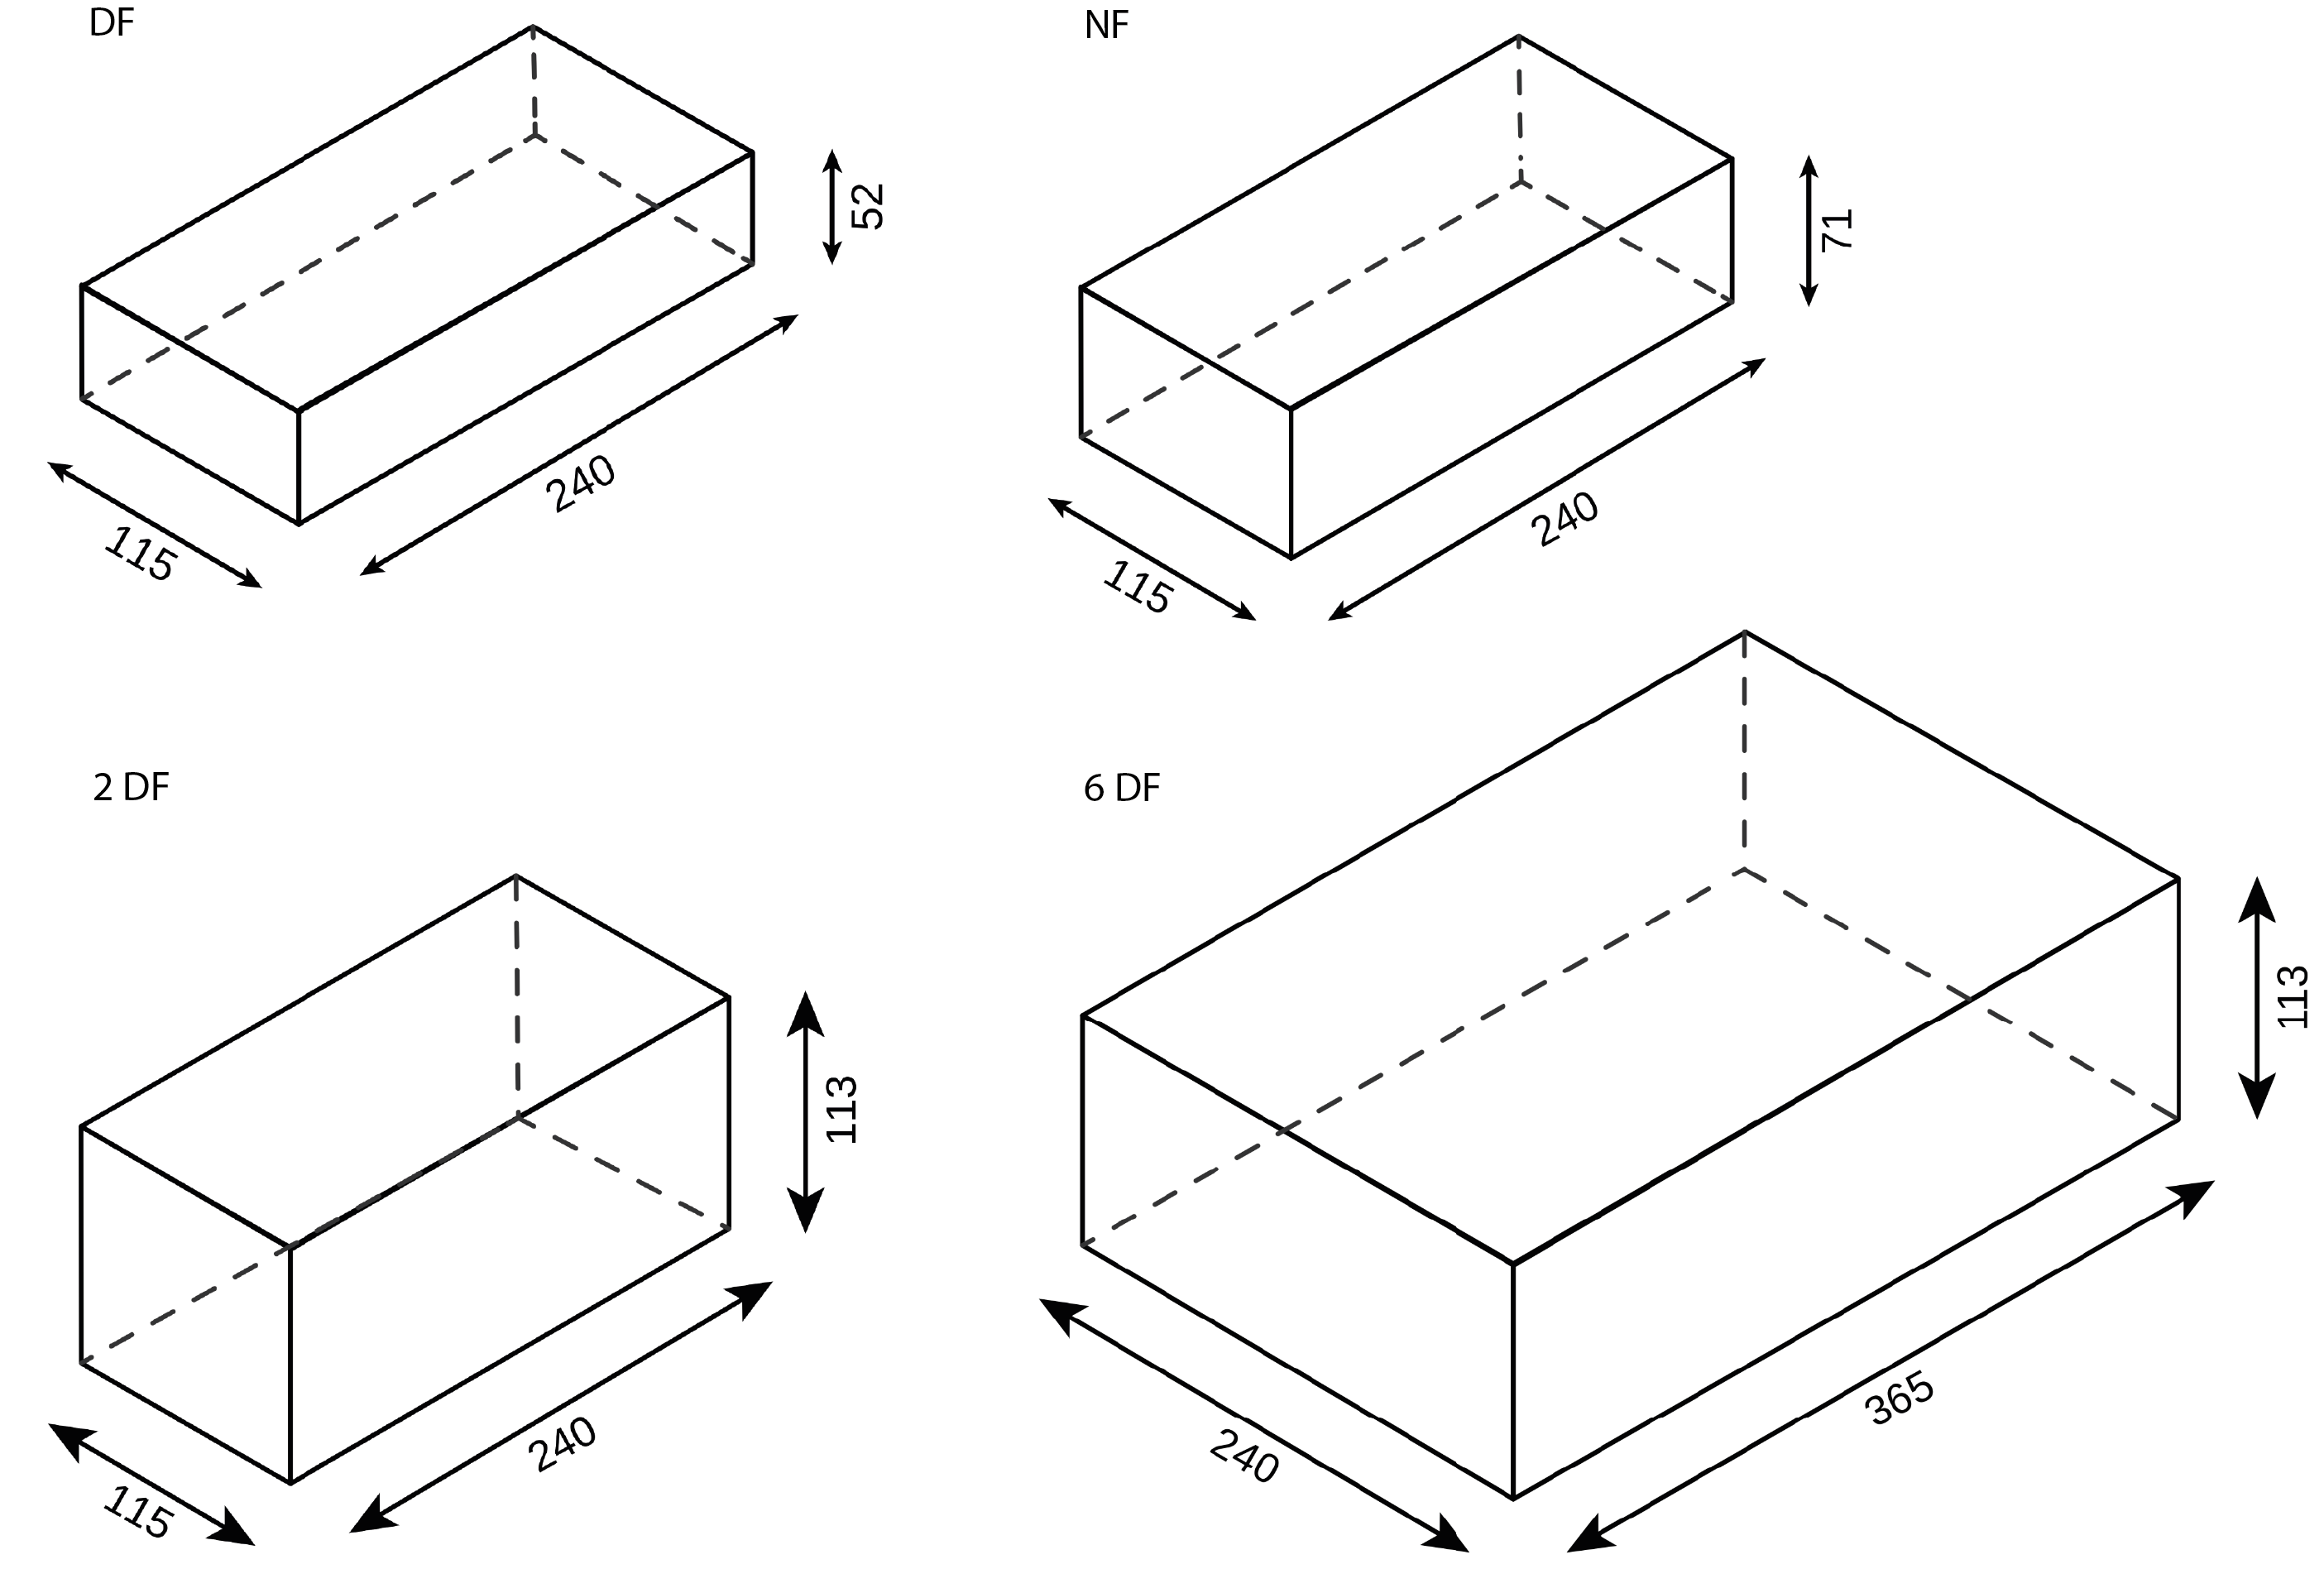
\includegraphics[width=0.8\columnwidth]{fig/Ziegelsteinformate DF NF 2DF 6DF.png}
    \caption{Darstellung verschiedener Steinformate nach DIN 4172 (Baunennmaß in Millimetern)~\cite{Steinfor38:online}}
    \label{fig:basics:Steinformate}
\end{figure}
\begin{figure}[hb]
  \centering
  \includegraphics[width=0.8\columnwidth]{fig/Oktametrische Maßordnung.png}
  \caption{Besondere Eigenschaften der oktametrischen Maßordnung~\cite{Moro2021}}
  \label{fig:basics:OktametrischeMassordnung}
\end{figure}
Daraus gehen insbesondere folgende zwei Formate für Ziegelsteine hervor:
Das Normalformat (NF) mit \(240\times115\times71 mm\) und das Dünnformat (DF) mit \(240\times115\times52 mm\) (Länge$\times$Breite$\times$Höhe)~\cite{Moro2021}.
Alle anderen Formate werden mithilfe dieser beiden Grundsteine angegeben.
So sind zum Beispiel die in Abbildung~\ref{fig:basics:Steinformate} gezeigten 2 DF und 6 DF Steine eine Kombination aus mehreren Steinen im Dünnformat.
Dabei sieht die Norm ein Fugenmaß von \(10 mm\) für Stoßfugen (vertikal) und \(12 mm\) for Lagerfugen (horizontal) vor.
Für Systeme, die eine schmalere oder keine Fuge benötigen, werden entsprechend größere Steine hergestellt, um der Maßordnung weiterhin zu entsprechen.
Durch Einhalten eines Systems ist man zusätzlich in der Lage Türen und Fenster an die daraus entstehenden Öffnungsgrößen anzupassen und vermeidet dadurch zeitaufwendiges, nachträgliches Anpassen.
Da Höhe, Breite und Länge der Steine zusammen mit den dazwischenliegenden Fugen aufgrund des Maßsystems jeweils Vielfache voneinander sind, ergeben sich viele Möglichkeiten zur Aufschichtung und Aneinanderreihung der Bausteine.
Einige davon sind in Abbildung~\ref{fig:basics:OktametrischeMassordnung} zu sehen und sind gleichzeitig Beispiele für einen sogenannten \textit{Mauerwerksverband}.

\subsection{Mauerwerksverband}
\label{basics:Mauerwerksverband}
Als Mauerwerksverband bezeichnet man bestimmte, gleichmäßige Anordnungen von Mauersteinen, um einen homogenen Mauerwerkskörper zu erreichen~\cite{Mauerwer39:online}.
Damit kann eine gleichmäßige Kraftverteilung innerhalb der Mauer gewährleistet werden.
Eine wichtige Rolle nimmt dabei das Überbindemaß ein, welches die Mindestüberlappung von Mauersteinen aus zwei Schichten der Mauer vorgibt.
Für das planmäßige Überbindemaß \(l_{ol}\) gilt für übliche Mauersteine mit Schichthöhen 
\(h_{u} \leq 249 mm\) 
nach DIN EN 1996-1-1: 
\(l_{ol} \geq 0,4h_{u} \geq 45 mm\)
~\cite{Bemessun72:online}\cite{DIN_EN_1996_1_1}.
Zudem wird darin die Mindestwanddicke für tragendes Mauerwerk, \glqq{}sofern aus Gründen der Standsicherheit, der Bauphysik oder des Brandschutzes nicht größere Dicken erforderlich sind\grqq{}~\cite{Bemessun72:online}, auf 
\(t_{min} = 115 mm\) 
festgelegt~\cite{DIN_EN_1996_1_1}.
Dies ist, wie in Abbildung~\ref{fig:basics:Steinformate} zu sehen, exakt die Breite der kleinsten Ziegelformate NF und DF.
Man unterscheidet zwei Arten von Mauerwerk: das Einsteinmauerwerk und das Verbandsmauerwerk.
Wie schon dem Namen zu entnehmen, handelt es sich beim Einsteinmauerwerk und ein Mauerwerk, bei welchem die Wanddicke der Steindicke entspricht.
Hier muss das Überbindemaß lediglich über die Wandlängsrichtung eingehalten werden.
Bei Verbandsmauerwerk gilt dies zusätzlich für die Wandquerrichtung~\cite{05maurer1:online}.
Einige Beispiele sind in Abbildung~\ref{fig:basics:verbaende} zu sehen.
\begin{figure}[htb]
  \begin{subfigure}[b]{0.5\columnwidth}
    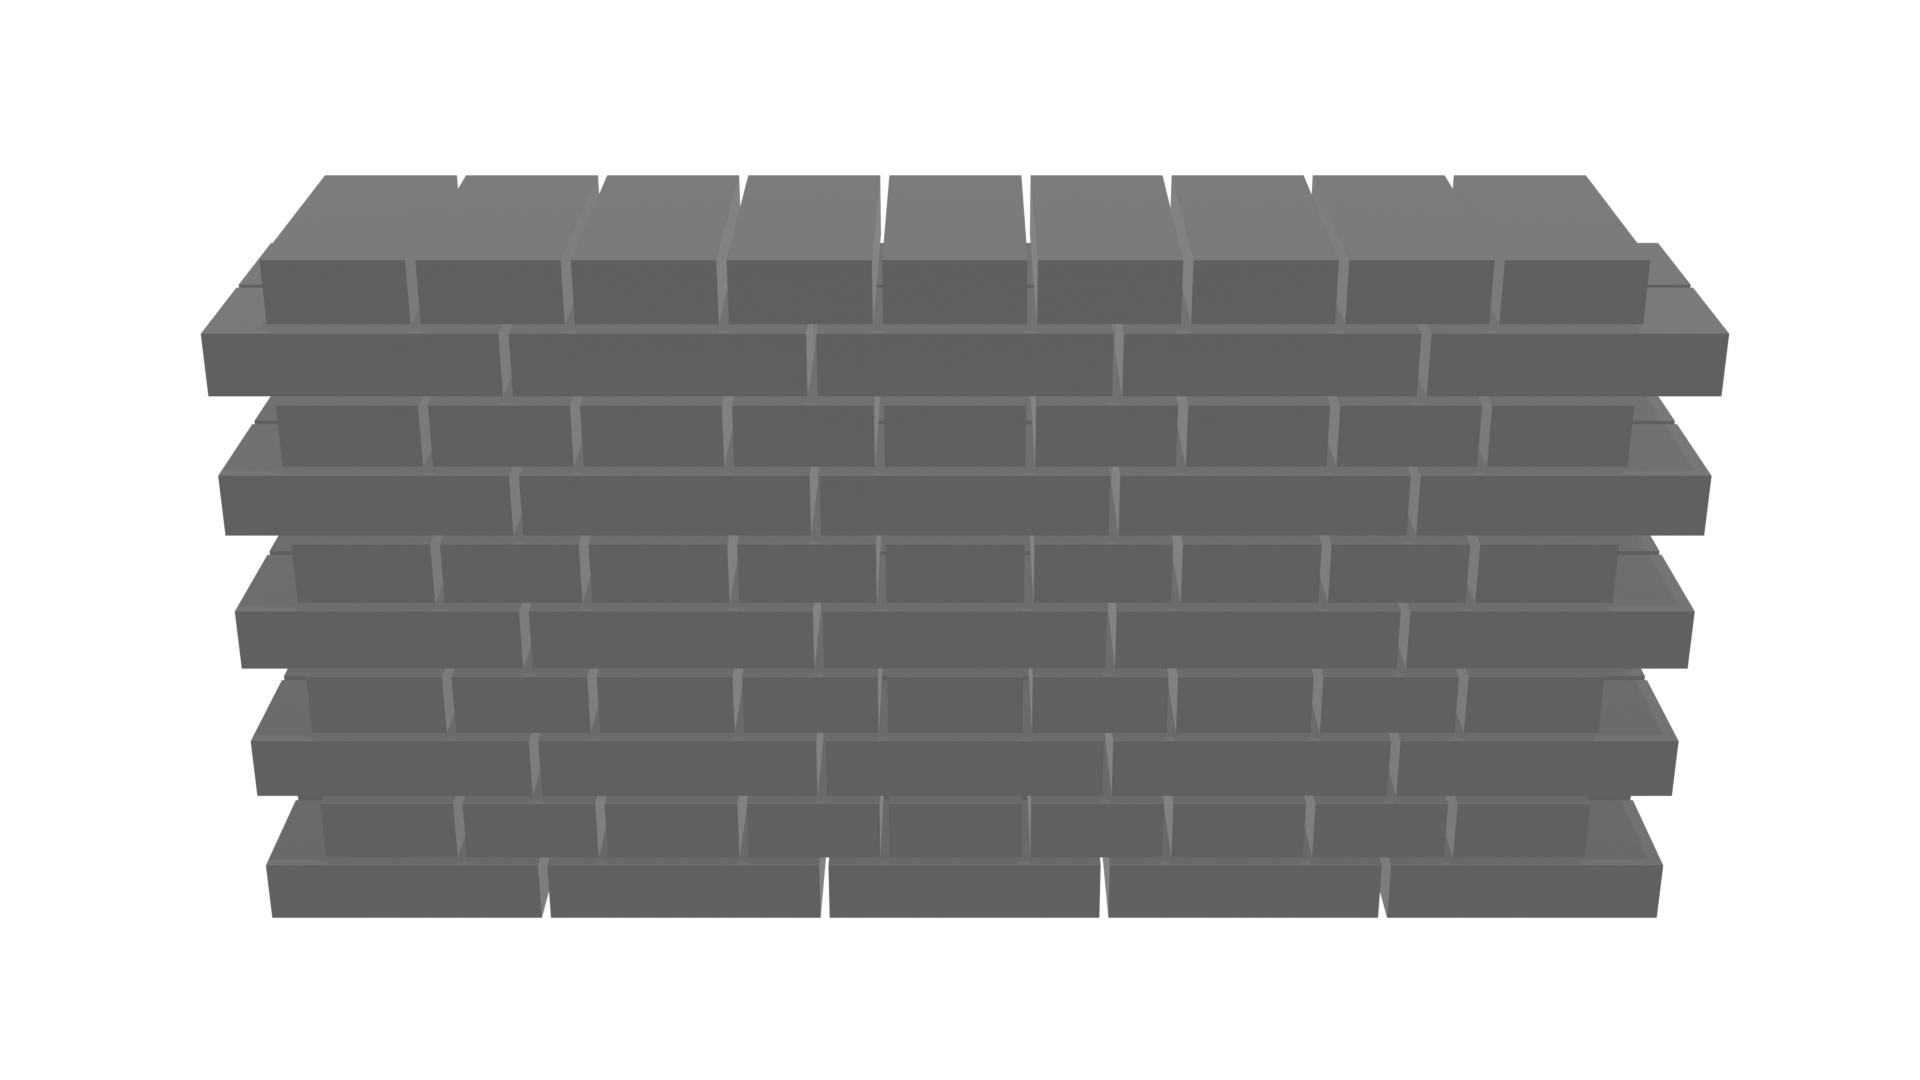
\includegraphics[width=\columnwidth]{fig/blockverband.png}
    \caption{Blockverband.}
    \label{fig:basics:blockverband}
  \end{subfigure}
  \hfill
  \begin{subfigure}[b]{0.5\columnwidth}
    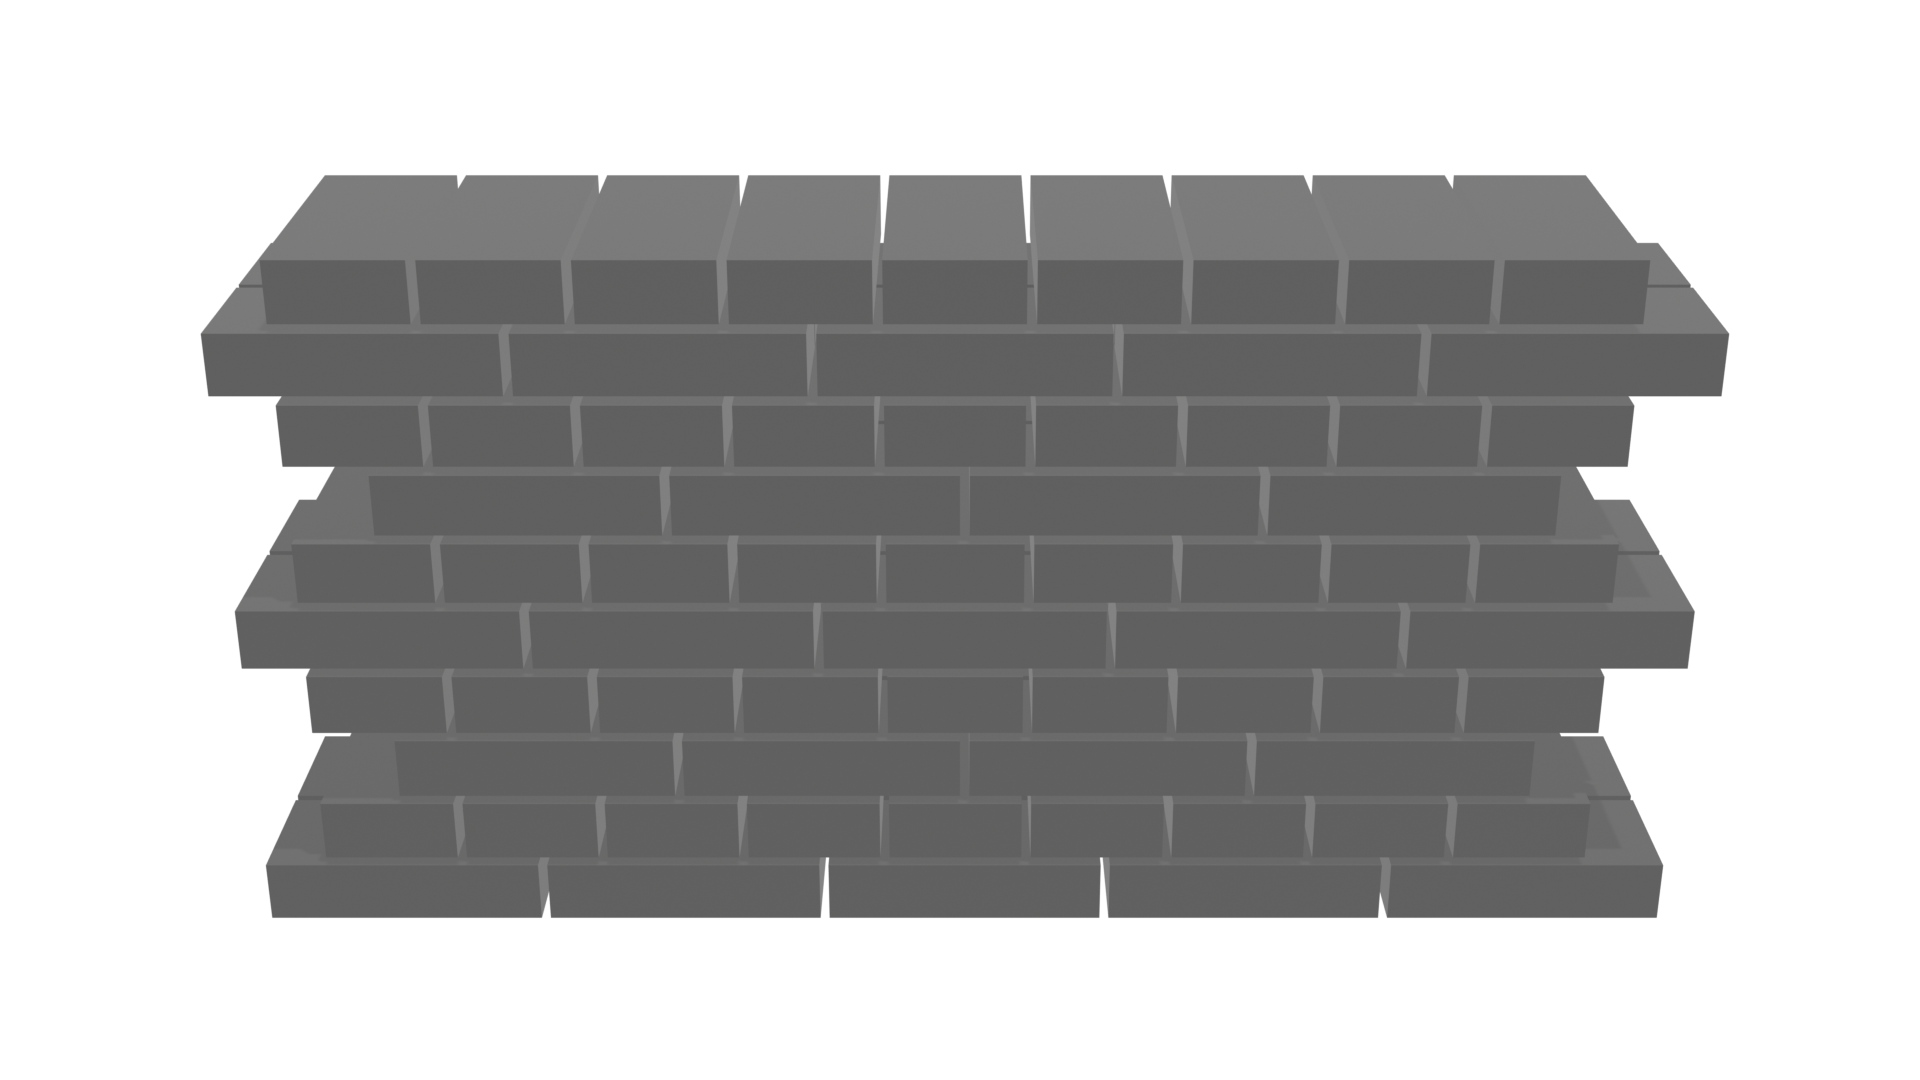
\includegraphics[width=\columnwidth]{fig/kreuzverband.png}
    \caption{Kreuzverband.}
    \label{fig:basics:kreuzverband}
  \end{subfigure}
  \begin{subfigure}[b]{0.5\columnwidth}
    \includegraphics[width=\columnwidth]{fig/läuferverband025_mittig.png}
    \caption{Mittlerer Läuferverband \textit{(1/4 Versatz).}}
    \label{fig:basics:laeuferverband_mittig}
  \end{subfigure}
  \begin{subfigure}[b]{0.5\columnwidth}
    \includegraphics[width=\columnwidth]{fig/läuferverband033_schleppend.png}
    \caption{Schleppender Läuferverband \textit{(1/3 Versatz).}}
    \label{fig:basics:laeuferverband_schleppend}
  \end{subfigure}
  \begin{subfigure}[b]{0.5\columnwidth}
    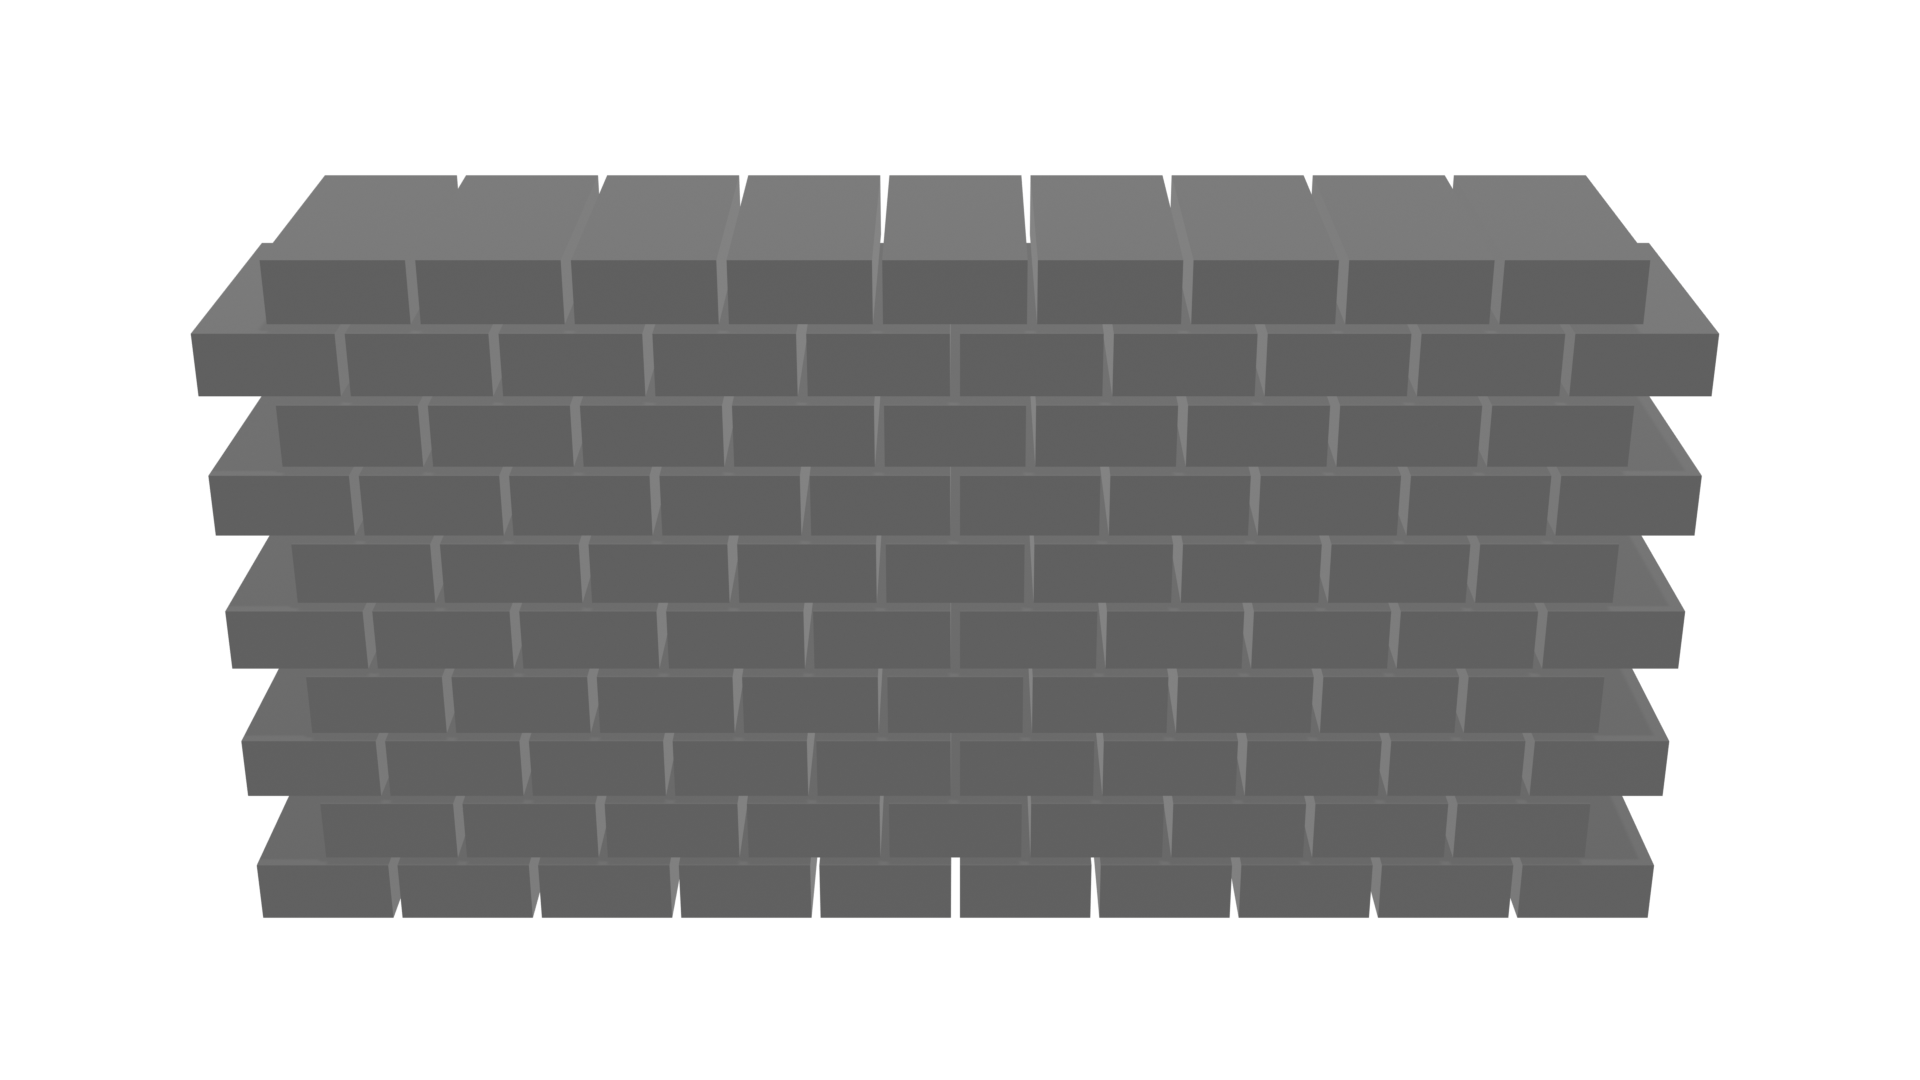
\includegraphics[width=\columnwidth]{fig/kopfverband.png}
    \caption{Kopf/Binderverband.}
    \label{fig:basics:binderverband}
  \end{subfigure}
  \begin{subfigure}[b]{0.5\columnwidth}
    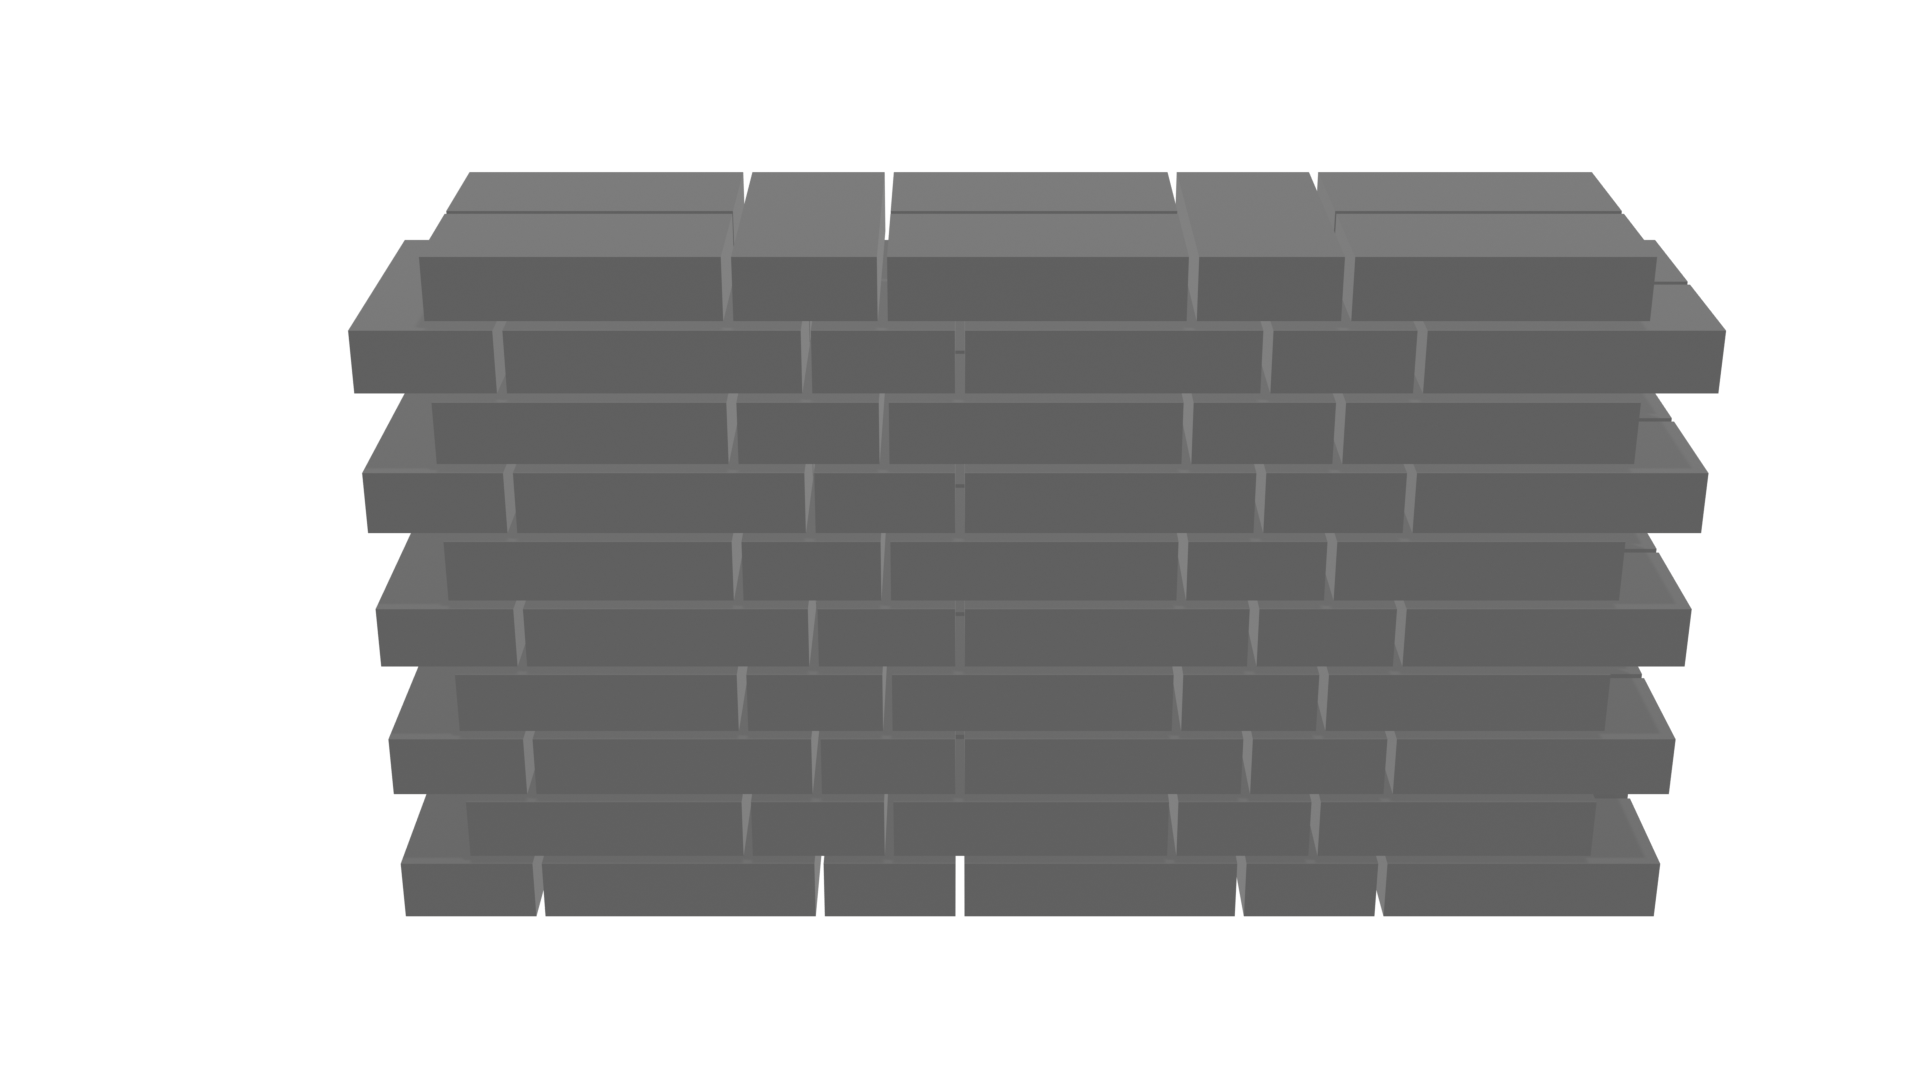
\includegraphics[width=\columnwidth]{fig/gotischerverband.png}
    \caption{Gotischer Verband.}
    \label{fig:basics:gotischer_verband}
  \end{subfigure}
  \caption{Typische Mauerwerksverbände.}
  \label{fig:basics:verbaende}
\end{figure}
Als Wandstück wird von nun an ein gerader Wandabschnitt bezeichnet.
Dieser hat eine Länge, eine Höhe und durch einen vorgegebenen Bausteintyp und einem gewünschten Verband eine gewisse Breite.
Treffen zwei oder mehrere Wandstücke aufeinander, so gilt es diese dem Überbindemaß entsprechend miteinander zu verzahnen.
Dabei treten verschiedene Sonderfälle auf, die für unterschiedliche Verbände nach unterschiedlichen Lösungen verlangen:
\begin{itemize}
  \item \textbf{Ecken} werden durch zwei sich an Wandenden berührenden, meist rechtwinklig zueinanderstehenden Wandstücken gebildet.
  \item \textbf{Kreuzungen} stellen zum Beispiel zwei sich kreuzende Wandstücke dar.
  \item \textbf{T-Kreuzungen} entstehen, wenn ein Wandende des einen Wandstücks auf einer anderen Wand steht.
  Sowohl bei Kreuzungen als auch T-Kreuzungen kann auf das aufwendige Verahnen verzichtet und stattdessen die sogenannte Stumpfstoßtechnik angewandt werden.
  Dabei werden Stahlanker zwischen der Wand und den darauf treffenden \glqq{}stumpfen\grqq{} Wandenden verwendet, um die beiden Wände sicher miteinander zu verbinden.
  \item \textbf{Wandenden} sind die \glqq{}Enden\grqq{} eines Wandstücks, die kein anderes Wandstück berühren.
  Dafür muss der verwendete Mauerwerksverband zu einem geraden Abschluss gebracht werden.
  Oftmals lässt sich das Anpassen der Bausteine (etwa durch zerschneiden) nicht vermeiden.
  \item \textbf{Öffnungen} innerhalb eines Wandstücks können in der selben Art behandelt werden, da der vorherrschende Verband in den betroffenen Schichten gerade unterbrochen werden muss.
  Über Öffnungen für Fenster und Türen wird ein sogenannter Sturz gelegt, welcher ebenfalls in den der Wand zugrunde liegenden Mauerwerksverband eingebunden werden muss.  
\end{itemize}
Die Lösungen für die oben geannten Situationen variieren je nach angestrebten Mauerwerksverband und der verwendeten Modulgröße stark.
Einige Beispiele sind in Abbildung~\ref{fig:basics:mauerwerk_eckloesung} und Abbildung~\ref{fig:basics:Kreuzungsloesung} zu sehen~\cite{Moro2021}\cite{MaurerfibelKreuzungen:online}.
Während etwa beim Läuferverband darauf verzichtet werden kann Bausteine für Eckbereiche und Kreuzungen zu zerschneiden, ist dies für andere Verbände teilweise unumgänglich. 

\begin{figure}[h]
  \centering
  \includegraphics[width=0.8\columnwidth]{fig/Eck- und Kreuzungslösungen.png}
  \caption{Lösungen für Ecken und T-Kreuzungen unterschiedlicher Verbände~\cite{Moro2021}}
  \label{fig:basics:mauerwerk_eckloesung}
\end{figure}

\begin{figure}[h]
  % https://www.ks-maurerfibel.de/maurerfibel/4-mauerwerksverbaende/4-7-mauern-von-stoessen-und-kreuzungen/ 
  \centering
  \includegraphics[width=0.8\columnwidth]{fig/KreuzungslösungBeispiel.png}
  \caption{Lösung einer Kreuzung am Beispiel einer \glqq{}Wand aus 2 DF im Kreuz- und Blockverband\grqq{}~\cite{MaurerfibelKreuzungen:online}}
  \label{fig:basics:Kreuzungsloesung}
\end{figure}

%https://baulexikon.beuth.de/MAUERWERKSVERBAND.HTM
%https://www.bauprofessor.de/mauerwerksverband/
%DIN 1053-1 (wurde durch DIN EN 1996-1-1 ersetzt)
%anstoßendes Wandstück: der bereich an dem zwei wandsegmente aneinanderstoßen z.b eine ecke
%https://www.baunetzwissen.de/mauerwerk/fachwissen/planungsgrundlagen/verbaende-und-verzahnung-162752
%Verzahnung: aus https://baulexikon.beuth.de/VERZAHNUNG.HTM : Verzahnung, im Mauerwerksbau übliche Technik, beim Herstellen einer Wand eine Verbindungsstelle für eine später zu errichtende und in die bereits bestehende einzubindende Wand den Verbandsregeln entsprechend vorzubereiten. Es gibt Lochverzah- nung, stehende und liegende Verzahnung. Nur die letztgenannte Verzahnungsart gilt nach DIN 1053-1 als ausreichende Verbindung zwischen tragenden und aussteifenden Mauerwerkswänden
%Überbindemaß ist wichtig um Mauerwerksverbände zu bewerten
%https://www.mauerwerksbau-lehre.de/vorlesungen/1-grundlagen-und-baustoffe-des-mauerwerksbaus/13-wandkonstruktionen/132-mauerwerksverband-und-ueberbindemass
%TODO Rund Wände, keine 90 Grad Ecken

\section{LEGO}
\label{basics:lego}
Ein 1$\times$1 LEGO Stein hat eine quadratische Grundfläche von \(7.8mm\)$\times$\(7.8mm\).
Dies entspricht demnach dem Baunennmaß des 1$\times$1 LEGO Steins.
Zwischen zwei nebeneinander platzierten Steinen ist ein Abstand von  \(0.2mm\).
Daraus ergibt sich ein Baurichtmaß beziehungsweise ein Rastermaß von \(8mm\)$\times$\(8mm\).
In Abbildung~\ref{fig:basics:Lego 2x4 Brick} werden zur Veranschaulichung die Maße des populären 2$\times$4 Steines aufgeschlüsselt.
Die für ein dreidimensionales Maß noch fehlende Größe ist die Höhe der Steine.
Diese beträgt \(9.6mm\).
Der Abstand zwischen zwei übereinander gestapelten Steinen hängt von dem Druck ab, der beim Zusammenstecken geleistet wurde.
Dennoch kann dieser vernachlässigt, sprich als Abstand von \(0.0mm\) gewertet werden.

\begin{figure}[h]
    \centering
    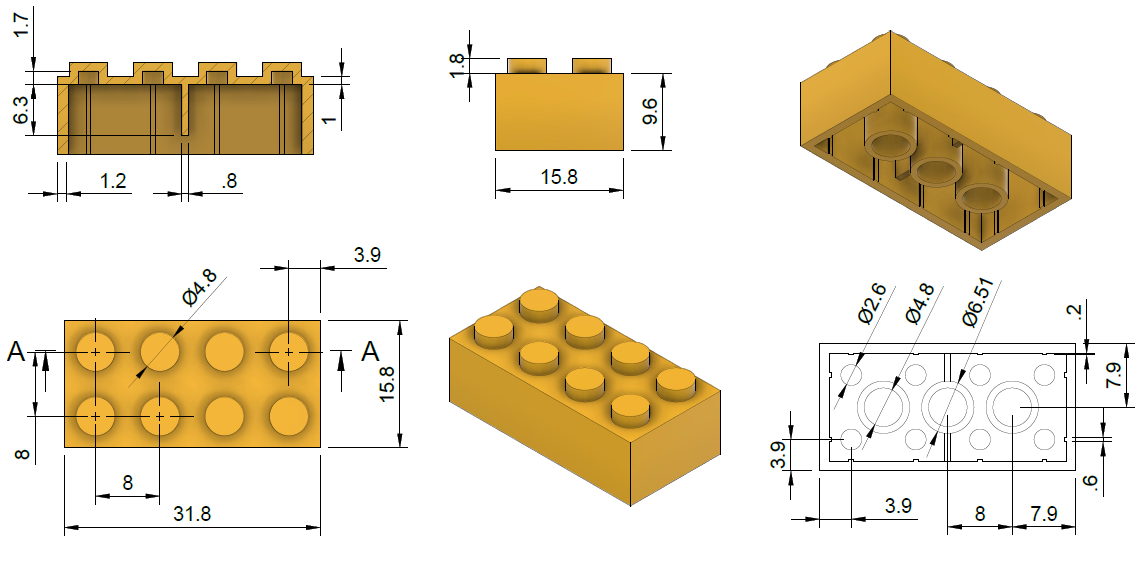
\includegraphics[width=0.8\columnwidth]{fig/LEGO 2x4 Brick horizontal.png}
    \caption{Maße des Standard 2$\times$4 LEGO Steins~\cite{LEGOBric2:online}}
    \label{fig:basics:Lego 2x4 Brick}
\end{figure}

\section{BRep}
\label{basics:brep}
Mal schauen

\section{Ontologie}
Der Begriff Ontologie stammt ursprünglich aus der Philosophie.
Wörtlich übersetzt bedeutet er \glqq{}Lehre des Seins\grqq{}.
Ein Definitionsvorschlag lautet wie folgt (aus dem Englischen):
\glqq{}Die Ontologie als Teilgebiet der Philosophie ist die Wissenschaft von dem, was existiert, den Arten und Strukturen von Objekten, Eigenschaften, Ereignissen, Prozessen und Relationen in allen Bereichen der Wirklichkeit\grqq{}~\cite{Ontology}.
Eine Anmerkung, die oftmals im Anschluss eines Definitionsvorschlags zu finden ist, besagt, dass dabei nicht nur das, \textit{was ist}, sondern ebenfalls das, \textit{was sein könnte} betrachtet werden müsse~\cite{Ontology}\cite{OntologieDefinitionLMU:online}.
Dieser Gedanke spiegelt sich ebenfalls in dem Ontologiebegriff aus der Informatik wider und ist unter dem Begriff \textit{Open World Assumption} bekannt.
Dies wird nach der Definition von Ontologien im Kontext der Informatik noch einmal ausführlicher aufgegriffen.

Im Fachbereich der Informatik wurde der Begriff Ontologie adaptiert und zunächst als \glqq{}explicit specification of a conceptualization\grqq{} definiert~\cite{Gruber1993}.
Wörtlich übersetzt lautet diese Definition etwa \glqq{}explizite Spezifizierung einer Konzeptualisierung\grqq{}.
Im Laufe der Jahre wandelte sich diese Definition, sodass sich daraus zum Beispiel folgendes ergab: \glqq{}An ontology is a formal, explicit specification of a shared conceptualization\grqq{}~\cite{Studer1998}.
Hier wird eine Ontologie also als \glqq{}formale, explizite Spezifizierung einer geteilten Konzeptualisierung\grqq{} bezeichnet.
Den wichtigsten Zusatz hierbei stellt das Wort \glqq{}geteilt\grqq{} dar, da Ontologien unter anderem dem Zweck dienen, Informationen und Vokabulare mehrerer Wissensrepräsentation zu vereinen.
Der Begriff Konzeptualisierung wird oft als \glqq{}vereinfachte, abstrakte Sicht auf einen für einen bestimmten Nutzen relevanten Teil der Welt\grqq{} beschrieben~\cite{Guarino2009}.

Eine solche \glqq{}Spezifizierung einer Konzeptualisierung\grqq{} einer gewissen Domäne kann heutzutage mithilfe der sogenannten \textit{Web Ontology Language} (OWL), welche auf dem \textit{Resource Description Framework} (RDF) aufbaut, realisiert werden~\cite{OWL_W3C}\cite{RDF_W3C}.
OWL erlaubt es Klassen zu definieren und daran Eigenschaften anzuheften.
Außerdem können sogennante Individuen beziehungsweise Instanzen erstellt werden.
Diese realisieren eine oder mehrere Klassen.
Mithilfe dieser Klassen, Eigenschaften und Individuen können sogennante \textit{Reasoner} logische Schlussfolgerungen über implizit angegebenes Wissen ziehen.
Eine Ontologie kann damit einerseits etwa mit neuen Klassenzuordnungen oder implizit angegeben Vererbungen erweitert, andererseits auf Validität überprüft werden.
Werden Verletzungen von aufgestellten Axiomem oder widersprüchliche Einschränkungen von Klassen oder Eigenschaften entdeckt, so kann ein Reasoner diese nicht nur melden, sondern auch mithilfe logischer Beweisführung herleiten.
Damit stellen Reasoner ein wertvolles Werkzeug für die Entwicklung und Erweiterung von Ontologien dar.
Drei weit verbreitete Reasoner sind: 
\begin{itemize}
  \item ELK Reasoner der Universitäten Ulm und Oxford~\cite{Kazakov2014}.
  \item HermiT Reasoner von der \textit{Information Systems Group} der Universität Oxford~\cite{Glimm2014}\cite{HermitReasoner:online}.
  \item Open Source Pellet Reasoner der Clark \& Parsia LLC~\cite{Sirin2007}. 
\end{itemize}
Aufgrund der oben genannten Idee der \textit{Open World Assumption} unterscheidet sich die Art der Reasoner logische Schlussfolgerungen zu ziehen von der, mit welcher logische Aussagen von zum Beispiel Programmiersprachen bewertet werden.
Im Grunde versteht man unter der \textit{Open World Assumption}, das nicht Falsifizieren eines logischen Ausdrucks, falls Wissen exisitieren könnte, das den Ausdruck doch verifizieren würde.
Ein Reasoner beziehungsweise eine Programmiersprache im Kontext der \textit{Closed World Assumption} würde in so einer Situation davon ausgehen alle exisitierenden Informationen darüber bereits vorliegen zu haben und eventuell zu einem anderen Schluss gelangen.
Definiert man zum Beispiel eine Klasse A als alle Individuen, die nur eine Eigenschaft E besitzen, die sie mit Individuen einer bestimmten anderen Klasse B verbindet, so kann ein Reasoner innerhalb dieser Ontologie ein Individuum, das zwar diese Anforderung erfüllt, nicht der Klasse A zuordnen, da es sein kann, dass zu einem späteren Zeitpunkt (oder an anderer Stelle) Informationen existieren, die diese Zuordnung fehlerhaft machen würden.
In einer Umgebung, in der die \textit{Closed World Assumption} gilt, wäre diese Zuordnung hingegen völlig korrekt.
Deren Annahme einer \textit{offenen Welt} ermöglicht es ebenfalls die Idee des sogenannten \glqq{}Semantic Web\grqq{} mithilfe von Ontologien zu realisieren~\cite{SemanticWebLee}.
Denn die Natur des Internets entspricht eher einer sich ständig ändernden und \glqq{}offenen\grqq{} Welt, als einer Geschlossenen.
Als Semantic Web wird das Annotieren von sämtlichen Webinhalten mit semantischen Informationen bezeichnet.
Damit wird das Ziel verfolgt, ein maschinenlesbares Internet zu schaffen. 
%TODO: da nochmal genauer drauf eingehen und semantic web kurz erwähnen -> wissen könnte ja noch iwo im internet sein, außer explizit anders angegeben.

\subsection{Protégé}
Protégé ist ein graphischer Editor zur Erstellung und Instandhaltung von Ontologien~\cite{Protege}.
Entwickelt wird das Programm an der Universität Stanford und ist als Open Source Anwendung kostenfrei nutzbar.
Die erste Version wurde bereits 1999 veröffentlicht.
Durch seine Plugin-Struktur können neben zahlreichen Erweiterungen beispielsweise auch neue Reasoner an das Programm angeschlossen werden.
Standardmäßig sind der ELK und der HermiT Reasoner integriert, aber es exisitieren Plugins um auch Pellet in Protégé zu nutzen.
Das Arbeiten mit einem graphischen Editor erleichtert den Einstieg in das Thema und ermöglicht später einen besseren Überblick über oftmals umfangreiche Ontologien, als es in einem herkömmlichen Texteditor möglich wäre.
Darum wurde das Programm zur Erstellung einer Ontologie für diese Arbeit herangezogen.

\subsection{Owlready2}
Owlready2 ist eine Python 3 Bibliothek, die es ermöglicht \glqq{}ontologie-orientiert\grqq{} zu programmieren~\cite{Owlready}.
Bisher mussten Ontologien mithilfe von Abfragesprachen (etwa SPARQL) oder APIs bearbeitet und ausgewertet werden~\cite{SPARQLF_W3C}.
Owlready2 bietet hingegen einen einfacheren Umgang mit Ontologien, ebnet damit den Einstieg in das Thema und ermöglicht gleichzeitig die Integration von Ontologien in jedes mit Python umsetzbare Projekt.
Im Zusammenspiel mit Protégé bietet diese Bibliothek eine für Programmierer intiuitive Möglichkeit, die oben genannten Werkzeuge für IFC und BIM durch Nutzung von Python 3 direkt mit der Technologie der Ontologien zu koppeln.

\chapter{Konzept}
Dieser Einleitungssatz leitet mit durchdachten Worten das Kapitel ein, in dem es um die Konzepte geht, die ich mir ganz sicher vor der Implementierung ausgedacht habe!
Hier ist allerdings anzumerken, dass dies nur ein Platzhalter ist und mithilfe dieses TODOs als solcher gekennzeichnet ist.
Ab jetzt sind wir aber alle mal wieder seriös.

\section{Modellierung}
Für gewöhnlich sind beim Planungsprozess eines Gebäudes oder anderer Infrastruktur eine Vielzahl an Experten aus unterschiedlichen Disziplinen beteiligt.
Ein Ziel dieser Arbeit ist es allerdings eine intuitive Konstruktionsplanung zu ermöglichen, sodass eine Einzelperson mit relativ geringer Einlern- und Modellierungszeit in der Lage ist ein Gebäude zu entwerfen.
Dieser Entwurf muss dennoch alle notwendigen Informationen für die anschließende Bauplandeduktion enthalten, ohne dass das Einpflegen dieser Daten spezielles Fachwissen voraussetzt.

Oftmals lässt sich die Komplexität einer Sache oder eines Vorgehens durch die Vorgabe von Einschränkungen reduzieren.
Dabei ist es allerdings wichtig diese Einschränkungen so zu wählen, dass die damit erzielten Ergebnisse nach wie vor von Nutzen sind.

\subsection{Raster}\label{concept:raster}
Im Fall von Gebäude- oder besser Gebilde-Konstruktionen existieren bereits einige Beispiele, die durch Einschränkungen so stark vereinfacht werden, dass sogar Kinder damit umgehen können.
Das wohl bekannteste ist das Lego System (siehe Kapitel~\ref{basics:lego}).
Neben dessen nützlichen Steckverbindungen, die es ermöglichen ohne Anwenden von Klebstoff oder Schrauben Steine aneinander zu befestigen, ist für diese Arbeit das dadurch vorgegebene Raster ein interessantes Konzept zur Vereinfachung der Modellierung von Gebäuden.
In Kapitel~\ref{basics: Mauerwerksbau} wurden auch schon die Begriffe \textit{Baunennmaß} und des \textit{Baurichtmaß} eingeführt und das oktametrischen Maßsystem vorgestellt.
Dies entspricht im Prinzip ebenfalls einem Raster, das aber in Realität durch die Möglichkeit des Zerschneidens von Bausteinen nicht zwingend eingehalten werden muss.
Da das Vorgeben eines Rasters, dem sowohl die Größen der zu verwendenden Bausteine, als auch (im Fall des Lego Systems) deren Platzierung folgen müssen, eine Einschränkung darstellt, die im Einklang mit der Intuition vieler Menschen steht, wurde dies in das Modellierungskonzept dieser Arbeit integriert.
Das Vorgeben eines einzigen, fest definierten Rasters stellt allerdings eine zu große Einschränkung dar, weshalb das Definieren verschiedener Rastergrößen möglich sein muss.
So können Modelle erstellt werden, die sowohl genau dem Lego System oder dem oktametrischen Maßsystem entsprechen, als auch beliebig anderen Rastern.

Die Modellierungsumgebung kann mithilfe von Rasterinformationen eines Objektes für dessen korrekte Platzierung, Skalierung und Rotierung sorgen, indem eine solche Transformation auf die nächstliegende Größenordnung des Rasters gerundet wird.
Im Beispiel eines Rasters von \([1.0m, 1.0m, 1.0m]\) würde demnach ein auf \([0.9m, -0.7m, 0.1m]\) zu translatierendes Objekt an die Position \([1.0m, -1.0m, 0.0m]\) versetzt werden.
Da aber gewünschte valide Rotationen nicht aus einem derart vorgegebenen Raster interpretierbar sind, kann diese zusätzliche Information mithilfe eines kleinstmöglichen Winkelschritts angegeben werden.
In den Modellen der Fallstudien aus Kapitel~\ref{scenarios} werden zum Beispiel ausschließlich Rotationen eines Vielfachen von 90\degree{} verwendet, was neben den Rastern ebenfalls hinterlegt wurde.
Damit kann die Modellierungsumgebung auch den Rotationen von Objekten durch Runden eine Art Raster aufzwingen.

\subsection{Wandstück}
Auch die schiere Menge verschiedener Bestandteile eines Hause ist für eine Einzelperson ohne Vorkenntnisse nicht überblickbar.
Da das Ziel dieser Arbeit das automatische Generieren von Legeplänen für Bausteine innerhalb der Wände eines Gebäudes darstellt, lässt sich diese Menge vorerst auf zwei wesentliche Objekttypen reduzieren:
Wände und Öffnungen in Wänden.
Öffnungen werden zum Beispiel für Fenster oder Türen benötigt.
Da eine Wand im Prinzip ein arbiträrer geometrischer Körper sein kann, dies abzubilden aber wieder die Komplexität der Modellierung steigert, wird deren Form auf einen beliebig skalierten Quader beschränkt.
Ein solcher Quader wird nachfolgend auch als \textit{Wandstück} bezeichnet.
Ein solches Wandstück besitzt demnach auch die Eigenschaften eines Quaders: eine Skalierung, eine Rotation um seinen eigenen Mittelpunkt und eine Translation im Raum.
Nachfolgend werden die Begriffe Länge, Breite und Höhe zur einfachen Unterscheidung von einer Skalierung in X, Y und Z Richtung verwendet.
Während Länge und Höhe dem Raster entsprechend beliebig gewählt werden können, ergibt sich die Breite aus dem gewählten Bausteinformat (auch als \textit{Modul} bezeichnet) und dem geplanten Mauerwerksverband (siehe Kapitel~\ref{basics:mauerwerk}).
Der Verband und das Modul können jedem Wandstück als sogenannter \textit{Wandtyp} zugewiesen werden.
Dadurch ist es möglich, verschiedene Arten von Wänden innerhalb eines Gebäudemodells zu verwenden.
Diese Informationen werden später dafür verwendet, die durch das Wandstück abgesteckten Dimensionen sinnvoll mit Bausteinen zu füllen.

\subsection{Mauerwerksverband}\label{concept:mauerwerksverband}
In Kapitel~\ref{basics:Mauerwerksverband} wurden bereits einige verschiedene Mauerwerksverbände behandelt.
Um dem Wall Detailing Verfahren diese und beliebig andere Verbände in einer interpretierbaren Weise zur Verfügung stellen zu können, wird dafür eine mathematische Notation benötigt.
Bei genauer Betrachtung handelt es sich bei den meisten Mauerwerksverbänden um ein sich wiederholendes Muster.
Dabei wiederholen sich sowohl die Bausteintransformationen innerhalb einer Schicht des Verbandes, als auch dessen Schichten selbst.
Daher sind folgende Informationen zur Beschreibung eines Mauerwerksverbands notwendig:

\begin{enumerate}
    \item eine Menge einzigartiger Schichten, bis diese sich (mit einem Versatz) wiederholen.
    \item Für jede Schicht eine Menge verschiedener Bausteintransformationen, bis diese sich (ebenfalls mit einem Versatz) wiederholen.
\end{enumerate}

Ein Mauerwerksverband kann damit als Menge von Schichten verstanden werden, die sich wiederum aus einer Menge von Bausteintransformationen zusammensetzen.
Diese Schichten besitzen jeweils einen festgelegten, darunter liegenden Vorgänger sowie einen darüber liegenden Nachfolger.
Das bedeutet, die Reihenfolge in der Schichten eines Mauerwerksverbands auftreten, darf nicht verändert werden.
Leicht zu sehen ist dies am Beispiel eines Kreuzverbandes, der durch Veränderung der Reihenfolge seiner Schichten, seine typische kreuzartige Form verlieren würde.

Eine Bausteintransformationen wird in dieser Arbeit als Tupel mit folgendem Inhalt definiert:

\begin{enumerate}
    \item Eine skalierbare Position \(\vec{p} = {[x, y, z]}^T\).
    \item Eine skalierbare Rotation \(r = (x, y, z)\) angegeben in Euler-Winkeln.
    \item Einen festen translativen Versatz \(\vec{p}_o = {[x, y, z]}^T\).
    \item Einen festen rotierenden Versatz \(r_o = (x, y, z)\) ebenfalls in Euler-Winkeln.
\end{enumerate}

Skalierbar bedeutet in diesem Fall, dass die Werte von beispielsweise der Position eines Bausteins in Abhängigkeit eines veränderbaren Faktors stehen.
Zur endgültigen Platzierung eines Bausteins anhand einer Bausteintransformation aus einer Schicht eines Mauerwerksverbands wird lediglich noch ein Faktor benötigt, der angibt, die wievielte Wiederholung der Menge an Bausteintransformationen einer Schicht gerade Anwendung findet.
Sei \(B_1 = (\vec{p}, r, \vec{p}_o, r_o) = ({[l, 0, 0]}^T, (0, 0, 0), {[0, 0, 0]}^T, (0, 0, 0))\) eine Bausteintransformationen, \(M = (l, b, h) = (2, 1, 1)\) ein Modul und \(c\in\mathbb{N}\) ein Skalar,
dann ergibt sich die Position \(P\) eines Bausteins zur Wiederholung \(c = 1\) wie folgt: \(P = \vec{p}_o + c * \vec{p} = {[0, 0, 0]}^T + 1 * {[2, 0, 0]}^T = {[2, 0, 0]}^T\).
Im nächsten Wiederholungsschritt mit \(c = 2\) ergibt dies eine Position \(P = {[4, 0, 0]}^T\).
Da die Rotationen als Euler-Winkel vorliegen, kann diese in ähnlicher Weise berechnet werden.
Sie beschreibt die Rotation um den Mittelpunkt des Bausteins.
In den meisten Fällen ist \(r\) allerdings gleich \((0, 0, 0)\) und \(r_o\) entweder ebenfalls \((0, 0, 0)\) oder \((0, 0, \frac{\pi}{2})\).
Letzteres entspricht einer festen Rotation um 90\degree{} um die Z-Achse des Bausteins, unabhängig des Wiederholungsschritts \(r\).

\begin{figure}[hb!]
    \centering
    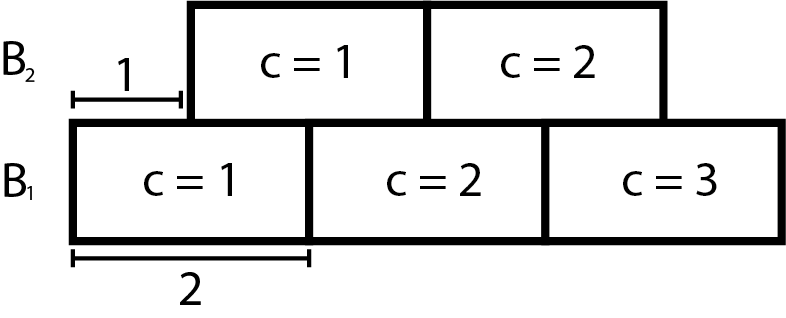
\includegraphics[width=0.7\columnwidth]{fig/concept_Mauerwerksverband.png}
    \caption{Der Läuferverband mit einem Versatz von 50\%.}
    \label{fig:concept:concept_Mauerwerksverband}
\end{figure}

Mit \(B_2 = ({[l, 0, 0]}^T, (0, 0, 0), {[\frac{l}{2}, 0, 0]}^T, (0, 0, 0))\) und je einer Schicht gebildet aus den Mengen \(\{B_1\}\) bzw. \(\{B_2\}\) erhält man bereits eine komplette Beschreibung für den Läuferverband mit einem Versatz von 50\% der Steinlänge.
Dieses Beispiel ist in Abbildung~\ref{fig:concept:concept_Mauerwerksverband} schematisch dargestellt.
Aber auch andere, komplexere Verbände können in dieser Form abgebildet und so dem nachfolgenden Wall Detailing in abstrahierter Weise übergeben werden.

\begin{figure}[ht!]
    \centering
    \begin{subfigure}[b]{0.3\columnwidth}
      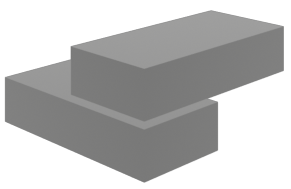
\includegraphics[width=\columnwidth]{fig/concept_streched_bond_corner.png}
      \caption{Erst \(E_1\), dann \(E_2\).}
      \label{fig:concept:concept_streched_bond_corner}
    \end{subfigure}
    \hfil
    \begin{subfigure}[b]{0.3\columnwidth}
      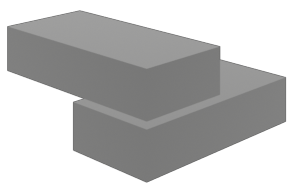
\includegraphics[width=\columnwidth]{fig/concept_streched_bond_corner_inverse.png}
      \caption{Erst \(E_2\), dann \(E_1\).}
      \label{fig:concept:concept_streched_bond_corner_inverse}
    \end{subfigure}
    \hfil
  \caption{Eckpläne für den Läuferverband mit einem Versatz von 50\%.}
  \label{fig:concept:corner_bond}
\end{figure}

Die speziellen Legepläne zur korrekten Auflösung von kritischen Bereichen wie zum Beispiel Ecken können ebenfalls in dieser Form für jeden Mauerwerksverband angegeben werden.
Für das vorangegangene Beispiel sähe der Eckplan wie folgt aus:
Eine Nulltransformation \(E_1 = ({[0, 0, 0]}^T, (0, 0, 0), {[0, 0, 0]}^T, (0, 0, 0))\) in der ersten Schicht und eine Bausteintransformationen 
\(E_2 = ({[0, 0, 0]}^T, (0, 0, 0), {[0, 0, 0]}^T, (0, 0, \frac{\pi}{2}))\) mit einer festen 90\degree{} Rotation um die Z-Achse in der Zweiten.
Dieser Eckplan ist in Abbildung~\ref{fig:concept:corner_bond} zu sehen.
Ein Beispiel, in welchem dieser Eckplan angewandt wird, wurde bereits in Abbildung~\ref{fig:basics:mauerwerk_eckloesung} in Kapitel~\ref{basics:Mauerwerksverband} gezeigt.
Der einzige Unterschied zwischen dem Plan eines Mauerwerksverbands für gerade Wände und dessen Spezialplänen ist deren Anwendung.
Während aus dem Eckplan später für jede Schicht nur ein Baustein pro hinterlegter Bausteintransformation erzeugt werden muss, können beliebig lange gerade Wandabschnitte mithilfe des oben angesprochenen Wiederholungsschritts mit Bausteinen aufgefüllt werden.

\subsection{Beziehungen zwischen Wandstücken}\label{concept:relations_wandtuecke}
In dieser Arbeit stehen Wandstücke zueinander in einer Beziehung, sobald sie sich berühren oder schneiden.
Diese Beziehungen sind relevant, um die gewählten Mauerwerksverbände ordnungsgemäß über mehrere voneinander abhängige Wandstücke anzuwenden, ohne dass es zu Verletzungen von Vorschriften und Normen wie etwa dem Überbindemaß aus Kapitel~\ref{basics:Mauerwerksverband} kommt.
Wie bereits in Abschnitt~\ref{scenarios:scenario1:problem} und~\ref{basics:Mauerwerksverband} angesprochen, treten verschiedene Arten von Beziehungen auf, die für das nachfolgende \glqq{}Wall Detailing\grqq{} zu unterscheiden sind.
Zur Modellierung von Gebäuden sind vor allem folgende Beziehungen unabdingbar:
\textit{Ecken}, \textit{T-Kreuzungen} und \textit{X-Kreuzungen}.
Diese stellen wichtige Elemente bei der Planung von Gebäuden dar. 
Nur so ist es möglich abgeschlossene und aneinanderhängende Räume zu erstellen.
Eine weitere, nicht ganz offensichtliche Beziehung besteht zwischen zwei Wandstücken, die in Verlängerung zueinander stehen, also gemeinsam einen größeren Wandbereich abdecken.
Diese Beziehung wird nachfolgend \textit{Wandstückverbund} genannt.
Bei allen vier Beziehungen handelt es sich Sonderfällle, für welche sich der Mauerwerksverband nicht ohne weiteres anwenden lässt, sondern teilweise explizit vorgegebene Legepläne angewandt werden müssen.
Darum ist es notwendig diese Bereiche ausfindig zu machen und voneinander unterscheiden zu können.
Es werden nun für jede dieser Beziehungen Eigenschaften aufgezeigt anhand derer man diese in einer Menge an Wandstücken erkennen kann.

\begin{figure}[ht]
    \centering
    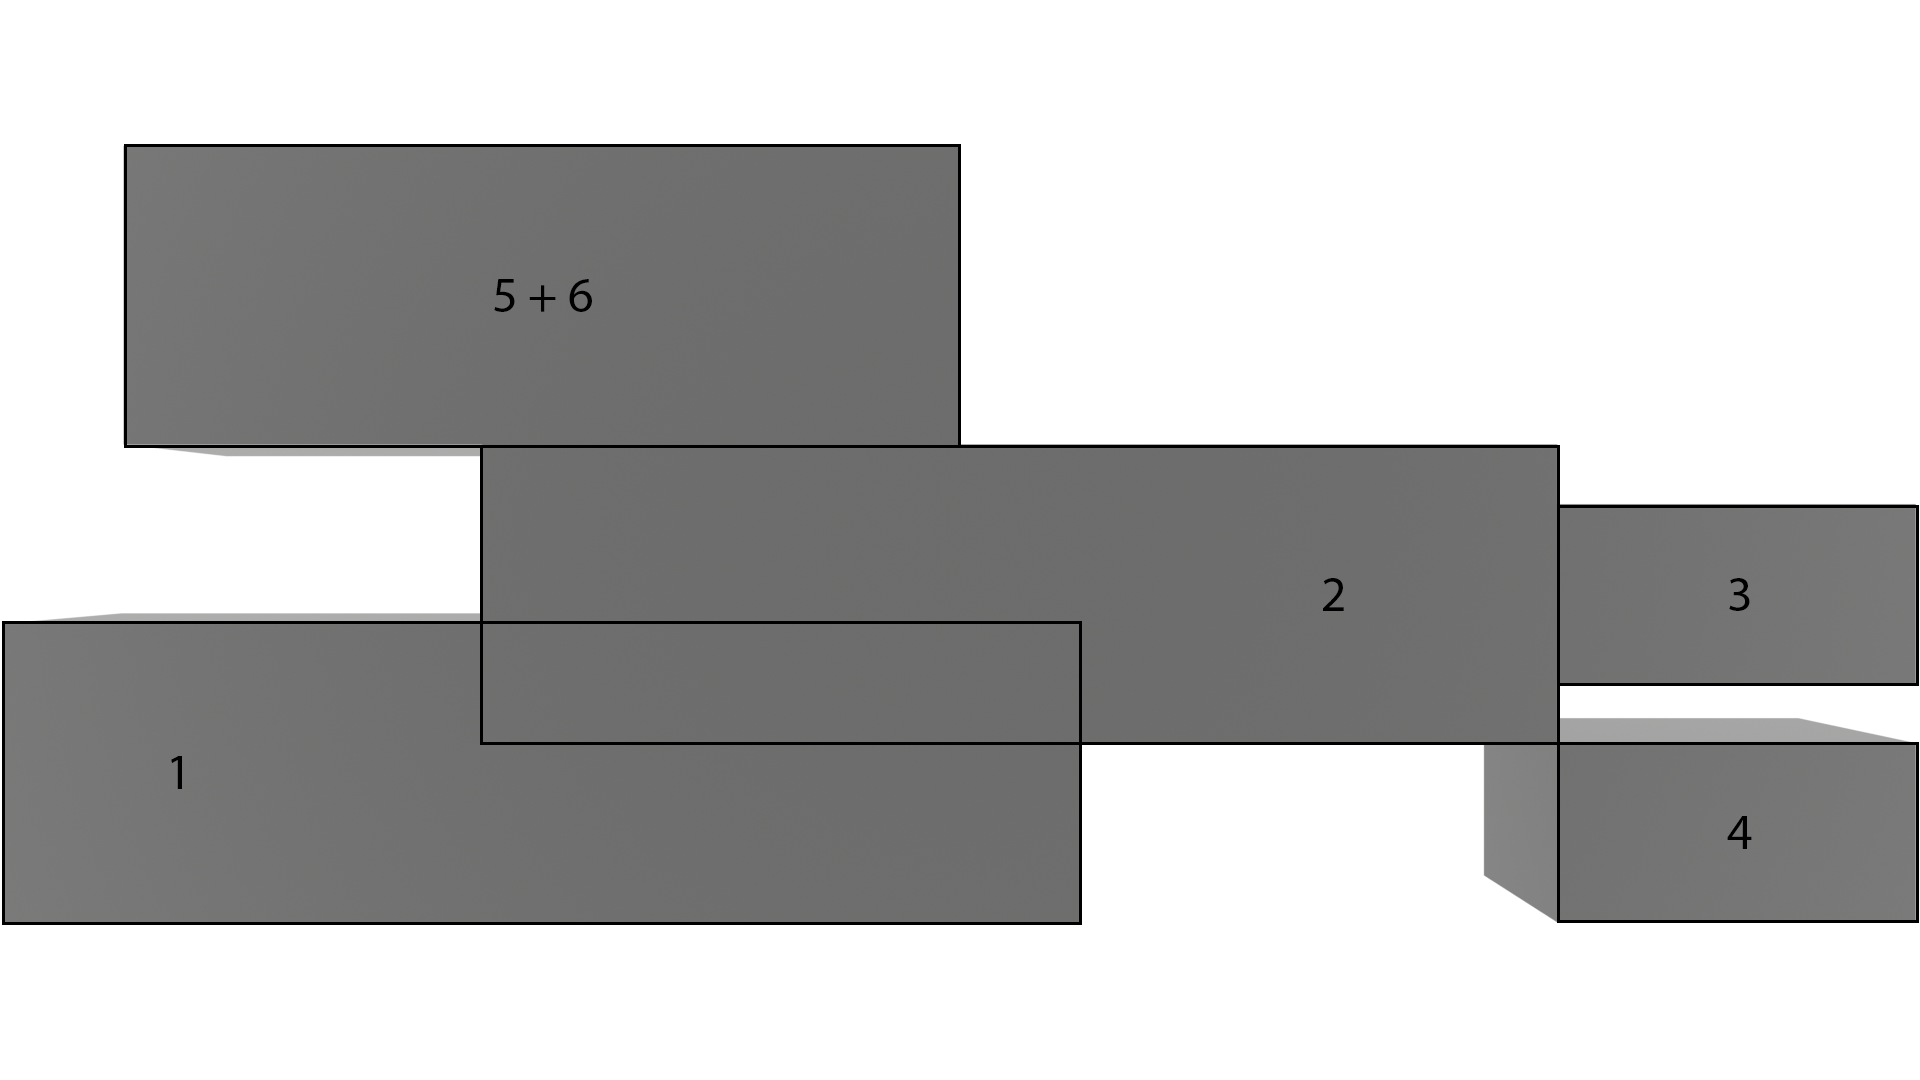
\includegraphics[width=0.8\columnwidth]{fig/Real_Combination_Base_labeled.png}
    \caption{Modell einer Wand, die durch 7 einzelne Wandstücke des selben Typs gebildet wird, deren Mittelpunkte alle auf einer Ebene liegen.}
    \label{fig:concept:combination_example_base}
\end{figure}

\paragraph*{Wandstückverbände}\label{concept:combination_properties} sind alle Wandstücke,  die zwar in dem Modellierungsprozess des Gebäudes durch mehrere einzelne Wandstücke realisiert wurden, eigentlich aber eine Einheit darstellen. 
Es ist notwendig alle Wandstücke zu identifizieren, die einen zusammenhängenden Wandbereich bilden, um den gewählten Mauerwerksverband korrekt über alle Wandstücke hinweg anzuwenden.
Andernfalls würde jedes Wandstück den Mauerwerksverband unabhängig seiner Nachbarn neu beginnen und ihn dadurch zwischen Wandstückübergängen häufig fälschlicherweise unterbrechen.
Ein umfangreiches Beispiel ist in Abbildung~\ref*{fig:concept:combination_example_base} dargestellt.
Um zu überprüfen, ob zwei Wandstücke eine Einheit bilden, kann das Paar auf folgende Eigenschaften getestet werden:

\begin{enumerate}
    \item Beide Wandstücke verwenden das selbe Modul und sind während der Modellierung mit den gleichen Wandtyp annotiert worden. 
    Dies verhindert vor allem das Kombinieren unterschiedlich dicker Wände.
    \item\label{real:z_parallel} Die lokalen Z-Achsen beider Wandstücke sind parallel. 
    Dies verhindert das Kombinieren unpassend rotierter Wandstücke.
    Die Überprüfung der Parallelität der Z-Achsen beider Wandstücke wird wie folgt durchgeführt:

    Sei \(\vec{v}_z = {[0, 0, 1]}^T\)
    eine Z-Achse und \(v_z = (v_w, v_x, v_y, v_z) = (0, 0, 0, 1)\) das dazugehörige Quaternion. 
    Außerdem seien \(q_1\) und \(q_2\) die beiden Rotationen der Wandstücke. Dann stellen 
    \(v_{z^1} = q_1 * v_z * q_1^{-1}\) und 
    \(v_{z^2} = q_2 * v_z * q_2^{-1}\) die jeweiligen \glqq{}Z-Anteile\grqq{} dieser Rotationen dar.
    Daraus ergeben sich die \glqq{}Z-Vektoren\grqq{} wie folgt: 
    \(\vec{v}_{z^1} = {[v_{z^1_x}, v_{z^1_y}, v_{z^1_z}]}^T\) und
    \(\vec{v}_{z^2} = {[v_{z^2_x}, v_{z^2_y}, v_{z^2_z}]}^T\).
    Ist nun \(|\vec{v}_{z^1} \cdot \vec{v}_{z^2}| = 1\) gegeben, so sind die lokalen Z-Achsen der Wandstücke gleich oder um exakt 180\degree{} verdreht und damit Parallelität erfüllt.
    \item Die lokalen X-Achsen beider Wandstücke sind ebenfalls parallel. Das Vorgehen zur Überprüfung entspricht dem von Punkt~\ref{real:z_parallel}, nur dass \(v_z\) durch \(v_x = (0, 1, 0, 0)\), also der X-Achse, ersetzt werden muss.
    \item Sie stehen auf der selben Höhe oder versetzt um ein Vielfaches der gemeinsamen Modulhöhe.
    \item\label{concept:schichten} Es liegt eine Berührung oder gar eine Überlappung vor.
\end{enumerate}

Insgesamt bilden in dem Beispiel in Abbildung~\ref{fig:concept:combination_example_base} demnach alle Wandstücke mit Ausnahme von Wandstück Nummer 4 eine Einheit, die alle obigen Eigenschaften erfüllt.
Dies sind in der Tat all die Wandstücke, die den Start des gewählten Mauerwerksverbands ihren Nachbarn entsprechend anpassen müssen, sodass sich der Verband gleichmäßig über alle Wandstücke erstreckt.

\paragraph*{Ecken, T-Kreuzungen und X-Kreuzungen}\label{concept:corner_etc_properties} stellen Beziehungen zwischen einzelnen Wandstücken oder den kombinierten Wandstückverbänden aus Abschnitt~\ref{concept:combination_properties} dar.
Wie schon zu Beginn dieses Abschnitts vorweggenommen, existieren für jeden Mauerwerksverband und je nach verwendetem Modul eigene Varianten für Eck- und Kreuzungslegepläne, an welchen sich Maurer orientieren.
Einige Beispiele hierfür wurden schon in Kapitel~\ref{fig:basics:mauerwerk_eckloesung} gegeben.
Der Grund dafür ist die Komplexität in diesen Bereichen die vorgeschriebenen Normen (wie etwa dem in Abschnitt~\ref{basics:Mauerwerksverband} genannten Überbindemaß) einzuhalten.
Diese speziellen Pläne werden dann an den notwendigen Stellen angewandt - meistens bevor ein dazwischenliegender gerader Wandabschnitt mit Bausteinen aufgefüllt wird.
Es liegt deshalb nahe, die Eck- und Kreuzungslegepläne zur Beschreibung des Mauerwerksverbands hinzuzufügen, wie es schon im Abschnitt~\ref{concept:mauerwerksverband} definiert wurde.
Durch das vorangegangene Kombinieren mehrerer Wandstücke zu einer Einheit, können nachfolgend Wandstücke auch das Ergebnis solcher Kombinationen sein, aber aufgrund deren Parallelität wie ein einzelnes behandelt werden.
Da sich Ecken, T-Kreuzungen und X-Kreuzungen stark ähneln, besitzen sie einige geteilte Eigenschaften:
\begin{enumerate}
    \item\label{concept:tmp1} Beide Wandstücke verwenden das selbe Modul und sind während der Modellierung mit den gleichen Wandtyp annotiert worden.
    \item Die lokalen Z-Achsen beider Wandstücke sind parallel. Das Vorgehen zur Überprüfung ist dasselbe wie in Abschnitt~\ref{concept:combination_properties}.
    \item Sie stehen auf der selben Höhe oder versetzt um ein Vielfaches der gemeinsamen Modulhöhe.
    \item\label{concept:tmp4} Mindestens eines der beiden Wandstücke endet auf einem anderen.
\end{enumerate}

\begin{figure}[ht]
    \centering
    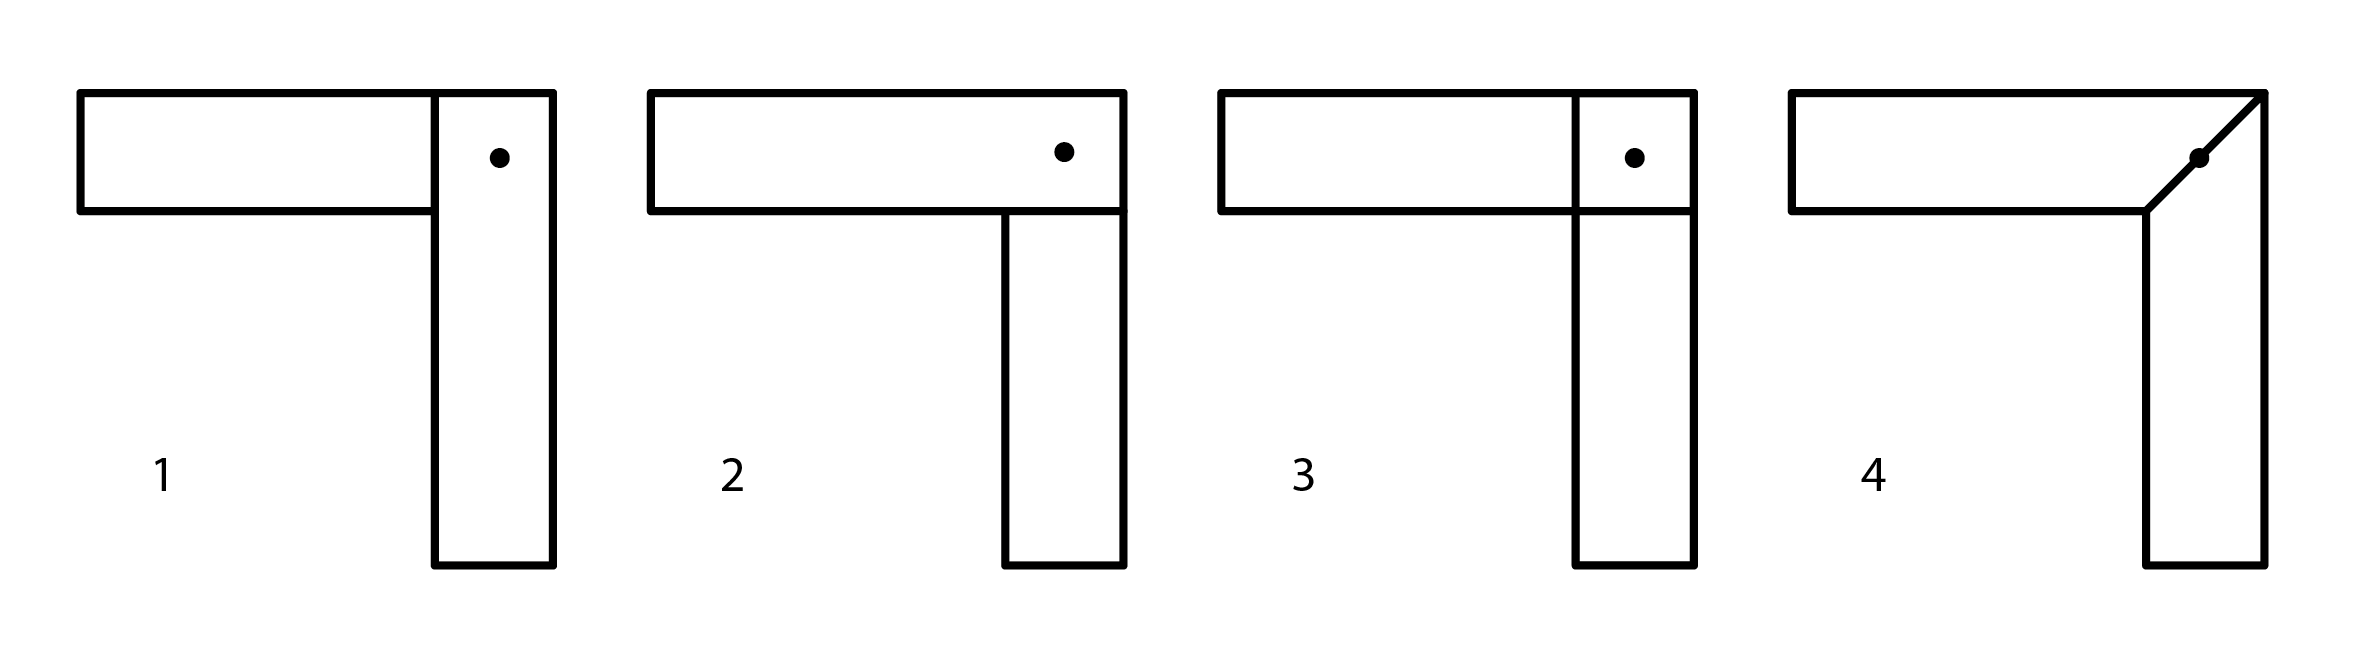
\includegraphics[width=0.8\columnwidth]{fig/ecken_variationen.png}
    \caption{Draufsicht auf Varianten der Modellierung einer Ecke.}
    \label{fig:concept:ecken_variationen}
\end{figure}

\begin{figure}[ht]
    \centering
    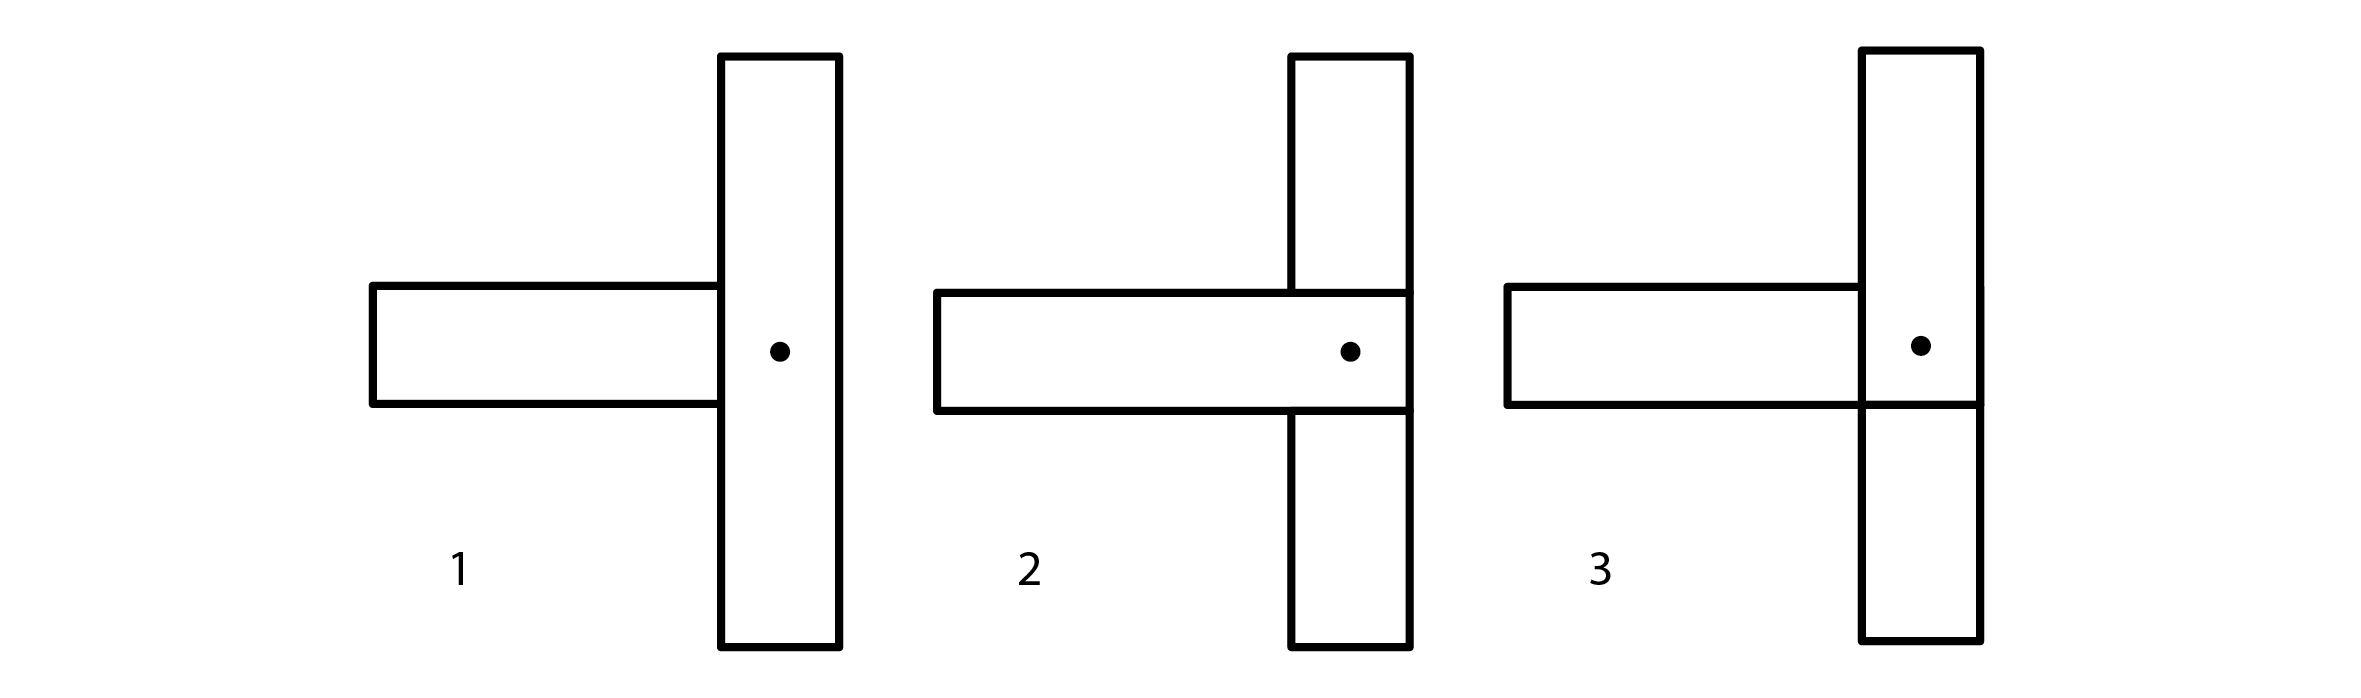
\includegraphics[width=0.8\columnwidth]{fig/t_joint_variationen.png}
    \caption{Draufsicht auf Varianten der Modellierung einer T-Kreuzung.}
    \label{fig:concept:t_joint_variationen}
\end{figure}

\begin{figure}[hb]
    \centering
    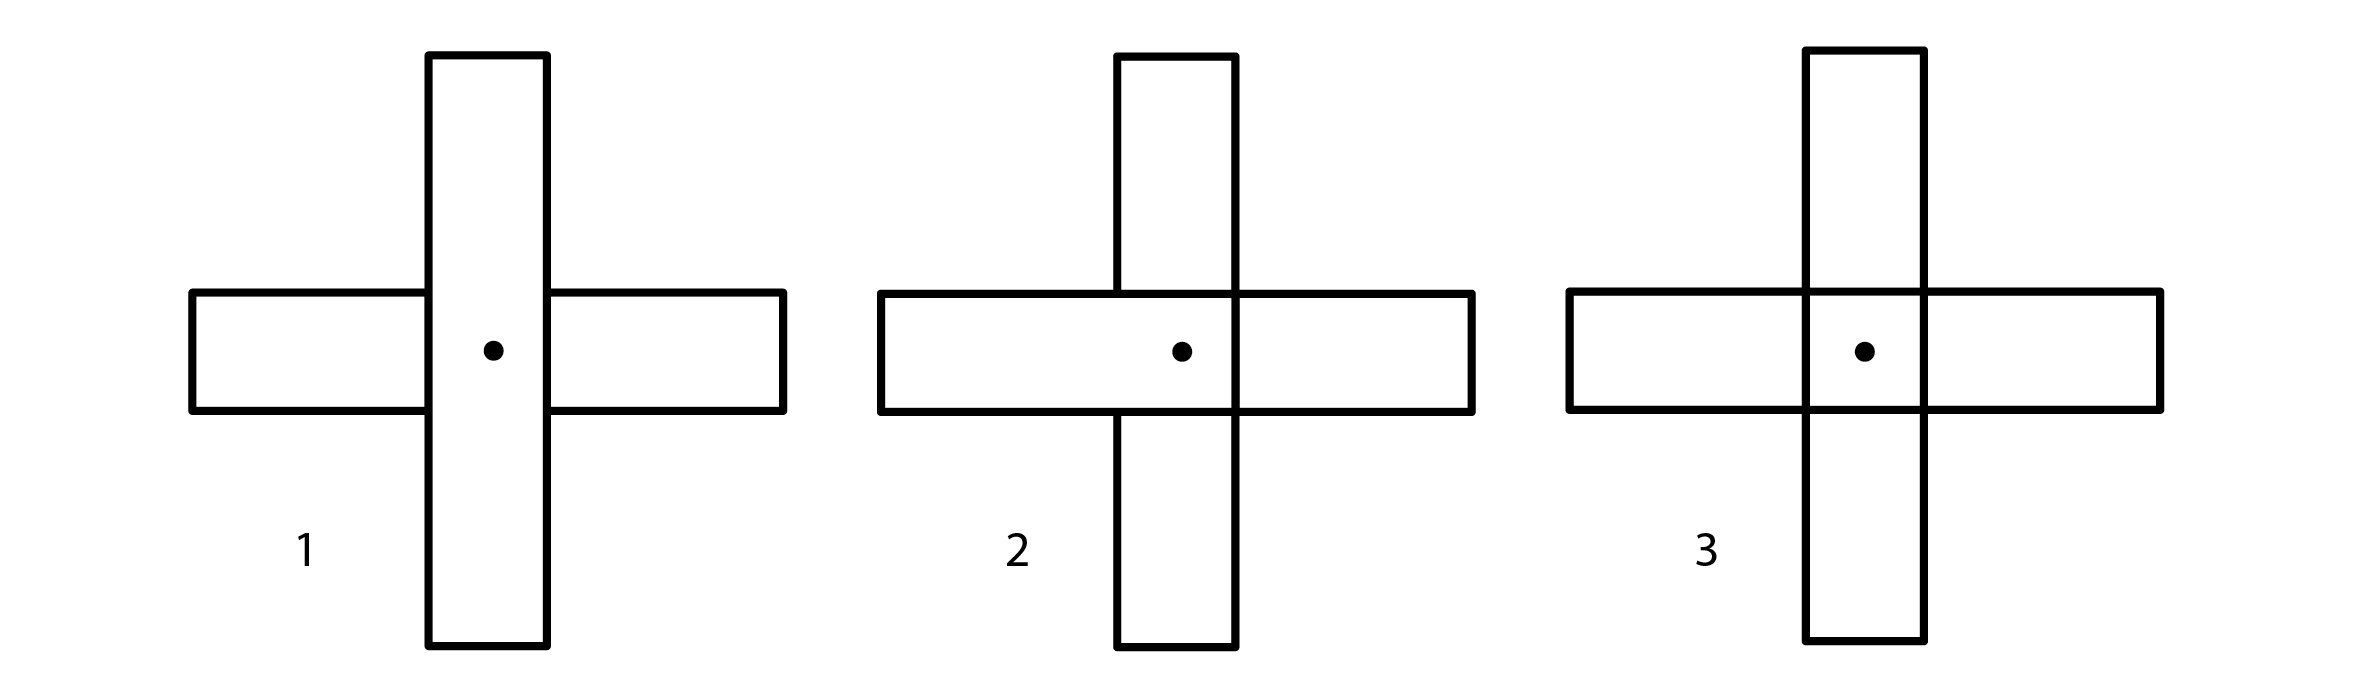
\includegraphics[width=0.8\columnwidth]{fig/x_joint_variationen.png}
    \caption{Draufsicht auf Varianten der Modellierung einer X-Kreuzung.}
    \label{fig:concept:x_joint_variationen}
\end{figure}

Sind diese Eigenschaften erfüllt, werden die Schnittpunkte der Richtungsvektoren entlang der lokalen X-Achsen beider Wandstücke errechnet.
Im Falle einer einfachen Ecke oder einer T-Kreuzung, existiert nur ein einzelnes Paar an Wandstücken, die sich im Mittelpunkt der Ecke oder der T-Kreuzung schneiden.
Der Unterschied ist lediglich die Stelle des Schnittpunkts relativ zu den beiden Wandstücken.
Sei \(w_1\) die Breite von einem und \(w_2\) die des anderen Wandstücks, so gilt nach Punkt~\ref{concept:tmp1} \(w_1 = w_2\).
Liegt der errechnete Schnittpunkt bei beiden Wandstücken näher als \(\frac{w_1}{2}\) entlang der lokalen X-Achse an einer der beiden Außenkanten handelt es sich um eine Ecke, da beide Wandstücke an diesem Punkt enden.
Falls der Schnittpunkt bei einem der beiden Wandstücke allerdings mindestens  \(\frac{w_1}{2}\) innerhalb des Wandstücks liegt, so handelt es sich um eine T-Kreuzung.
Ein Wandstück steht also auf einem Anderen.
Dies ist in den Abbildungen~\ref{fig:concept:ecken_variationen} und~\ref{fig:concept:t_joint_variationen} zu sehen. 
Werden für zwei unterschiedliche Paare die selben Schnittpunkte errechnet, so kann es sich entweder um eine mit drei Wandstücken modellierte T-Kreuzung oder X-Kreuzung handeln.
Treffen sich an dem Schnittpunkt zwei Ecken, ergibt sich daraus eine T-Kreuzung (siehe Fall 2 in Abbildung~\ref{fig:concept:t_joint_variationen}).
Teilen sich aber zwei T-Kreuzungen die selben Schnittpunkte, so sind alle Vorraussetzungen für eine eine X-Kreuzung gegeben (siehe Fall 1 in Abbildung~\ref{fig:concept:x_joint_variationen}).
Einen Sonderfall für Punkt~\ref{concept:tmp4} stellt eine X-Kreuzung dar - modelliert aus zwei sich schneidenden Wandstücken.
Dieser Fall ist in Abbildung~\ref{fig:concept:x_joint_variationen} mit der Variante Nummer 3 dargestellt.
Hier liegt der Schnittpunkt des Wandstück-Paares mindestens \(\frac{w_1}{2}\) innerhalb beider Wandstücke und keines der Wandstücke endet auf dem Anderen.
Durch das vorhergehende Kombinieren von Wandstücken werden die Fälle 3 aus Abbildung~\ref{fig:concept:t_joint_variationen} und 2 aus Abbildung~\ref{fig:concept:x_joint_variationen} eliminiert, denn dabei erfüllen jeweils zwei Wandstücke alle Eigenschaften, um nach Abschnitt~\ref{concept:combination_properties} zu einer Einheit verschmolzen zu werden.
So entsteht aus Fall 3 aus Abbildung~\ref{fig:concept:t_joint_variationen} der Fall Nummer 1 und auch Fall Nummer 2 aus Abbildung~\ref{fig:concept:x_joint_variationen} wird zu deren 1. Fall.

\subsection{Lösen von Beziehungen}\label{concept:solving_beziehungen}
Durch Ecken, T- und X-Kreuzungen werden ansonsten unabhängige Wandstücke miteinander verkettet.
Das kann zu Situationen führen, in welchen das einfache Anwenden eines Mauerwerksverbands Lücken in manchen Wandstücken hinterlässt.
Das Beispiel in Abbildung~\ref{fig:concept:loesen_von_beziehungen1} soll helfen diese Problematik zu veranschaulichen.
Zu sehen ist eine Konstellation von 4 Wandstücken, die in einer Kette durch 3 Ecken miteinander verbunden sind.
Das anzuwendende Modul hat die Dimensionen \([2, 1, 0.5]\). 
Die Höhe des Moduls ist für dieses Problem allerdings irrelevant, weshalb die folgenden Skizzen ausschließlich die Draufsicht auf die Situationen zeigen.
Wie in Kapitel~\ref{concept:mauerwerksverband} am Beispiel des Läuferverbands gezeigt, gibt es mehrere Möglichkeiten einem Eckplan zu folgen.
Solange die Reihenfolge weiterhin eingehalten wird, kann mit jeder Schicht des Eckplans begonnen werden einen Eckbereich aufzufüllen.
Das führt in dem Beispiel aufgrund des zwei-schichtigen Eckplans des Läuferverbands dazu, dass für jede der 3 Ecken zwei mögliche Startschichten existieren.
Dies resultiert demnach in insgesamt 8 unterschiedlichen Varianten, von welchen allerdings nicht alle zielführend sind.
In Abbildung~\ref{fig:concept:loesen_von_beziehungen2} ist eine Variante dargestellt, die Lücken in der Wand hinterlassen würde.
Das zunächst naheliegend wirkende Füllen der Löcher durch kleinere Bausteine ist nicht zulässig, da damit das Überbindemaß (siehe Kapitel~\ref{basics:Mauerwerksverband}) verletzt wäre.
Darum ist es notwendig eine Kombination an Startschichten über alle miteinander verbundenen Eckbereiche zu finden, die es ermöglicht die verbleibenden geraden Wandstücke im Anschluss durch einfaches Anwenden des Läuferverbands aufzufüllen, ohne dass Lücken entstehen.

\begin{figure}[]
    \centering
    \includegraphics[width=0.4\columnwidth]{fig/concept lösung von beziehungen1.png}
    \caption{Draufsicht auf eine Verkettung von 4 Wandstücken durch 3 dazwischenliegende Ecken.}
    \label{fig:concept:loesen_von_beziehungen1}
\end{figure}

\begin{figure}[]
    \centering
    \includegraphics[width=0.4\columnwidth]{fig/concept lösung von beziehungen2.png}
    \caption{Draufsicht auf eine unzulässige Lösung der Eckplankonfiguration.}
    \label{fig:concept:loesen_von_beziehungen2}
\end{figure}


\begin{figure}[ht!]
    \centering
    \begin{subfigure}[b]{0.4\columnwidth}
      \includegraphics[width=\columnwidth]{fig/concept lösung von beziehungen3.png}
      \caption{Eine zulässige Lösung.}
      \label{fig:concept:loesen_von_beziehungen3}
    \end{subfigure}
    \hfil
    \begin{subfigure}[b]{0.4\columnwidth}
      \includegraphics[width=\columnwidth]{fig/concept lösung von beziehungen4.png}
      \caption{Die darüberliegende Schicht.}
      \label{fig:concept:loesen_von_beziehungen4}
    \end{subfigure}
  \caption{Eine mögliche Lösung und die durch die Eckpläne entstehende zweite Lösung für die darüber liegende Schicht.}
  \label{fig:concept:loesen_von_beziehungen3und4}
\end{figure}

Ein Verfahren, welches für das vorliegende Beispiel des halbversetzten Läuferverbands, dessen sehr einfachen Eckplans und dem durch seine praktische Form gewählten Moduls Lösungen findet, löst nicht zwangsläufig auch eine beliebig andere Situation.
Ebenfalls führt das Miteinbeziehen der 3. Dimension, also der Höhe der beteiligten Wandstücke, zu einer erheblichen Vervielfachung möglicher Eck-Konstellationen.
Zieht man etwa das Beispiel aus Abbildung~\ref{fig:concept:combination_example_base} heran und erweitert es durch Einfügen weiterer Wandstücke um Ecken an den Außenkanten von Bereich 1, 3, 4, 5+6 und 7, an welchen beliebig weitere verkettete Wandstücke in sich geschlossene Kreise bilden, so können sogar nicht lösbare Fälle auftreten.
Durch die Anzahl der Schichten des Eckplans eines Mauerwerksverbands und die Anzahl der miteinander verketteten Wandstücke baut sich schnell ein großer Lösungsraum auf.
Aufgrund der Einschränkung eine mögliche Lösung lediglich mit zulässig oder unzulässig bewerten zu können, sind herkömmliche Optimierungsverfahren nicht in der Lage das Problem zu lösen.
Diese benötigen meistens eine sogenannte \textit{Fitness Funktion}, welche die Güte der derzeitigen Lösung angibt und dem Optimierungsverfahren sozusagen eine Richtung weist, in der ein lokales Minimum oder Maximum dieser Funktion zu erwarten ist.
Wählt man die \textit{Fitness Funktion} sinnvoll, kann damit ein kontinuierlicher Lösungsraum effizient nach einer passablen Lösung durchsucht werden.
In dem vorliegenden Fall gibt es allerdings, wenn überhaupt, nur einige wenige zulässige Lösungen, die an den Startindizes der Pläne der jeweilgen Eckbereiche gekoppelt sind.
Diese Startindizes weisen aber nicht dieselben Eigenschaften auf, wie kontinuierliche Parameter, die durch kleine Veränderungen eine etwas bessere oder schlechtere Lösung erzeugen.
Das Ändern eines Startindex einer einzelnen Ecke kann zwar eine Lösung mit einer reduzierten Anzahl an Lücken liefern, gibt aber deswegen keine Richtung vor in der man noch bessere Lösungen erwarten kann.
Außerdem ist auch eine Lösung mit einer einzigen Lücke nicht zulässig, da dies die Stabilität eines Wandstücks stark beeinflussen könnte.

Darum bleibt zunächst nur die Brute-Force-Methode (auch als Exhautionsmethode bekannt), also das Berechnen sämtlicher Konfigurationen bis eine zulässige gefunden wurde.
Allerdings fällt schnell auf, das das Wählen eines einzigen Startindex für eine Ecke, alle direkt und indirekt damit verketteten anderen Ecken beinflusst.
Wählt man in dem obigen Beispiel in Abbildung~\ref{fig:concept:loesen_von_beziehungen3} etwa die untere Ecke aus und legt deren Startindex auf die abgebildete Situation fest, so verbleibt ohnehin nur noch eine zulässige Konfiguration für die darüber liegende Ecke.
Andernfalls befände man sich in der Situation aus Abbildung~\ref{fig:concept:loesen_von_beziehungen2}, welche keine zulässige Lösung darstellt.
Setzt man nun den Eckplanindex für diese Ecke ebenfalls fest, zwingt man deren zweiten Nachbarn zwangsläufig in die abgebildete Situation, da der zweite Fall wieder zu einer unzulässigen Lösung führen würde.
Da sich an einem Wandstück übereinander mehrere Ecken befinden können, bildet sich damit ein Abhängigkeitsgraph zwischen allen miteinander verketteten Wandstücken.
Dieser kann wie folgt erstellt werden:

\begin{enumerate}
    \item Wähle eine Startecke und finde alle darüber- und darunterliegenden Ecken, die durch Festlegen eines Index einer Ecke in einer dieser Schichten direkt davon betroffen sind. Dies stellt den ersten Knoten des Abhängigkeitsgraphen dar.
    \item Finde alle Nachbarn aller zuvor gefunden Ecken.
    \item Wiederhole für jeden Nachbarn das Vorgehen aus dem ersten Schritt. Daraus resultieren die nächsten Knoten, welche mit dem Vorgängerknoten verbunden werden.
    \item Stößt man dabei auf einen schon existierenden Knoten, so bricht man diesen Pfad an der Stelle ab. Dieser Fall tritt zum Beispiel auf, wenn in dem Modell ein abgeschlossener Raum exisitiert.
\end{enumerate}

Nun kann das Modell mithilfe des Graphen einfach ähnlich einer Breitensuche durchlaufen und ausgehend von den Startindex des Eckplans eines Knotens die Indizes von dessen Nachbarn in passender Weise gewählt werden.
Dies wiederholt man für alle Nachbarn des derzeitigen Knotens, im nächsten Schritt für deren Nachbarn, solange bis alle Knoten einen Startindex zugewiesen bekommen haben.
In ungünstigen Situationen hängt das Finden einer passenden Lösung von dem Startknoten ab.
Dies tritt manchmal auf, wenn mehrere Kreise im Abhängigkeitsgraph exisitieren.
Wird für den gewählten Startknoten mithilfe des Verfahrens keine zulässige Lösung gefunden, so muss ein anderer Startknoten ausprobiert werden.
Findet man für keinen Startknoten eine valide Lösung, so exisitiert für das Modell und den Modulen der gewünschten Mauerwerksverbände keine naheliegende, lückenlose Bausteinkonfiguration.

\subsection{Öffnungen}
Neben Wänden sind Öffnungen ein integraler Bestandteil bei der Planung von Gebäuden.
Öffnungen sind Bereiche an welchen das Mauerwerk unterbrochen wird, um Lücken zu schaffen, in die später zum Beispiel Fenster oder Türen eingesetzt werden können.
Da eine Öffnung nicht ohne eine Wand existieren kann, liegt es nahe die dazugehörigen Informationen in der Wand zu hinterlegen, die von der Öffnung betroffen ist.
Eine Öffnung kann ebenfalls als quaderförmiger Körper angesehen werden, der einen Bereich innerhalb eines Wandstücks definiert, an dem später keine Bausteine gelegt werden dürfen.
In dieser Arbeit besitzt dieser Quader die selbe Orientierung wie das dazugehörige Wandstück und schneidet zunächst immer durch die gesamte Breite der Wand.
Daher sind nur Position, Länge und Höhe des Quaders von Bedeutung für das Wall Detailing.
Da es allerdings üblich ist einen sogenannten Sturz über der eigentlichen Öffnung eines Fenster oder einer Tür anzubringen, muss auch für dieses Objekt Platz im Wandstück geschaffen werden. 
Der Sturz ist etwas länger als die Länge der Öffnung und liegt an beiden Seiten auf dem Mauerwerk auf, um den Bausteinen darüber eine stabile Grundlage zu bieten.
So bleibt die Stabilität der Wand trotz Öffnungen erhalten.

\subsection{Wandenden}
Stehen eine oder beide Kanten eines Wandstücks allein, ohne dort über eine Beziehung mit einem anderen verbunden zu sein, muss der Mauerwerksverband zu einem geraden Abschluss gebracht werden.
Häufig ist dies nur möglich, indem man für manche Bausteine die Länge des verwendeten Moduls anpasst.

\begin{figure}[htb]
    \begin{subfigure}[b]{0.5\columnwidth}
      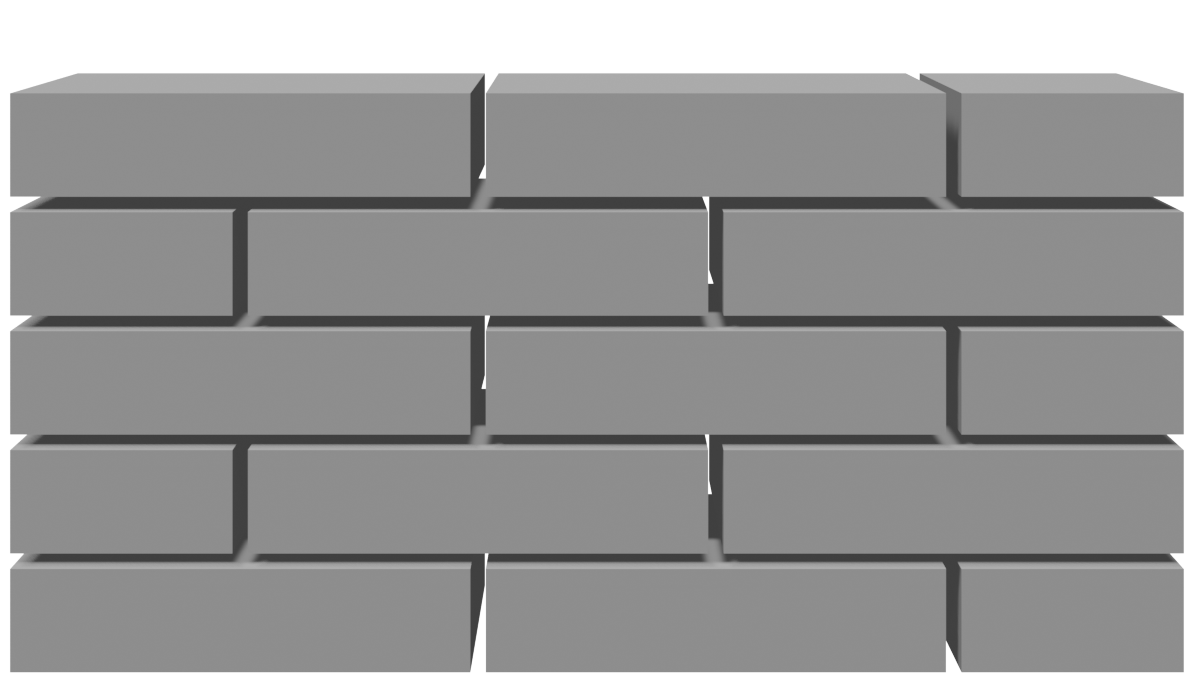
\includegraphics[width=\columnwidth]{fig/concept_wall_endings_1.png}
      \caption{Läuferverband.}
      \label{fig:concept:lauferverband_ending}
    \end{subfigure}
    \hfill
    \begin{subfigure}[b]{0.5\columnwidth}
      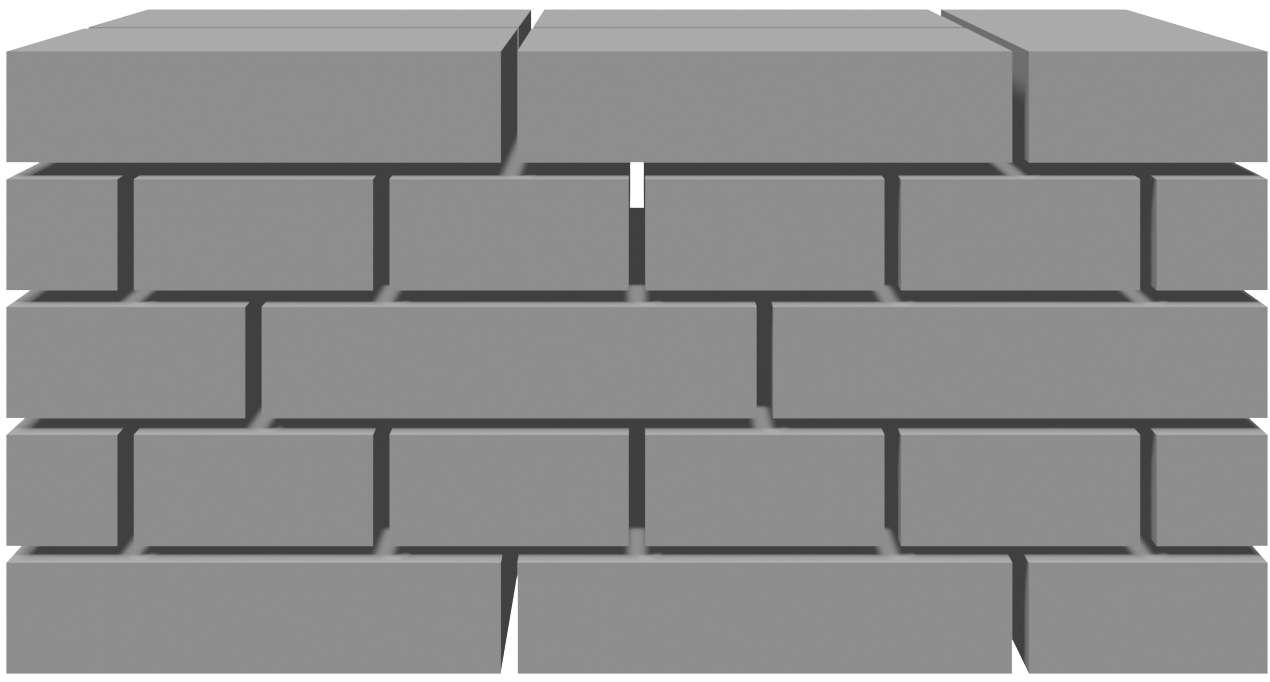
\includegraphics[width=\columnwidth]{fig/concept_wall_endings_2.png}
      \caption{Kreuzverband.}
      \label{fig:concept:kreuzverband_ending}
    \end{subfigure}
  \caption{Wandenden verschiedener Mauerwerksverbände.}
\end{figure}

In Abbildung~\ref{fig:concept:lauferverband_ending} werden für den Läuferverband Bausteine mit halber Modullänge und für den Kreuzverband in der Abbildung daneben zwei angepasste Versionen des Moduls benötigt:
Erneut ein Bausteinformat mit halber Modullänge um die Läuferverbandschichten des Kreuzverbands abzuschließen und ein Bausteinformat, dessen Länge sich aus der halben Modulbreite bildet und für den Abschluss der Kopfverbandschichten notwendig ist.
Aber nicht nur an Wandenden muss ein Mauerwerksverband mit einer geraden Kante abgeschlossen werden.
Auch an den zuvor angesprochen Öffnungen ist dies für die Schichten erforderlich, die durch die Öffnung geteilt werden.
Für den Fall, dass das vollständige Detailing eines Modells das Anpassen des gewünschten Moduls notwendig macht, muss diese Information neben den errechneten Transformationen der Bausteine ebenfalls in das Ergebnis integriert werden.
Somit erhält jeder Baustein aus diesem Grund zusätzlich eine Beschreibung über dessen Dimensionen.

\section{Wall Detailing}
\label{concept:wall_detailing}
Als \glqq{}Wall Detailing\grqq{} (sprich das \glqq{}Detailieren von Wänden\grqq{}) wird in dieser Arbeit der Vorgang bezeichnet ein als geometrischer Körper definiertes Wandstück in konkretes Mauerwerk zu überführen.
Dieser Vorgang wendet die zuvor behandelten Konzepte an, um Lösungen für beliebig komplexe Gebäudemodelle zu errechnen.
Als Lösung sollen nur diejenigen Bausteinmengen gelten, die sämtliche von Wandstücken abgedeckten Bereiche lückenlos mit Bausteinen füllen, während gleichzeitig die gewünschten Mauerwerksverbände eingehalten werden.
Das nachfolgende schrittweise Verfahren weist aufgrund der ähnlichen Zielsetzung zwangsläufig Ähnlichkeiten zu dem von Usmanov et al. auf, das bereits in Kapitel~\ref{related:digital_plan_of_brickwork_layout} zusammengefasst wurde.

\begin{enumerate}
    \item Extrahieren relevanter Informationen wie Geometrie und Typ-Annotationen aus dem vorgegebenen Gebäudemodell. Dabei interessieren in erster Linie Wände und deren Öffnungen sowie gewünschte Module und Mauerwerksverbände (siehe Abschnitt~\ref{concept:mauerwerksverband}).
    \item Anwenden des vorgegebenen Moduls für jedes gefundene Wandstück. Das führt zu einer schichtweisen Repräsentation jedes Wandstücks. Dies erleichtert es später Operationen an und zwischen mehreren Wandstücken durchzuführen.
    \item Finden und Kombinieren von Wandstückverbänden nach Abschnitt~\ref{concept:combination_properties}.
    \item\label{concept:wall_detailing_tmp1} Finden und Lösen von anderen Beziehungen wie Ecken T- und X-Kreuzungen nach Abschnitt~\ref{concept:corner_etc_properties} (Finden) und Abschnitt~\ref{concept:solving_beziehungen} (Lösen).
    \item Schichtweises Anwenden der Öffnungen jedes Wandstücks. Dabei werden alle betroffenen Schichten in passender Weise geteilt und deren Länge reduziert.
    \item Schichtweises Anwenden der den Wandstücken zugewiesenen Mauerwerksverbände. Dazu gehören sowohl die besonderen Bereiche aus Punkt~\ref{concept:wall_detailing_tmp1}, als auch gerade Wandabschnitte und allein stehende Wandenden.
    \item\label{concept:wall_detailing_tmp2} Finden von (direkten) Nachbarschaftsbeziehungen zwischen Bausteinen.
    \item Konvertieren in das für die nachfolgende Bauplandeduktion notwendige Format.
\end{enumerate}

Das Ergebnis dieser Schritte ist eine Menge aus Bausteinen, nachfolgend auch als \textit{Konstruktionsplan} bezeichnet.
Durch die Berechnungen in Schritt~\ref{concept:wall_detailing_tmp2} werden bereits die grundlegensten Beziehungen zwischen den Bausteinen hergestellt.
Eine Aussage darüber in welcher Reihenfolge die Bausteine gesetzt werden müssen, um das geplante Gebäude unter Berücksichtigung etwaiger physikalischer oder anderer Einschränkungen zu errichten, wird allerdings noch nicht getroffen.
Dazu müssen Schritt für Schritt Teilmengen aus der Gesamtmenge an Bausteinen extrahiert werden, die nur diejenigen Bausteine beinhalten, die in einer bestimmten Situation gelegt werden können.
Welche das sind, soll anhand vorgebener Regeln ausgewertet werden können.
Diese Regeln können dafür verwedet werden bestimmte Voraussetzungen an einen Baustein zu setzen, um zum Beispiel das Ablegen eines Bausteins zu verhindern, unter dem sich weder fester Boden, noch ausreichend andere Bausteine befinden.
Denn setzt man einen Baustein mitten in der Luft ab, so fällt er in der echten Welt aufgrund der auf ihn einwirkenden Gravitation zu Boden.
Außerdem weisen unterschiedliche Bausteinarten und Umgebungen, in die man das Gebäude mithilfe des zuvor errechneten Konstruktionsplans errichten möchte, womöglich unterschiedliche Einschränkungen auf.
So ist es notwendig je nach Situation voneinander abweichende Regelsets auf dem Konstruktionsplan anzuwenden zu können.
Die Möglichkeit der nachträglichen Definition dieser Regeln verhindert zusätzlich die Notwendigkeit den Konstruktionsplan für sich unterscheidene Situationen neu berechnen zu müssen.

\section{Regelbasierte Bauplandeduktion}
Ontologien bieten verschiedene Werkzeuge an, mithilfe derer auf streng definierten Objekttypen und deren Relationen zueinander konkrete Instanzen gruppiert und gefiltert werden können.

\begin{enumerate}
  \item Klassendefinition aufstellen
  \item Relationen definieren
  \item Bild Einfügen
  \item Regel einführen (und versuchen diese nachträglich mit owlready reinzuhauen)
  \item Reasoner ausprobieren und schrittweise bausteine als gesetzt markieren um neue Menge an möglichen steinen rauszubekommen
\end{enumerate}
\chapter{Realisierung}
\section{Modellierung}
Blenderplugin, IFCWallTypes Module die das Raster vorgeben etc.

\section{Wall Detailing}
Als \glqq{}Wall Detailing\grqq{} (sprich das \glqq{}Detailieren von Wänden\grqq{}) wird in dieser Arbeit der Vorgang ein als geometrischer Körper definiertes Wandstück in ein konkretes Mauerwerk zu überführen, bezeichnet.
Innerhalb des IFC Standards werden einige mathematische/geometrische Repräsentationen der sogennanten \textit{IFCWall} unterstützt, um neben einfachen Boxen auch komplexere Formen abbilden zu können.
Beispielsweise ist es möglich in das Modell eines Hauses zunehmend dünner werdende Wandstücke, kurvige Wandstücke oder Wandstücke, welche nur durch ein arbiträres Vieleck beschrieben werden können zu integrieren.
Allerdings ist es für die Fallstudien dieser Arbeit zunächst ausreichend nur Wandstücke, welche als einfacher geometrischer Quader vorliegen, zu beachten.
Das nachfolgende schrittweise Vorgehen weist aufgrund des annähernd gleichen Ergebnisses zwangsläufig Ähnlichkeiten zu dem von Usmanov et al. auf \cite{Usmanov2021}.

\subsection{Konvertieren des IFC zu BREP}
Den ersten Schritt stellt das Extrahieren aller notwendigen Daten aus dem vorliegenden IFC Modell dar.
Für die Fallstudien dieser Arbeit sind sowohl alle Objekte des Typs \textit{IFCWall} als auch die, etwa durch Fenster oder Türen entstehenden, daran angeknüpften Objekte vom Typ \textit{IfcOpeningElement} (siehe \ref{basics:IfcOpeningElement}) von Interesse.
Zusätzlich werden aus den, in den \textit{IfcPropertySets} der Wandstücke hinterlegten Daten, Informationen über das zu verwendende Modul ausgelesen.
Mithilfe der Werkzeuge der in Kapitel \ref{basics} vorgstellten Python Bibliothek \textit{ifcopenshell} (siehe \ref{basics:ifcopenshell}) ist dies intuitiv möglich.
TODO Sätze zum Code, Code TODO kleines Klassendiagram von Wall/WallLayerGroup und Opening und BrickInformation

\subsection{Überprüfen der modellierten Wände}
\subsubsection{Filtern}
Da sich diese Arbeit vorerst ausschließlich mit quaderförmigen Wandstücken beschäftigt, müssen zunächst alle zuvor extrahierten Wandstücke auf diese Eigenschaft geprüft werden.
Somit ist gewährleistet, dass lediglich passende Wandstücke an die nachfolgenden Schritte weitergegeben werden.
TODO Satz zum Code, Code iscubic

\subsubsection{Anwenden des Moduls}
Mit dem zu jedem Wandstück festgelegten Modul werden nun alle Wandstücke in Schichten aufgeteilt.
Deren Höhe entspricht im Normalfall der Höhe des jeweilgen Moduls.
Dies erleichtert es im Anschluss Berechnungen an Wandstücken durchzuführen und Beziehungen zwischen ihnen zu finden.
Lediglich die oberste Schicht kann durch falsch modellierte Wandstücke eine niedrigere Schichthöhe aufweisen.
Dies ist der Fall, wenn die Gesamthöhe des Wandstücks nicht exakt einem Vielfachen der Höhe des Moduls entspricht und ein nicht aufzuteilender Rest existiert.

\subsubsection{Kombinieren passender Wandstücke}
Eine solche Beziehung stellen etwa Wandstücke dar, die zwar in dem Modellierungsprozess des Gebäudes durch mehrere einzelne Objekte realisiert wurden, eigentlich aber eine Einheit darstellen.
Daher werden in diesem Schritt alle Wandstücke miteinander verglichen und eventuell kombiniert, sodass jeweils ein gefundes Paar durch ein einzelnes Wandstück representiert wird.
Um zwei Wandstücke zu kombinieren müssen folgende Eigenschaften gelten:
* Beide Wandstücke verwenden das selbe Modul und sind während der Modellierung mit den gleichen Wandtyp annotiert worden. -> Dies verhindert das Kombinieren unterschiedlich dicker Wände
* Die lokalen Z-Achsen beider Wandstücke sind parallel. -> Dies verhindert das Kombinieren ungleich rotierter Wandstücke
* Sie stehen auf der selben Höhe oder versetz um ein Vielfaches der gemeinsamen Modulhöhe.
* Mindestens eine Schicht des einen Wandstücks berührt oder überlappt eine des anderen.

TODO: Bilder und Erklärung der verschiedenen Fälle
Steht ein Wandstück in X-Richtung versetzt auf einem anderem, so ist es notwendig diesen Versatz während dem nachfolgenden Detailing zu berücksichtigen.
Ignoriert man diesen Versatz kann dies zu den in Abbildung TODO gezeigten Fehlern führen.
Dieser, nachfolgend als \textit{x\_offset} bezeichnete Versatz ist definiert durch die Differenz zwischen der kleinsten lokalen X-Koordinate aller Schichten eines Wandstückes und der lokalen X-Koordinate der zu betrachtenden Schicht.
Der daraus resultierende Wert wird später dazu verwendet den anzuwendenden Mauerwerksverband an erst an der passenden Stelle zu beginnen.
Dadurch erzielt man einen einheitlichen Verband über das gesamte Wandstück und verhindert den in Abbildung TODO Fehlerfall.
Eine weitere Eigenschaft, die aus dem Kombinieren zweier Wandstücke entstehen kann, ist das vorhandensein unterbrochender Schichten beziehungsweise mehrerer Schichten auf einer Höhe innerhalb eines Wandstückes.
Dies ist ebenfalls in Abbildung TODO dargestellt.
Durch das Einbeziehen des \textit{x\_offset} können derartige Situationen jedoch ebenfalls gelöst werden, da für jedes Teilstück einer Schicht ein eigener \textit{x\_offset} berechnet wird.
Auch dies ist der Abbildung TODO zu entnehmen.

\subsubsection{Beziehungen finden}
Durchlaufe alle Wandstücke und schau, ob diese andere berühren.
Dadurch können Ecken, T-Kreuzungen und Kreuzungen gefunden werden.
Schwierigkeiten: Verschiedenste Arten solche Ecken und Kreuzungen zu modellieren 

\subsection{Lösen der Beziehungen}
Je nach gewählten Verband müssen z.B. Ecken (deren Baupläne im vornherein definiert wurden) so angeordnet werden, dass die dazwischenliegenden Wandstücke lückenlos eingefüllt werden können.
Dafür muss ein sogenannter "plan\_offset" für jede Wand und jede Ecke gefunden werden. Dieser gibt an, an welchem Index der Bauplandefinition das Wandstück (von unten) beginnen muss, um insgesamt einen einheitlichen Wandkörper ohne Lücken zu bilden.
Voraussetzung dafür ist natürlich ein passender Eckplan zu dem gewählten Verband. 

Schwierigkeiten: Eckpläne insgesamt, Ecken ragen in die sie bildenden Wände hinein. Diese müssen dementsprechend verkleinert werden.

\subsection{Anwenden der Lösung}
Ablaufen aller Ecken und Wände und einsetzen der Ziegel gemäß den gefundenen Lösungen.

\subsection{Export}
Abhängigkeitsgraph und Ontologie für Regelwerk
\chapter{Proof of Concept}
Nun wird das realisierte Konzept anhand der in Kapitel~\ref{scenarios} vorgestellten Fallstudien auf Applikabilität geprüft.
Aus den Ergebnissen dieses Kapitels kann im Anschluss ein Fazit gezogen und ein potentieller Ausblick auf künftige Erweiterungen des Konzepts gegeben werden.

\section{Von 3D Gebäudeplan zu Bauplanentwurf}
Zunächst müssen für Szenario 1 und 2 Gebäudepläne in einem Konstruktionsplaner modelliert werden.
Dazu wurde, wie schon in Kapitel~\ref{real:modellierung} beschrieben, die 3D Modellierungs-Software Blender herangezogen (siehe Kapitel~\ref{basics:blender}).
Diese kann mit der frei verfügbaren Erweiterung \textit{blenderbim} zu einem funktionsfähigen BIM Editor mit \textit{IFC} Unterstützung ausgebaut werden (auch diese Technologien wurden bereits in den Kapiteln~\ref{basics:blenderbim} und~\ref{basics:ifc} vorgestellt).
Darin lassen sich sowohl individuelle Wandtypen erstellen, als auch mithilfe der \textit{IfcProperties} Annotationen über Modul und Rastermaße daran anhängen.
Mit den in Kapitel~\ref{concept:raster} definierten Modellierungseinschränkungen, deren Umsetzung in Kapitel~\ref{real:modellierung} thematisiert wurde, konnte die Modellierungsphase sowohl erleichtert, als auch beschleunigt werden.

\subsection{Szenario 1}\label{poc:scenario1}
Die Modellierung der zwei sich in der Wanddicke unterscheidenden Versionen des 20 Meter hohen Turms mit einer Grundfläche von 10$\times$10 Metern in Blender war wenig komplex.
Es bedarf lediglich vier Wände, die einen quadratischen Raum bilden.
Das vollständige Gebäudemodell ist in Abbildung~\ref{fig:poc:scenario1 modell} zu sehen.
\begin{figure}[ht!]
  \centering
  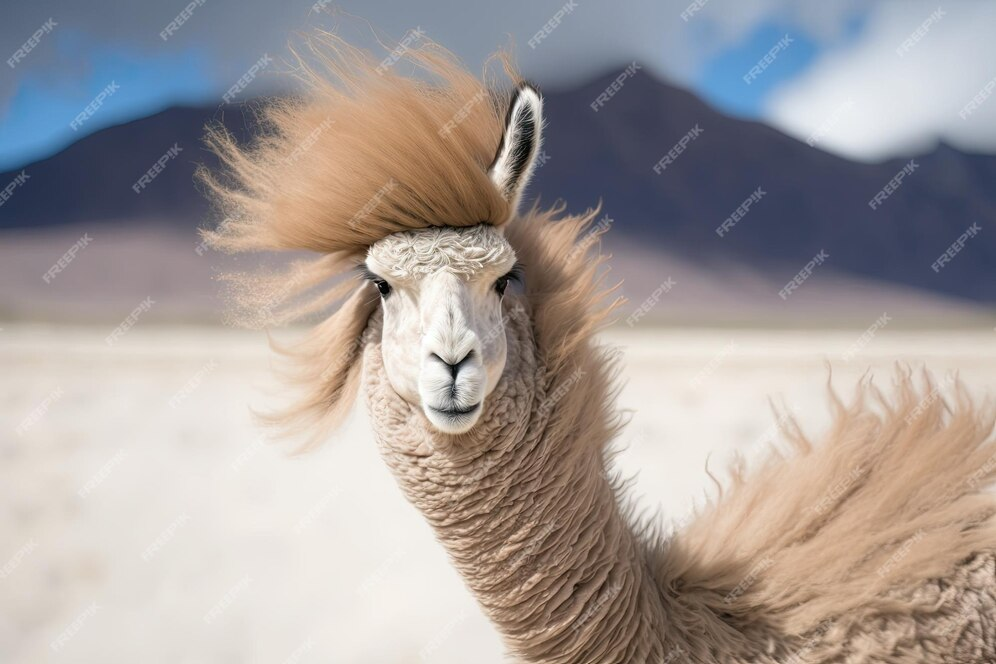
\includegraphics[width=0.6\columnwidth]{fig/TODO.jpg}
  \caption{TODO IFC Modell der beiden Türme.}\label{fig:poc:scenario1 modell}
\end{figure}
Das Ergebnis nach Anwenden der drei verschiedenen Mauerwerksverbände ist wie erwartet.
Die verschiedenen Verbände lassen sich wie in Kapitel~\ref{real:verband} gezeigt in den Programmcode einpflegen.
Das Basismodul ist überall dort zu sehen, wo ein gerader Wandabschnitt vorliegt.
Alle vier Eckbereiche sind korrekt identifiziert worden, denn dort wurde der für den jeweiligen Mauerwerksverband definierte Eckplan passend umgesetzt.
Im Falle des Kreuz- und Kopfverbandes wurde das Basismodul dabei etwas verkürzt.
Die drei den Bauplanentwürfe werden als Json-Dateien ausgegeben.
Darin sind alle in Abschnitt~\ref{real:export} angegebenen Informationen enthalten.
In Abbildung~\ref{fig:poc:result_scenario1} sind die Meshes der drei mit Bausteinen realisierten Türme zu sehen.

\begin{comment}
\begin{figure}[htb]
    \begin{subfigure}[b]{0.5\columnwidth}
      \includegraphics[width=\columnwidth]{fig/render_läuferverband50.png}
      \caption{Bla.}\label{fig:poc:render_laeuferverband50}
    \end{subfigure}
    \hfill
    \begin{subfigure}[b]{0.5\columnwidth}
      \includegraphics[width=\columnwidth]{fig/render_crossbond.png}
      \caption{Bla.}\label{fig:poc:render_crossbond}
    \end{subfigure}
    \begin{subfigure}[b]{1.0\columnwidth}
      \includegraphics[width=\columnwidth]{fig/render_headbond.png}
      \caption{Bla.}\label{fig:poc:render_headbond}
    \end{subfigure}
    \caption{Ergebnisse.}\label{fig:poc:result_scenario1}
  \end{figure}
\end{comment}

\subsection{Szenario 2}\label{poc:scenario2}
Die Modellierung dieses Szenarios war aufgrund der Fenster und Türen ein wenig anspruchsvoller.
Das dafür vorgesehene Vorgehen innerhalb der BIM Erweiterung für Blender ist zunächst etwas versteckt.
Zumindest ist das Hinzufügen neuer Tür- und Fensterarten ist der Definition neuer Wandarten sehr ähnlich.
Das finale Modell ist in Abbildung~\ref{fig:poc:scenario2 modell} zu sehen.
In Kapiteln~\ref{concept:openings} und~\ref{real:openings} wurde bereits aufgeführt, wie Öffnungen aus dem Modell extrahiert und als Teil des Wall-Detailings berücksichtigt werden.
Das in Abbildung~\ref{fig:poc:scenario2 ergebnis} zu sehende Ergebnis zeigt die korrekte Umsetzung der Fenster und Türbereiche.
TODO Übergange zwischen Wänden verschiedener Dicken.
TODO T-Kreuzungen?

\begin{figure}[hb]
  \centering
  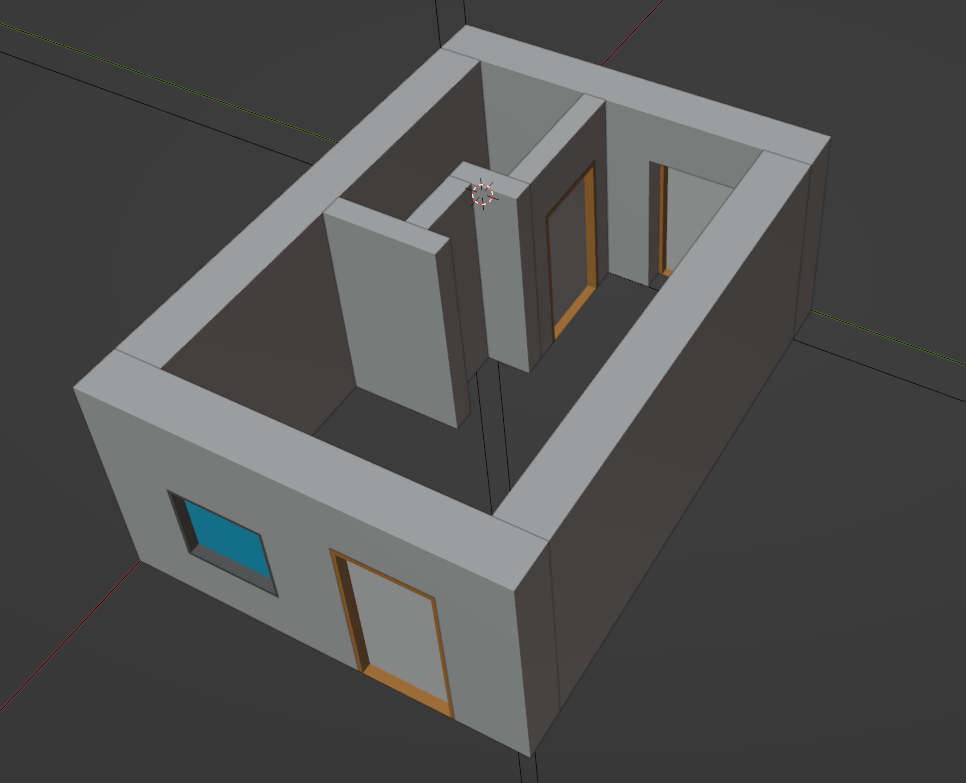
\includegraphics[width=0.5\columnwidth]{fig/scenario1_screenshot.png}
  \caption{TODO 3D Modell.}\label{fig:poc:scenario2 modell}
\end{figure}

\begin{figure}[ht!]
  \centering
  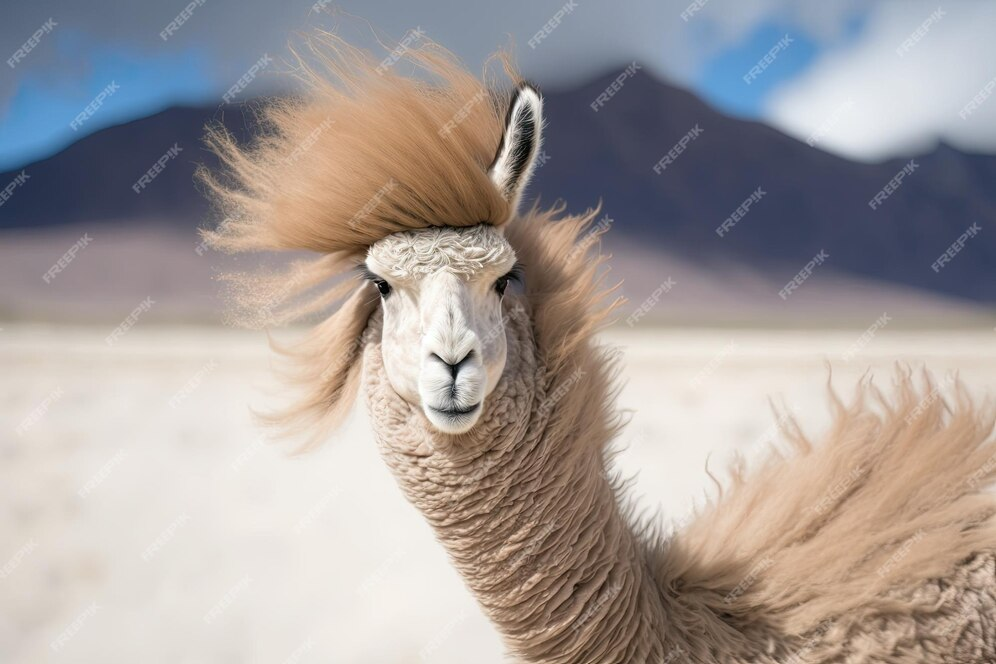
\includegraphics[width=0.6\columnwidth]{fig/TODO.jpg}
  \caption{TODO Ergebnis Szenario 2.}\label{fig:poc:scenario2 ergebnis}
\end{figure}

\subsection{Szenario 3}\label{poc:scenario3}
\section{Regelbasierte Bauplandeduktion aus einem Bauplanentwurf}
\chapter{Fazit und Ausblick}
Mit dem Ergebnis dieser Arbeit konnten erstaunlich viele Teilprobleme bei der Überführung eines 3D Modells eines Gebäudes in konkretes Mauerwerk identifiziert und für viele davon Lösungen gefunden werden.
Vor allem durch die Unterstützung beliebiger Basismodule und das einfache Definieren neuer Mauerwerksverbände unterscheidet sich das erarbeitete Konzept von einigen in Kapitel~\ref{related} vorgestellten Veröffentlichungen.
Mit der flexiblen Definition von Regelsets innerhalb einer Ontologie konnte der Grundstein für eine komplexe regelbasierte Analyse des errechneten Bauplanentwurfs gelegt werden.
Dies konnte anhand diverser Fallstudien und Szenarien belegt werden.
Dennoch gibt es selbstverständlich einige Erweiterungsmöglichkeiten.
Insbesondere das programmatische Lösen kritischer Bereiche wie etwa T-Kreuzungen und anderen Situationen, die nicht zuvor in den beteiligten Mauerwerksverbänden eingepflegt wurden, stellt ein interessantes aber komplexes Problem dar.
Hier bietet sich das Verwenden von Optimierungsansätzen aus der Domäne des \textit{Bin Packings} oder das darauf gezielte Trainieren von \textit{Machine Learning Algorithmen} an.
Damit könnten eventuell auch Probleme wie abgerundete Ecken und Ecken, die keinen 90\textdegree{} Winkel aufweisen umgesetzt werden.
Aber auch der Anwendungsfall nicht quadratischer Wandstücke kann mit dem vorliegenden Grundgerüst der schichtweisen Betrachtung eines Wandabschnitts durch \glqq{}Ausstanzen\grqq{} eines Vielecks daraus berücksichtigt werden.
Eine Erweiterung um eine simulative Komponente ist ebenfalls denkbar.
Darin könnten etwa Statik-Berechnungen durchgeführt werden, um potenziell fehlerhafte Bereiche im Gebäudemodell ausfindig zu machen.

Fugengröße in Brickinformation integrieren
TODO Rasterlose modelle und Wanddimensionen untersützen, die keinem Raster entsprechen -> das ermöglicht das fremder modelle
\listoffigures
\printbibliography{}
\end{document}
